\documentclass[11pt,a4paper]{article}
\usepackage[utf8]{inputenc}
\usepackage[T1]{fontenc}
\usepackage[french]{babel}
\usepackage{lmodern}
\usepackage{amsmath,amssymb}
\usepackage{graphicx}
\usepackage{subcaption}
\usepackage{float}

\usepackage[margin=2.5cm]{geometry}
\usepackage{fancyhdr}
\setlength{\headheight}{14pt}
\pagestyle{fancy}
\fancyhf{}
\fancyhead[L]{ETE7-TSIG2}
\fancyhead[R]{Cirou -- Païtard}
\fancyfoot[C]{\thepage}
\renewcommand{\headrulewidth}{0.4pt}

\begin{document}

\begin{titlepage}
  \centering
  {\large ENSEIRB-MATMECA}\\[0.2cm]
  {\large Filière Télécommunications -- 2\textsuperscript{e} année}\\[0.2cm]
  {\large ETE7-TSIG2 : Filtres numériques, estimation et applications}\\[3cm]

  \rule{\linewidth}{0.5pt}\\[0.4cm]
  {\LARGE\bfseries Rapport Projet Signaux}\\[0.3cm]
  {\large Extraction de marqueurs en vue d'une classification de signaux}\\
  \rule{\linewidth}{0.5pt}\\[3cm]

  {\large Marco \textsc{Cirou} \quad -- \quad Maxence \textsc{Païtard}}\\[1cm]
  {\large Encadrant : Éric \textsc{Grivel}}

  \vfill
  {\large Octobre 2026}
\end{titlepage}

\tableofcontents
\newpage

\section{Introduction}

L'analyse spectrale et le filtrage numérique sont des outils indispensables pour étudier et caractériser des signaux aléatoires, que ce soit en télécommunications, en traitement de la parole ou dans le domaine biomédical. L'objectif de ce projet est d'appliquer ces notions sous Matlab, d'abord en comparant les performances de plusieurs estimateurs spectraux, puis en implémentant une méthode complète permettant d'extraire un marqueur caractéristique pour la classification de signaux.

Ce rapport s'articule autour de trois parties principales :
\begin{itemize}
    \item La première partie est consacrée à la modélisation et à l'analyse spectrale de deux processus aléatoires (un processus MA(4) et un processus AR(4)). On y étudie et compare le périodogramme standard, les périodogrammes lissés de Daniell, Bartlett et Welch, ainsi que le corrélogramme de Blackman-Tukey, en insistant sur le compromis entre résolution fréquentielle et réduction de variance.
    \item La deuxième partie présente les quatre étapes de la méthode d'extraction du marqueur : le centrage et l'intégration du signal, l'estimation de la tendance (par régression par blocs, par moyenne glissante et par filtrage à phase nulle), le calcul de la puissance du signal détrendé, et l'obtention du marqueur final à partir d'une régression linéaire en échelle log-log.
    \item Enfin, la dernière partie présente les résultats obtenus sur des signaux de test (bruit blanc et processus AR(2)), analyse la robustesse du marqueur face aux différents paramètres, et dresse le bilan de l'organisation des séances.
\end{itemize}

\section{Projet à mener}

\subsection{Introduction}
Ce projet est consacré à l'extraction de marqueurs en vue d'une classification de signaux.

\subsection{Signaux aléatoires}
\subsubsection{1\textsuperscript{ère} réalisation}
Soit un bruit blanc gaussien $u(n)$, centré et de variance $\sigma_u^2$, filtré par un filtre dont les quatre zéros de module $R = 0{,}95$ sont placés aux fréquences normalisées : $\nu_1 = -4/9$, $\nu_2 = -1/4$, $\nu_3 = 1/4$ et $\nu_4 = 4/9$. Les zéros sont donc de la forme : $z_k = R\, e^{j2\pi\nu_k}$. Le diagramme des pôles et des zéros de ce filtre RIF est représenté sur la figure~\ref{fig:zplane_ma}. \\
On a donc : \\
\begin{equation}
  B(z) = \prod_{k=1}^{4} \left( 1 - z_k\, z^{-1} \right)
       = \sum_{i=0}^{4} b_i z^{-i},
  \qquad
  x(n) = \sum_{i=0}^{4} b_i\, u(n-i),
  \label{eq:ma4}
\end{equation} \\
On remarque que la moyenne de ce processus est nulle : $\mathbb{E}[x(n)] = 0$. Par ailleurs, son autocorrélation ne dépend que de $k$ :
\begin{equation}
    \forall |k| > 4,
    \qquad
    r_x(k) = \sigma_u^2 \sum_{i=0}^{4-|k|} b_i b_{i+|k|}.
    \label{eq:r_x}
\end{equation}
Ainsi il s'agit d'un processus stationnaire au sens large. Le filtre est un RIF car sa fonction de transfert
$B(z)$ ne possède que des zéros et la sortie ne dépend que d'un nombre fini
d'échantillons d'entrée, la fonction d'autocorrélation
est nulle pour tout $|k| > 4$.\\
Le processus $x(n)$ est donc un processus à moyenne mobile d'ordre 4. \\ \\
La densité spectrale de puissance s'écrit : \\
\begin{equation}
  S_x(\nu) = \sigma_u^2 \left| B\!\left(e^{j2\pi\nu}\right) \right|^2.
  \label{eq:dsp_ma}
\end{equation}
Les zéros étant proches du cercle unité, $S_x(\nu)$ présente deux creux marqués en
$\nu_1$ et $\nu_2$, visibles sur la figure~\ref{fig:ma} (comparé également au spectre d'amplitude sur la figure~\ref{fig:spectres_amp}).

\begin{figure}[htbp]
  \centering
  \begin{subfigure}{0.48\linewidth}
    \centering
    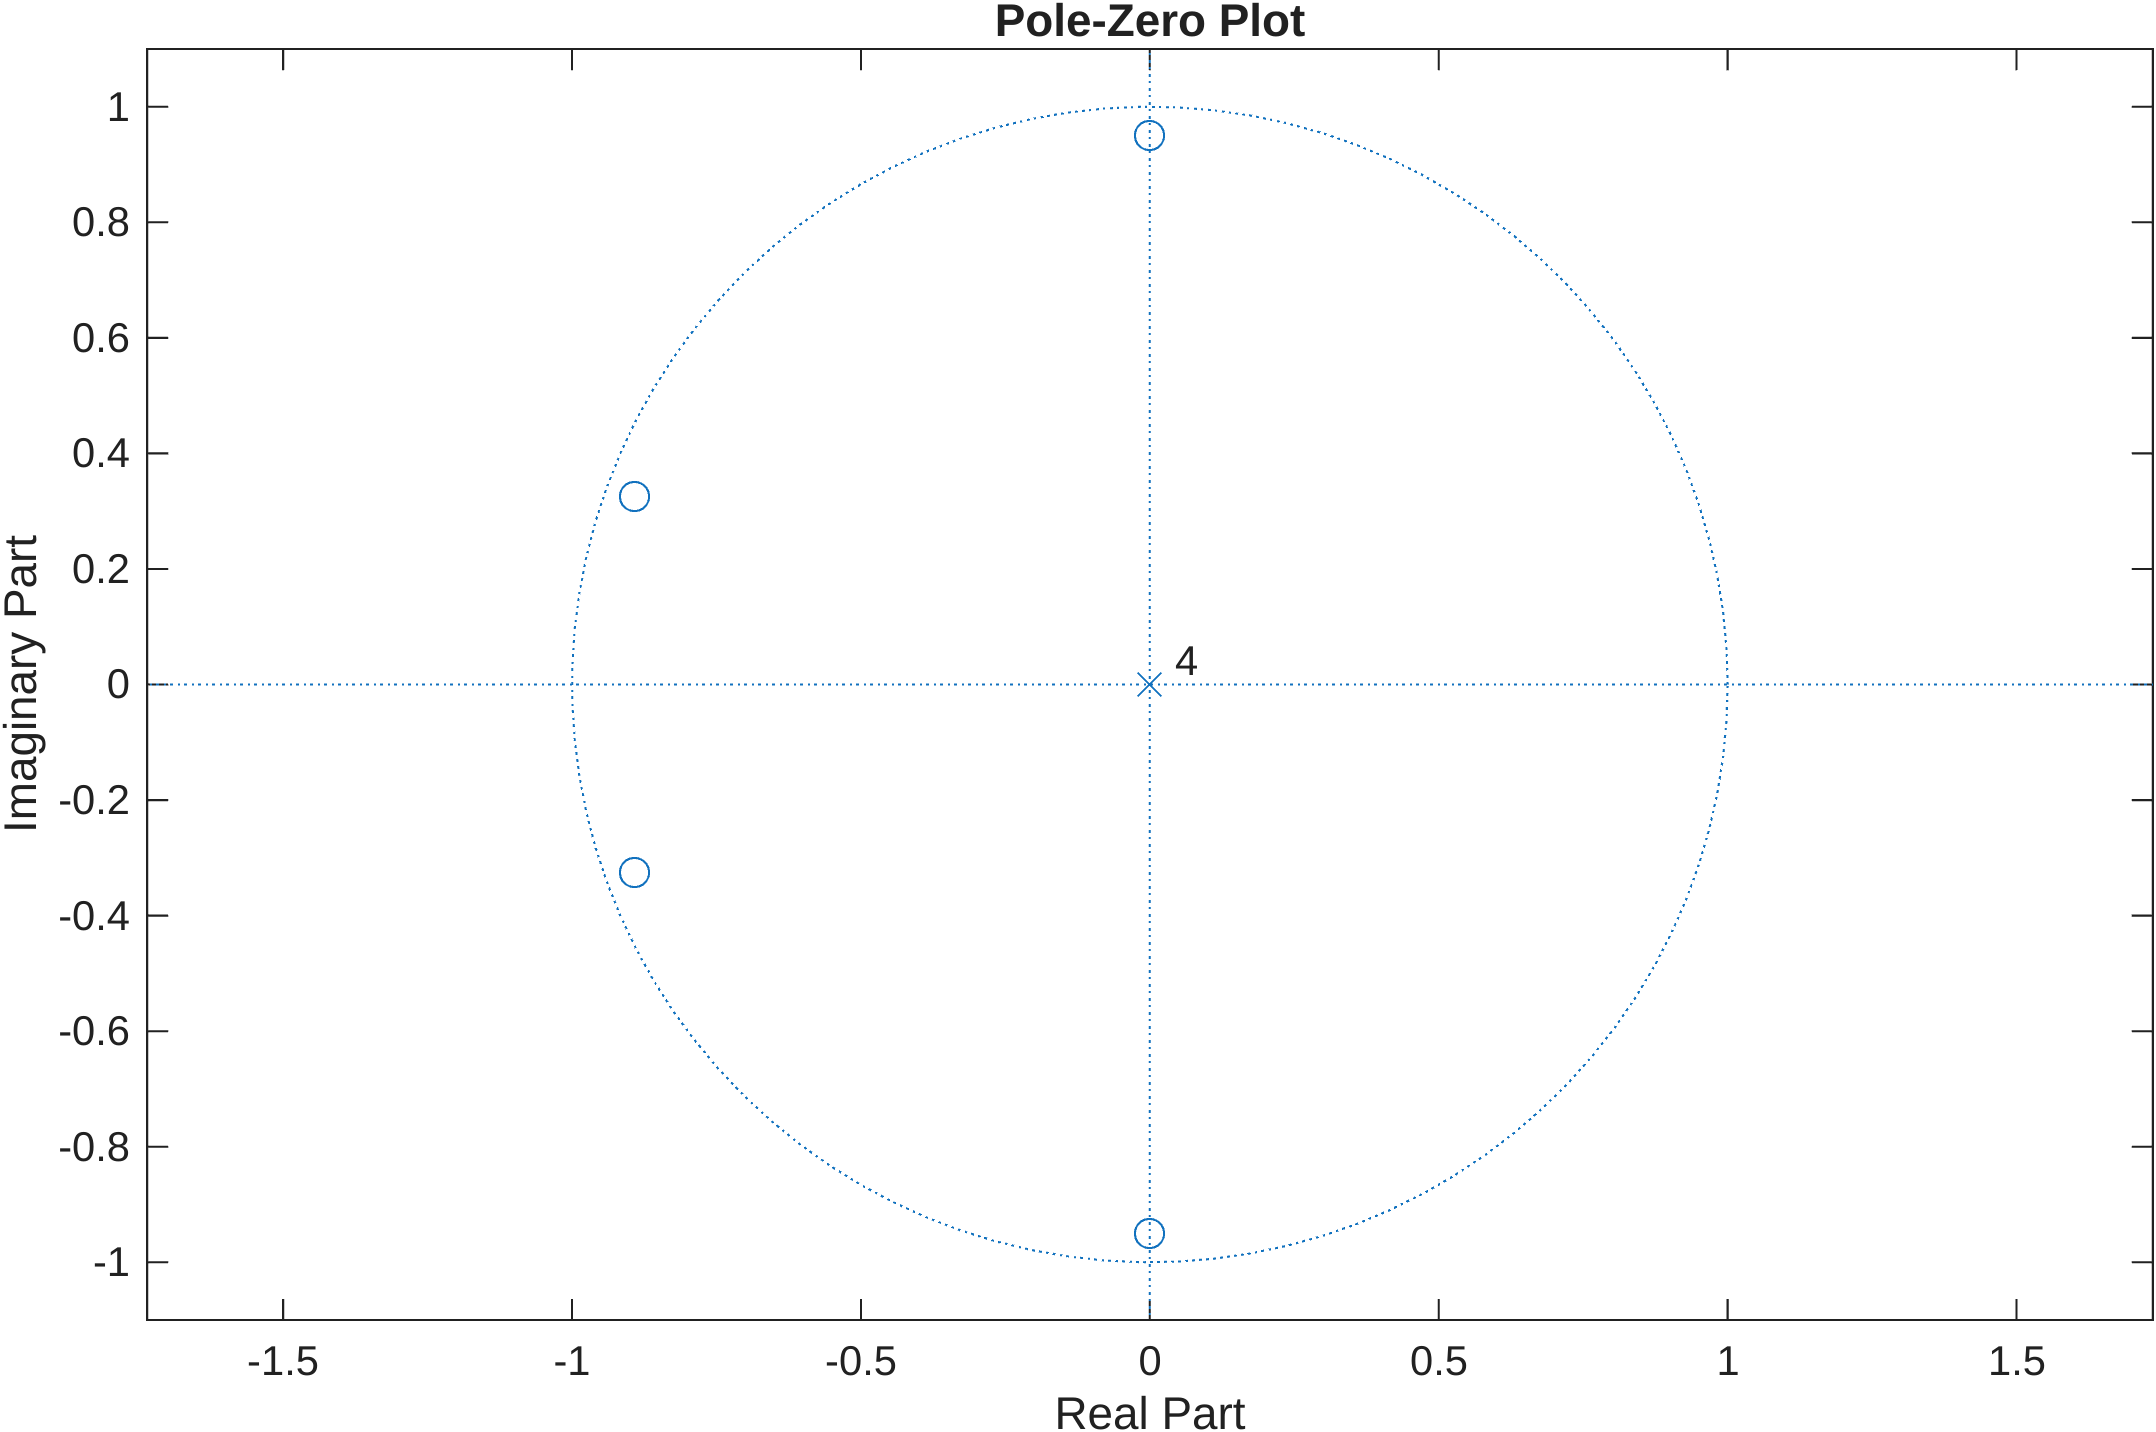
\includegraphics[width=\linewidth]{fig01.png}
    \caption{Plan des pôles et zéros du filtre RIF.}
    \label{fig:zplane_ma}
  \end{subfigure}
  \hfill
  \begin{subfigure}{0.48\linewidth}
    \centering
    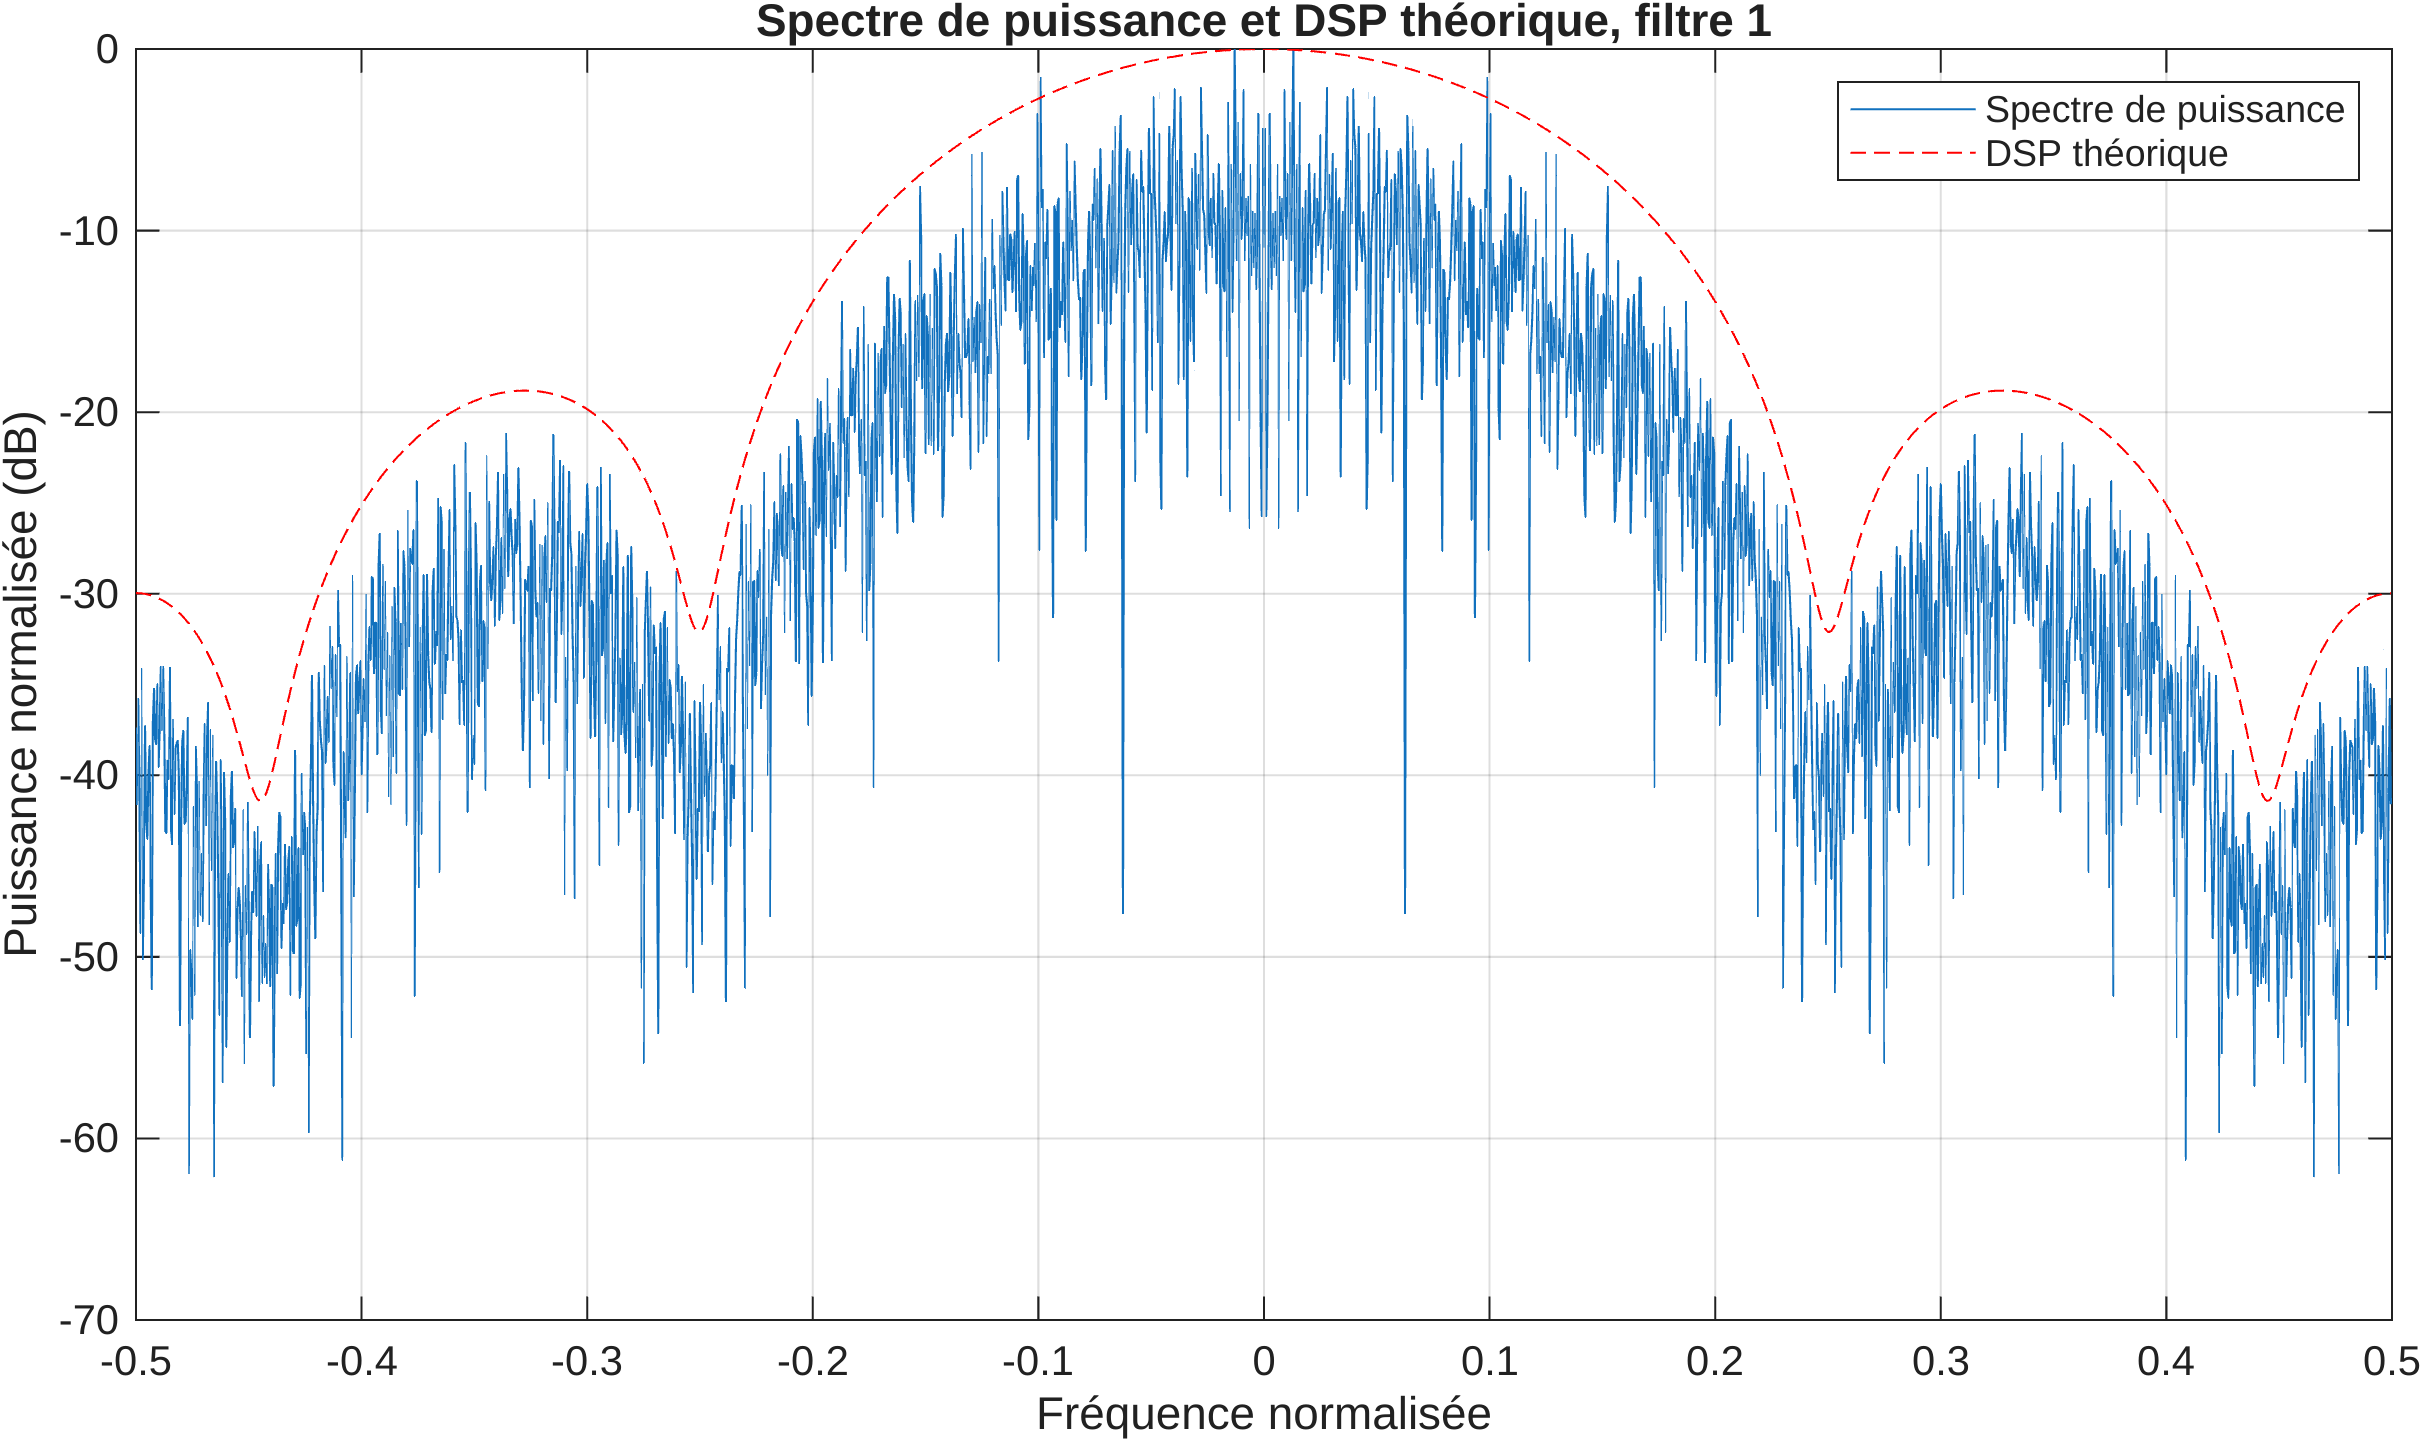
\includegraphics[width=\linewidth]{fig05.png}
    \caption{Périodogramme brut et DSP théorique en dB.}
    \label{fig:ma}
  \end{subfigure}
  \caption{Processus MA(4) : analyse dans le plan en $z$ et densité spectrale de puissance.}
  \label{fig:analyse_ma}
\end{figure}

\subsubsection{2\textsuperscript{de} réalisation}

De manière analogue, le bruit blanc $u(n)$ est désormais filtré par un filtre dont les
quatre pôles, de module $\rho = 0{,}99$, s'écrivent $p_k = r e^{j2\pi\nu_k}$, avec
$\nu_1 = -3/7$, $\nu_2 = -1/3$, $\nu_3 = 1/3$ et $\nu_4 = 3/7$. La disposition des pôles dans le plan complexe est donnée sur la figure~\ref{fig:zplane_ar}. On a donc :
\begin{equation}
  H(z) = \frac{1}{\prod_{k=1}^{4} \left( 1 - p_k\, z^{-1} \right)}
       = \frac{1}{1 + \sum_{i=1}^{4} a_i z^{-i}},
  \qquad
  x(n) = u(n) - \sum_{i=1}^{4} a_i\, x(n-i).
  \label{eq:ar4}
\end{equation}
L'échantillon $x(n)$ dépend désormais de ses quatre échantillons passés : il s'agit d'un
processus autorégressif d'ordre 4.

Contrairement au cas précédent, il s'agit ici d'un filtre RII. Sa
stabilité n'est donc plus garantie : elle est assurée ici car tous les pôles sont à
l'intérieur du cercle unité ($r < 1$). Le processus est alors stationnaire au sens
large, une fois le régime transitoire dû aux conditions initiales écoulé. Les pôles étant
proches du cercle unité, ce régime est plus long que dans le cas MA. Les premiers
échantillons de la réalisation sont donc écartés. La moyenne reste nulle, mais
l'autocorrélation n'est plus nulle au-delà d'un certain rang : elle vérifie, $r_x(k) = -\sum_{i=1}^{4} a_i\, r_x(k-i)$ pour $k \geq 1$.

Par analogie avec \eqref{eq:dsp_ma}, la densité spectrale de puissance s'écrit :
\begin{equation}
  S_x(\nu) = \frac{\sigma_u^2}{\left| A\!\left(e^{j2\pi\nu}\right) \right|^2},
  \qquad A(z) = 1 + \sum_{i=1}^{4} a_i z^{-i}.
  \label{eq:dsp_ar}
\end{equation}
Les creux du cas MA laissent place à des pics de résonance en $\nu_3 = 1/3$ et
$\nu_4 = 3/7$, visibles sur la figure~\ref{fig:ar}. La comparaison directe entre les spectres d'amplitude des filtres RIF et RII est présentée sur la figure~\ref{fig:spectres_amp}.

\begin{figure}[htbp]
  \centering
  \begin{subfigure}{0.48\linewidth}
    \centering
    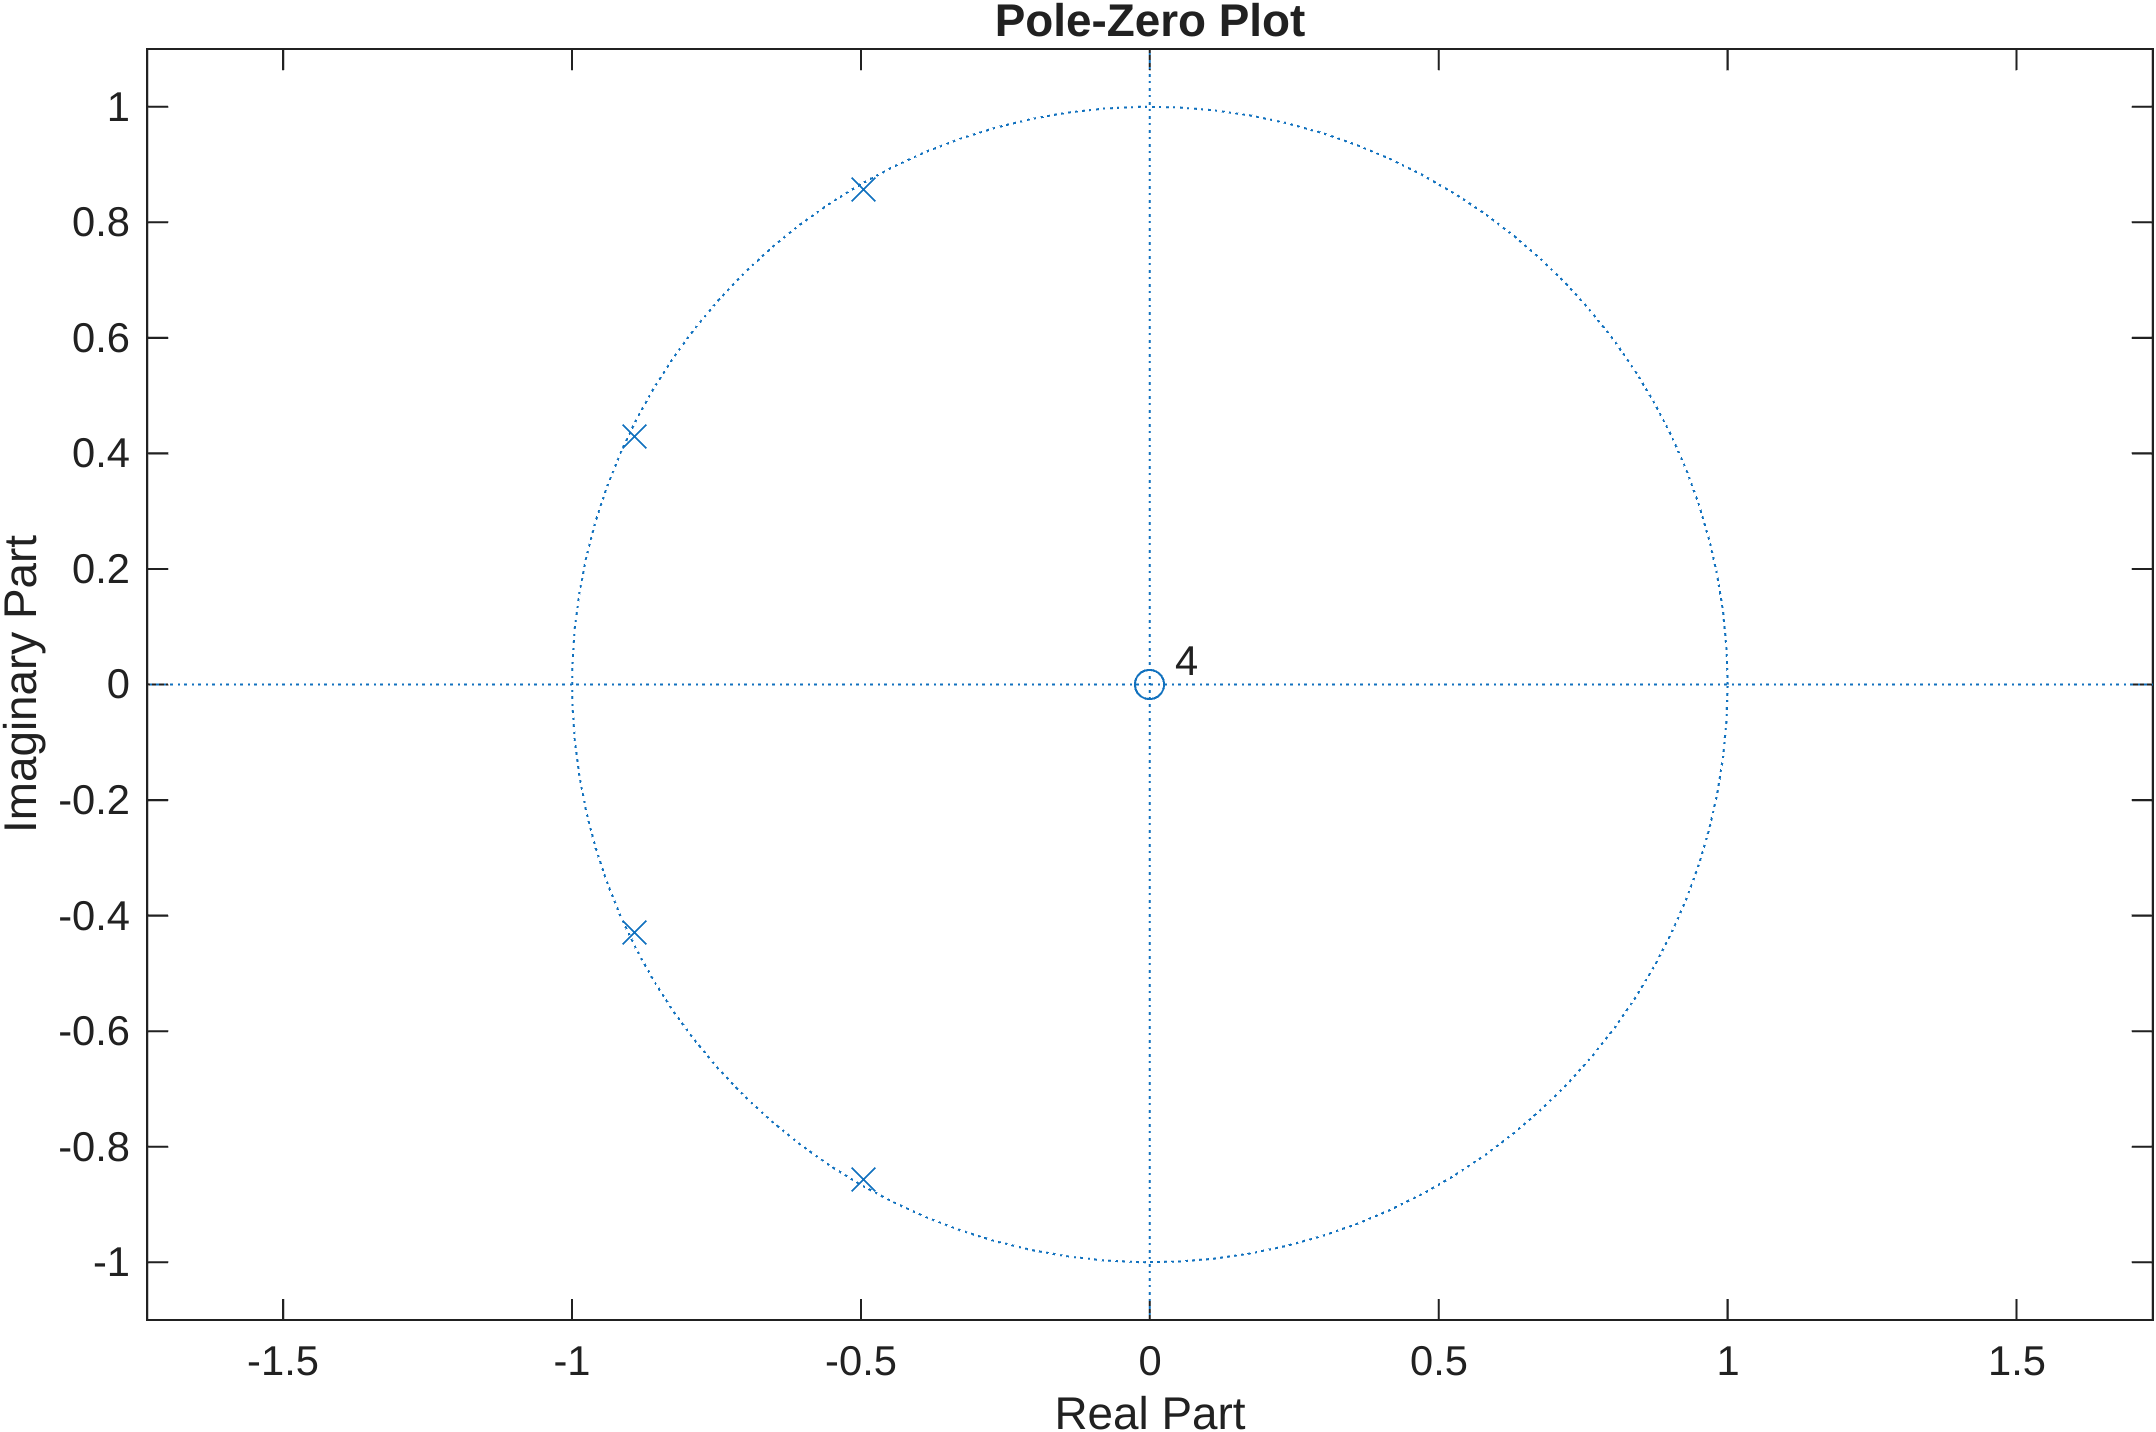
\includegraphics[width=\linewidth]{fig03.png}
    \caption{Plan des pôles et zéros du filtre RII.}
    \label{fig:zplane_ar}
  \end{subfigure}
  \hfill
  \begin{subfigure}{0.48\linewidth}
    \centering
    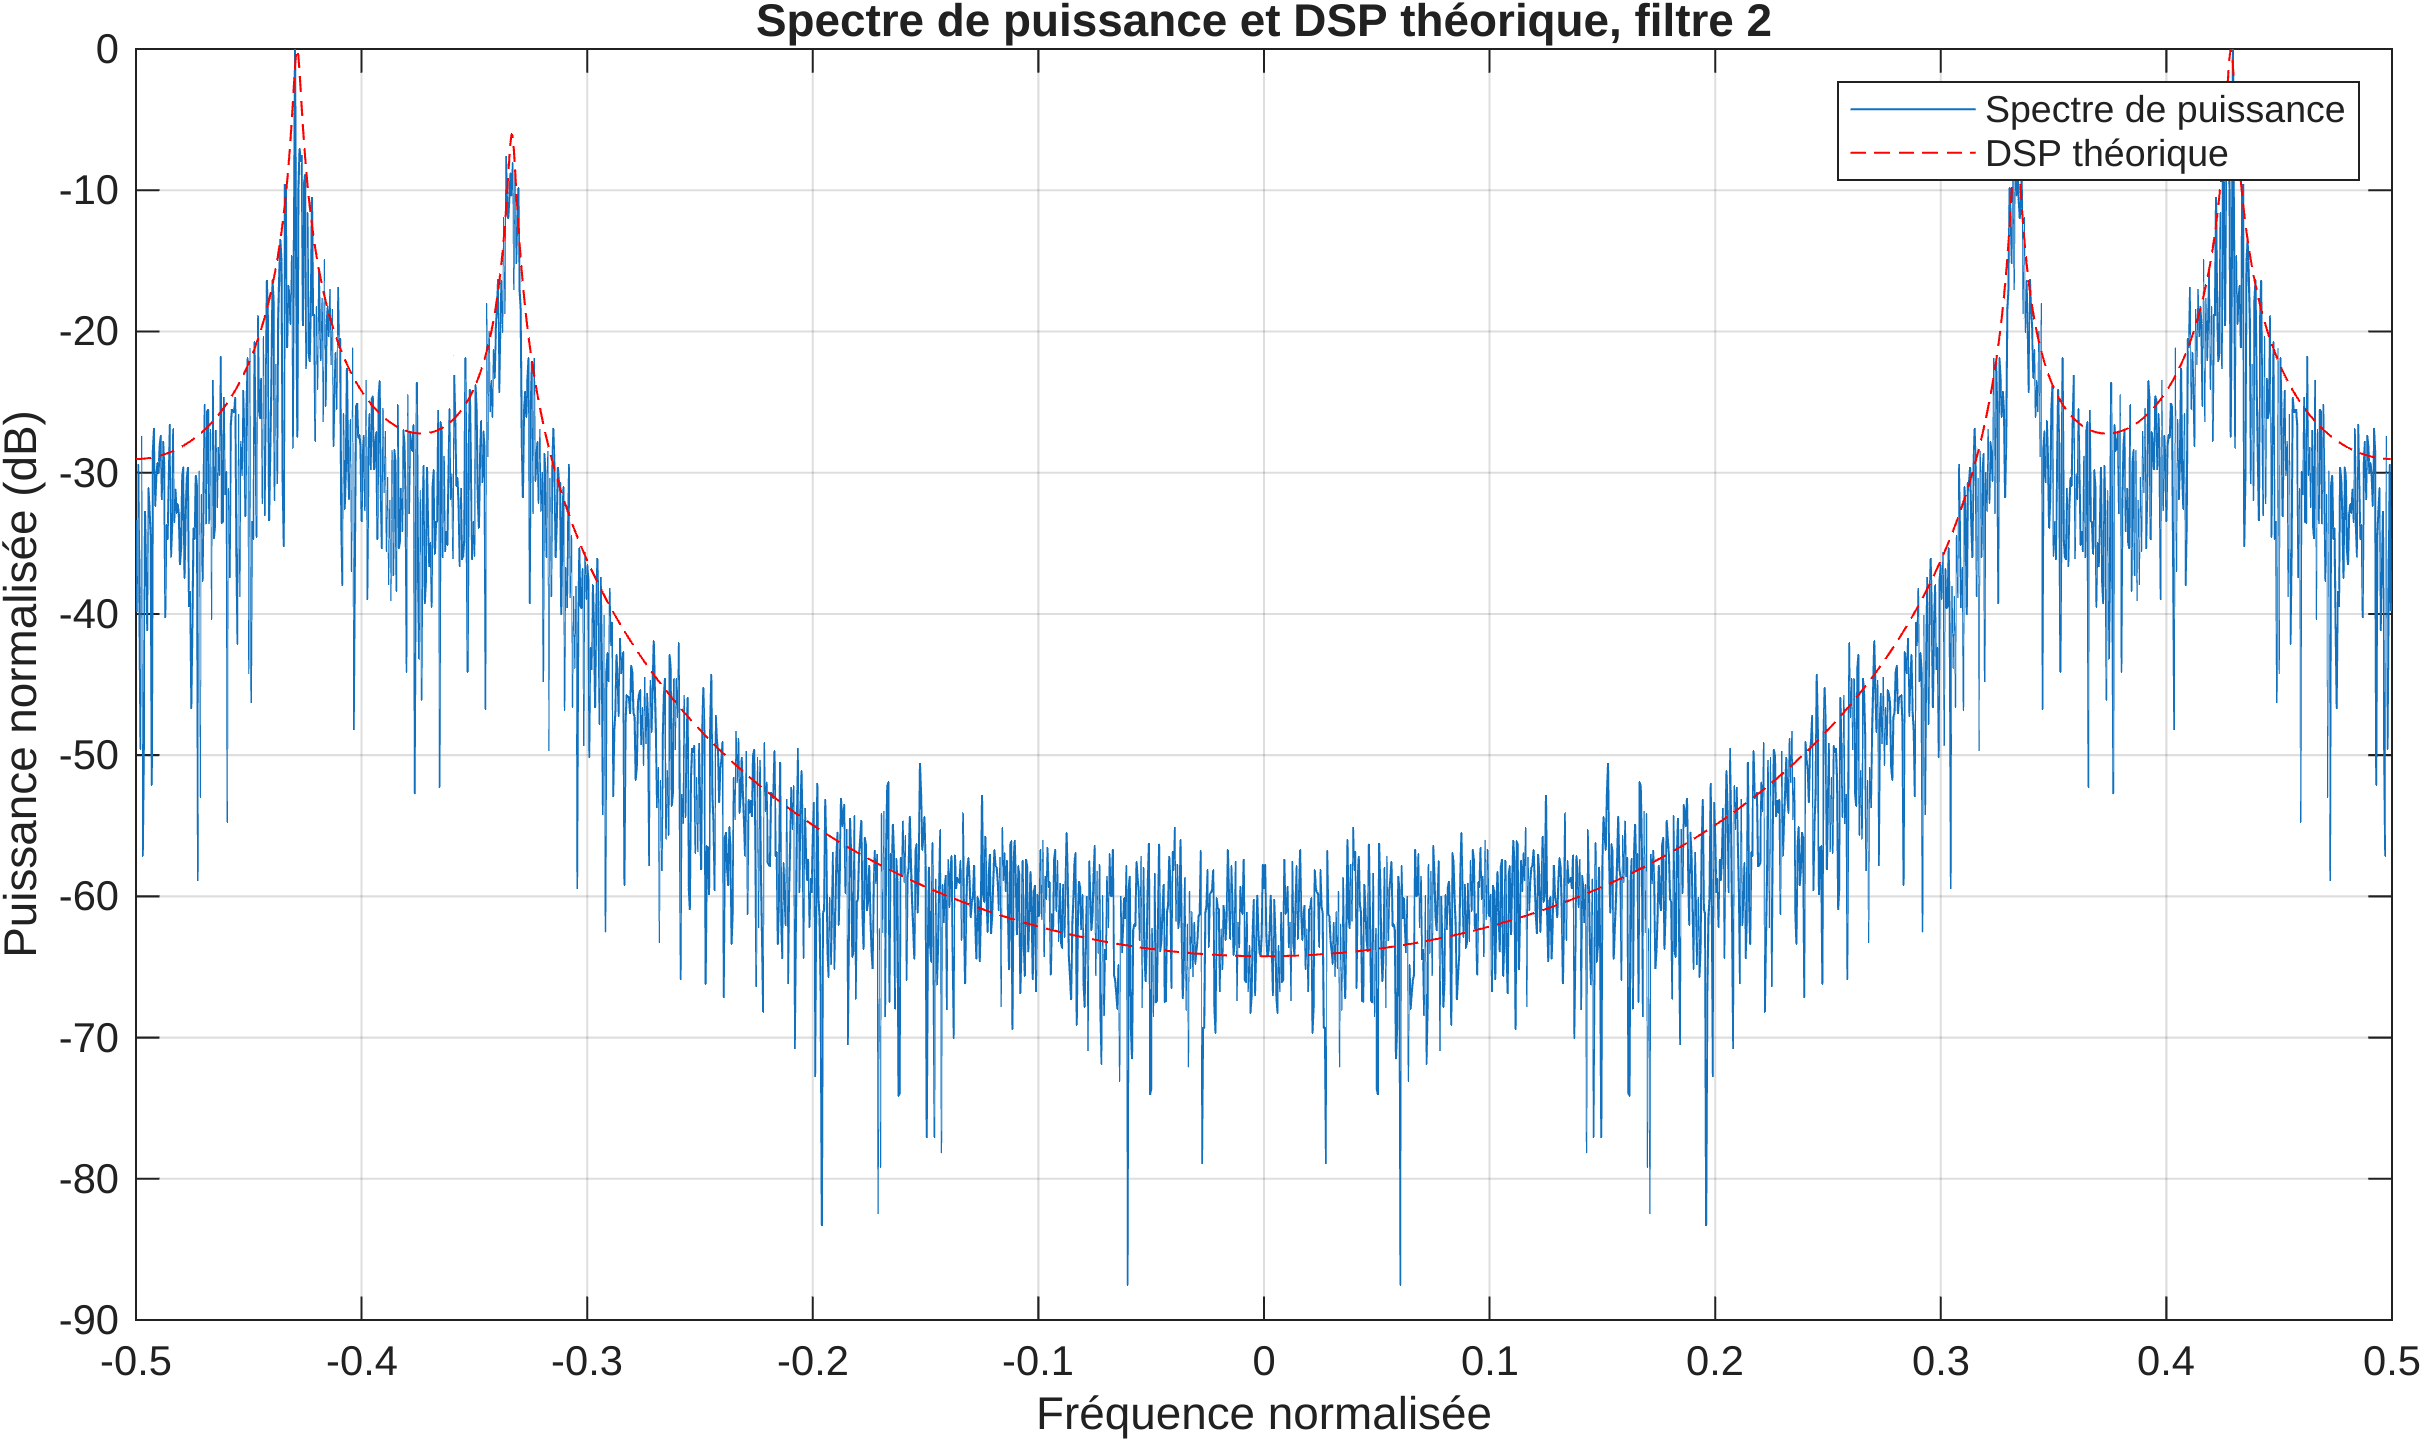
\includegraphics[width=\linewidth]{fig06.png}
    \caption{Périodogramme brut et DSP théorique en dB.}
    \label{fig:ar}
  \end{subfigure}
  \caption{Processus AR(4) : analyse dans le plan en $z$ et densité spectrale de puissance.}
  \label{fig:analyse_ar}
\end{figure}

\subsubsection{Représentations temporelles}

\begin{figure}[H]
  \centering
  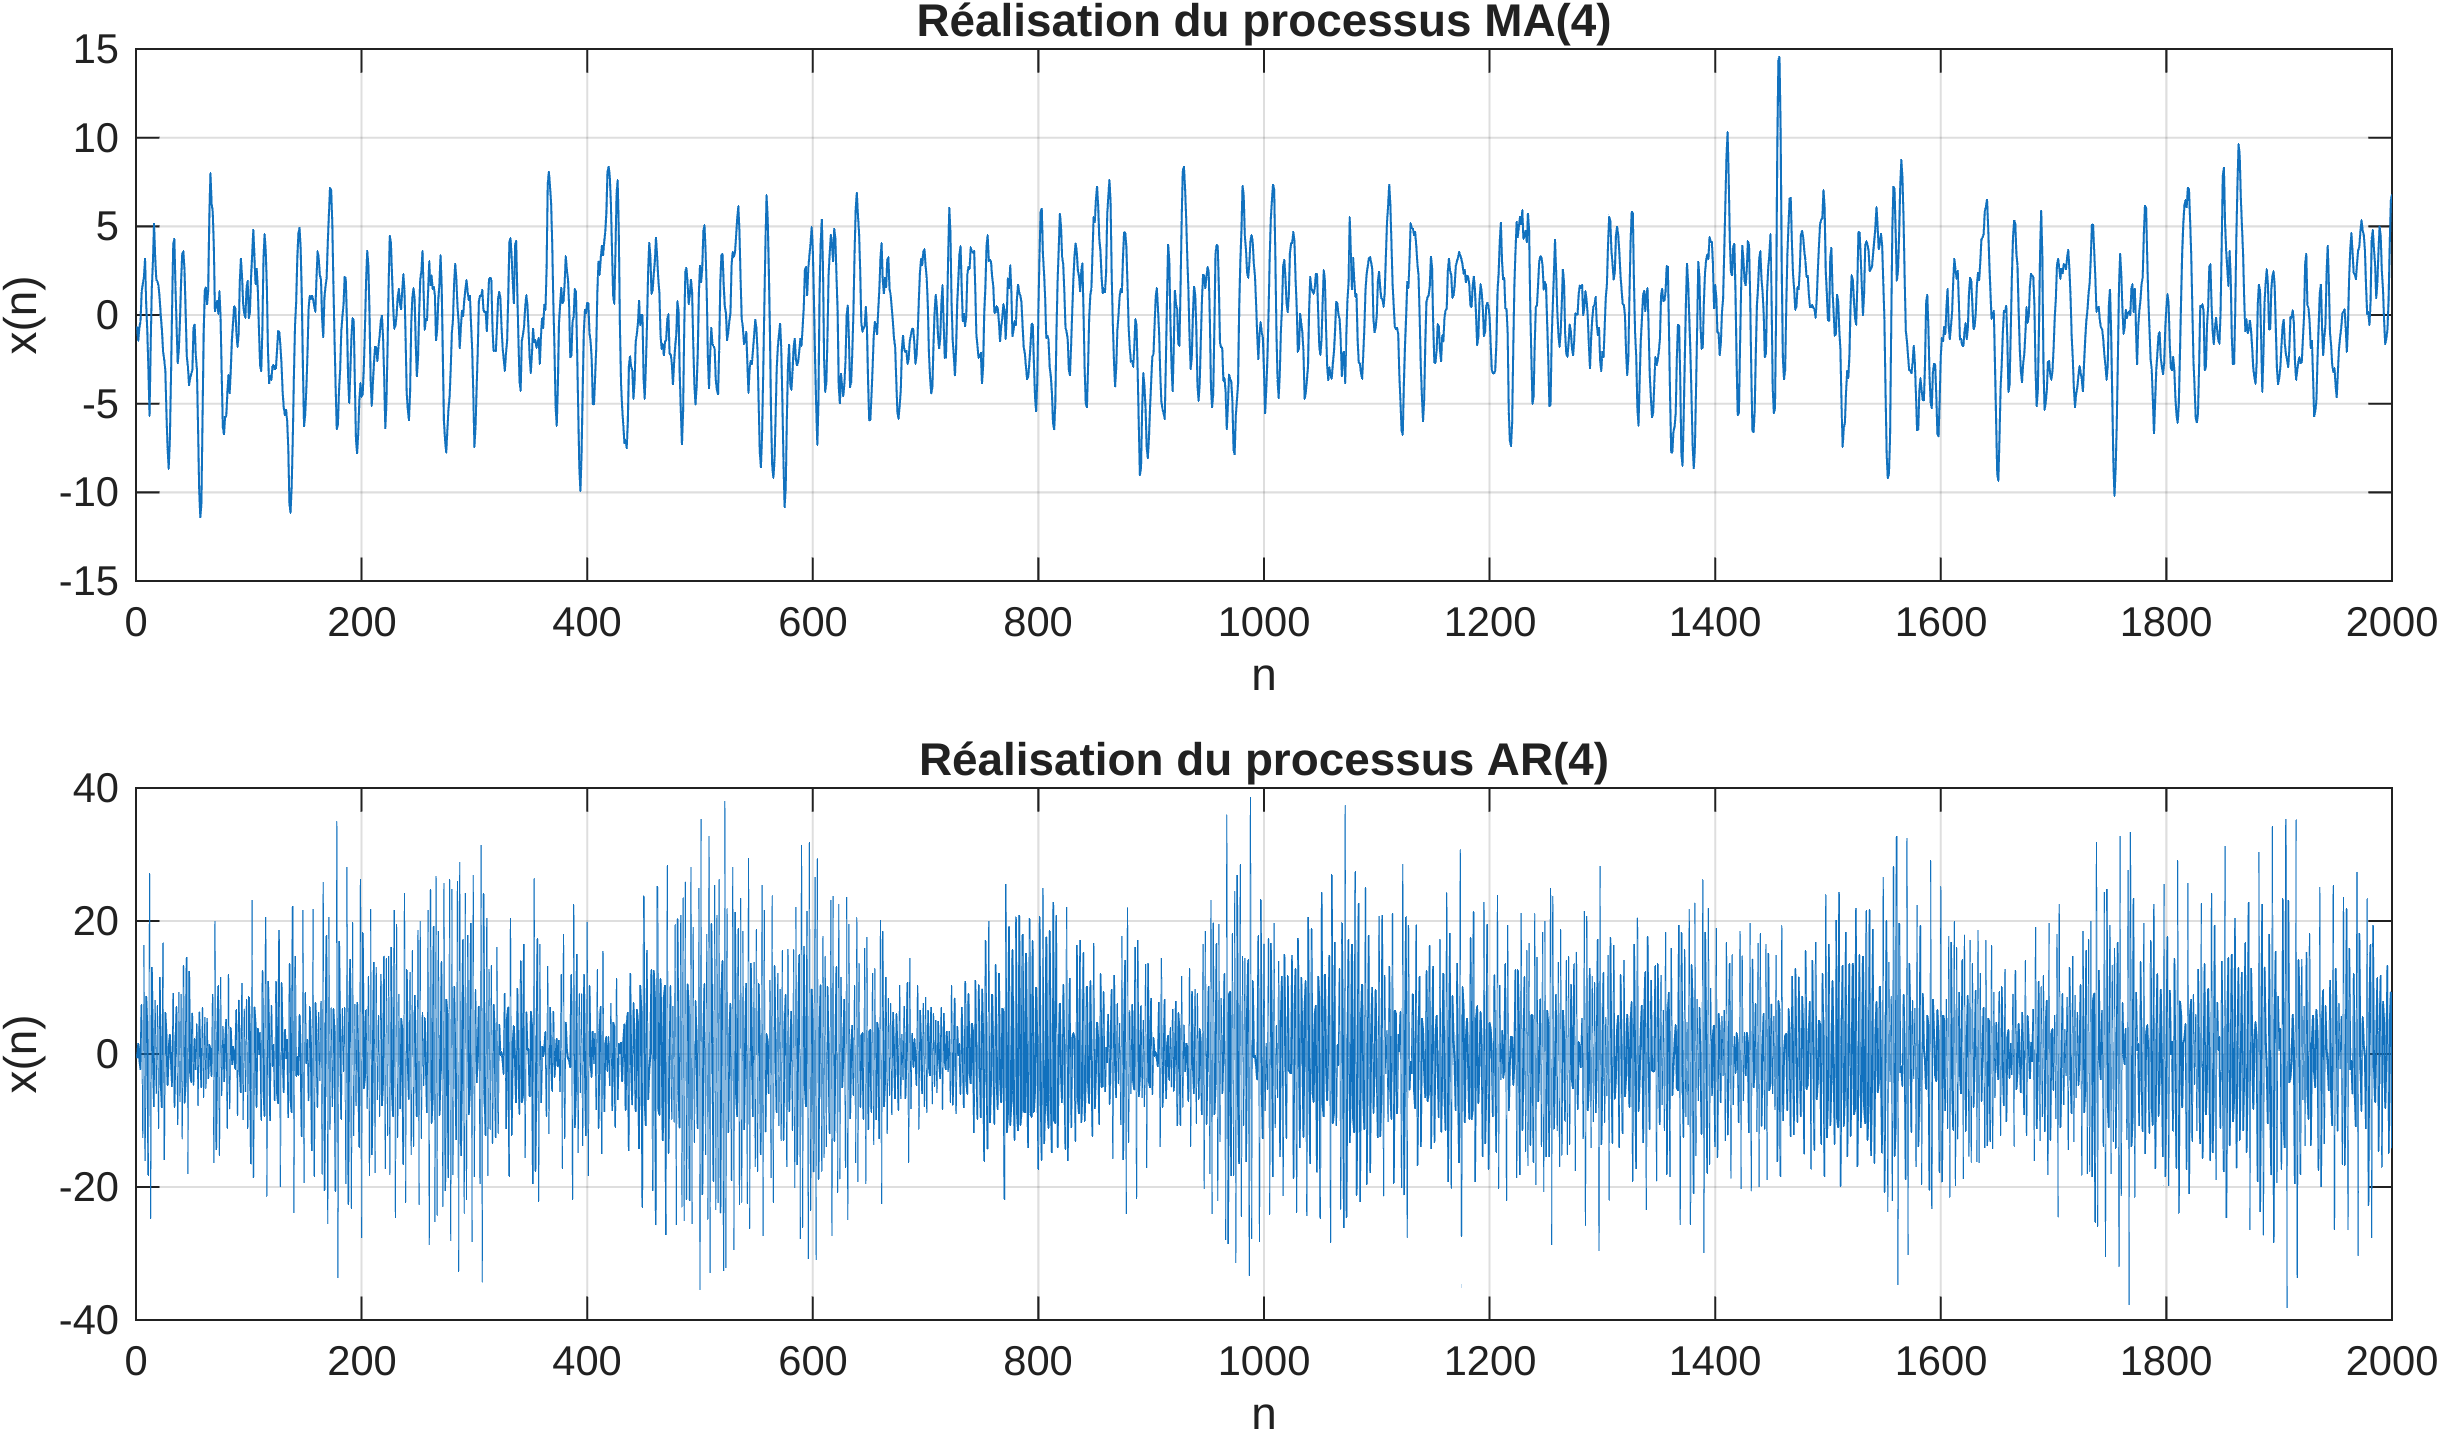
\includegraphics[width=0.85\linewidth]{fig04.png}
  \caption{Réalisations temporelles des processus MA(4) et AR(4) ($N = 2000$ échantillons).}
  \label{fig:temporelles}
\end{figure}

\subsubsection{Périodogrammes}
Soit $I$ un périodogramme tel que : \\
\begin{equation}
    I(f) = \frac{1}{N} \left| \sum_{n=0}^{N-1} x(n) e^{-j 2 \pi f n} \right|^2
    \label{eq:periodogramme_standard}
\end{equation}
\\
    \indent Périodogramme de Daniell:
\\
    On formule de cette expression le périodogramme de Daniell, il consiste en une moyenne mobile de taille $(2m + 1)$ dans le domaine fréquentiel du périodogramme standard ci-dessus :
\\
\begin{equation}
    \hat{S}_{\text{Daniell}}(f_k) = \frac{1}{2m + 1} \sum_{j = -m}^{m} I(f_{k + j})
\end{equation}
Pour choisir la taille de fenêtre optimale afin de réduire au maximum la variance de l'estimateur sans déformer le spectre, on utilise la formule théorique exacte de non-distorsion spectrale pour un périodogramme de Daniell : \\ \\
\begin{equation}
    {M}{\Delta f}<{\Delta_{FWHM}}
\end{equation}
où ${M}$ est la largeur de la fenêtre de lissage, ${\Delta f}$ est le pas fréquentiel et $\Delta_{FWHM}$ est la largeur à mi-hauteur de la variation spectrale la plus étroite du filtre.

Dans le cas de nos deux processus on a :
    $$\Delta f = \frac{fe}{N} = \frac{1}{N}$$
    où $N$ est la longueur de la séquence temporelle,
\begin{equation}
    \Delta_{FWHM,MA}=\frac{1-R}{\pi R}
\end{equation}
\begin{equation}
    \Delta_{FWHM,AR}=\frac{1-r}{\pi r}
\end{equation}

Application numérique :
    $$\Delta_{FWHM,MA} \approx 0{,}0167$$
    $$\Delta_{FWHM,AR} \approx 0{,}0032$$

Donc :
    $$M_{MA}<33{,}5$$
    $$M_{AR}<6{,}4$$
On choisit alors :
    $$m_{MA} = 16$$
    $$m_{AR} = 2$$

\begin{figure}[htbp]
  \centering
  \begin{subfigure}{0.49\linewidth}
    \centering
    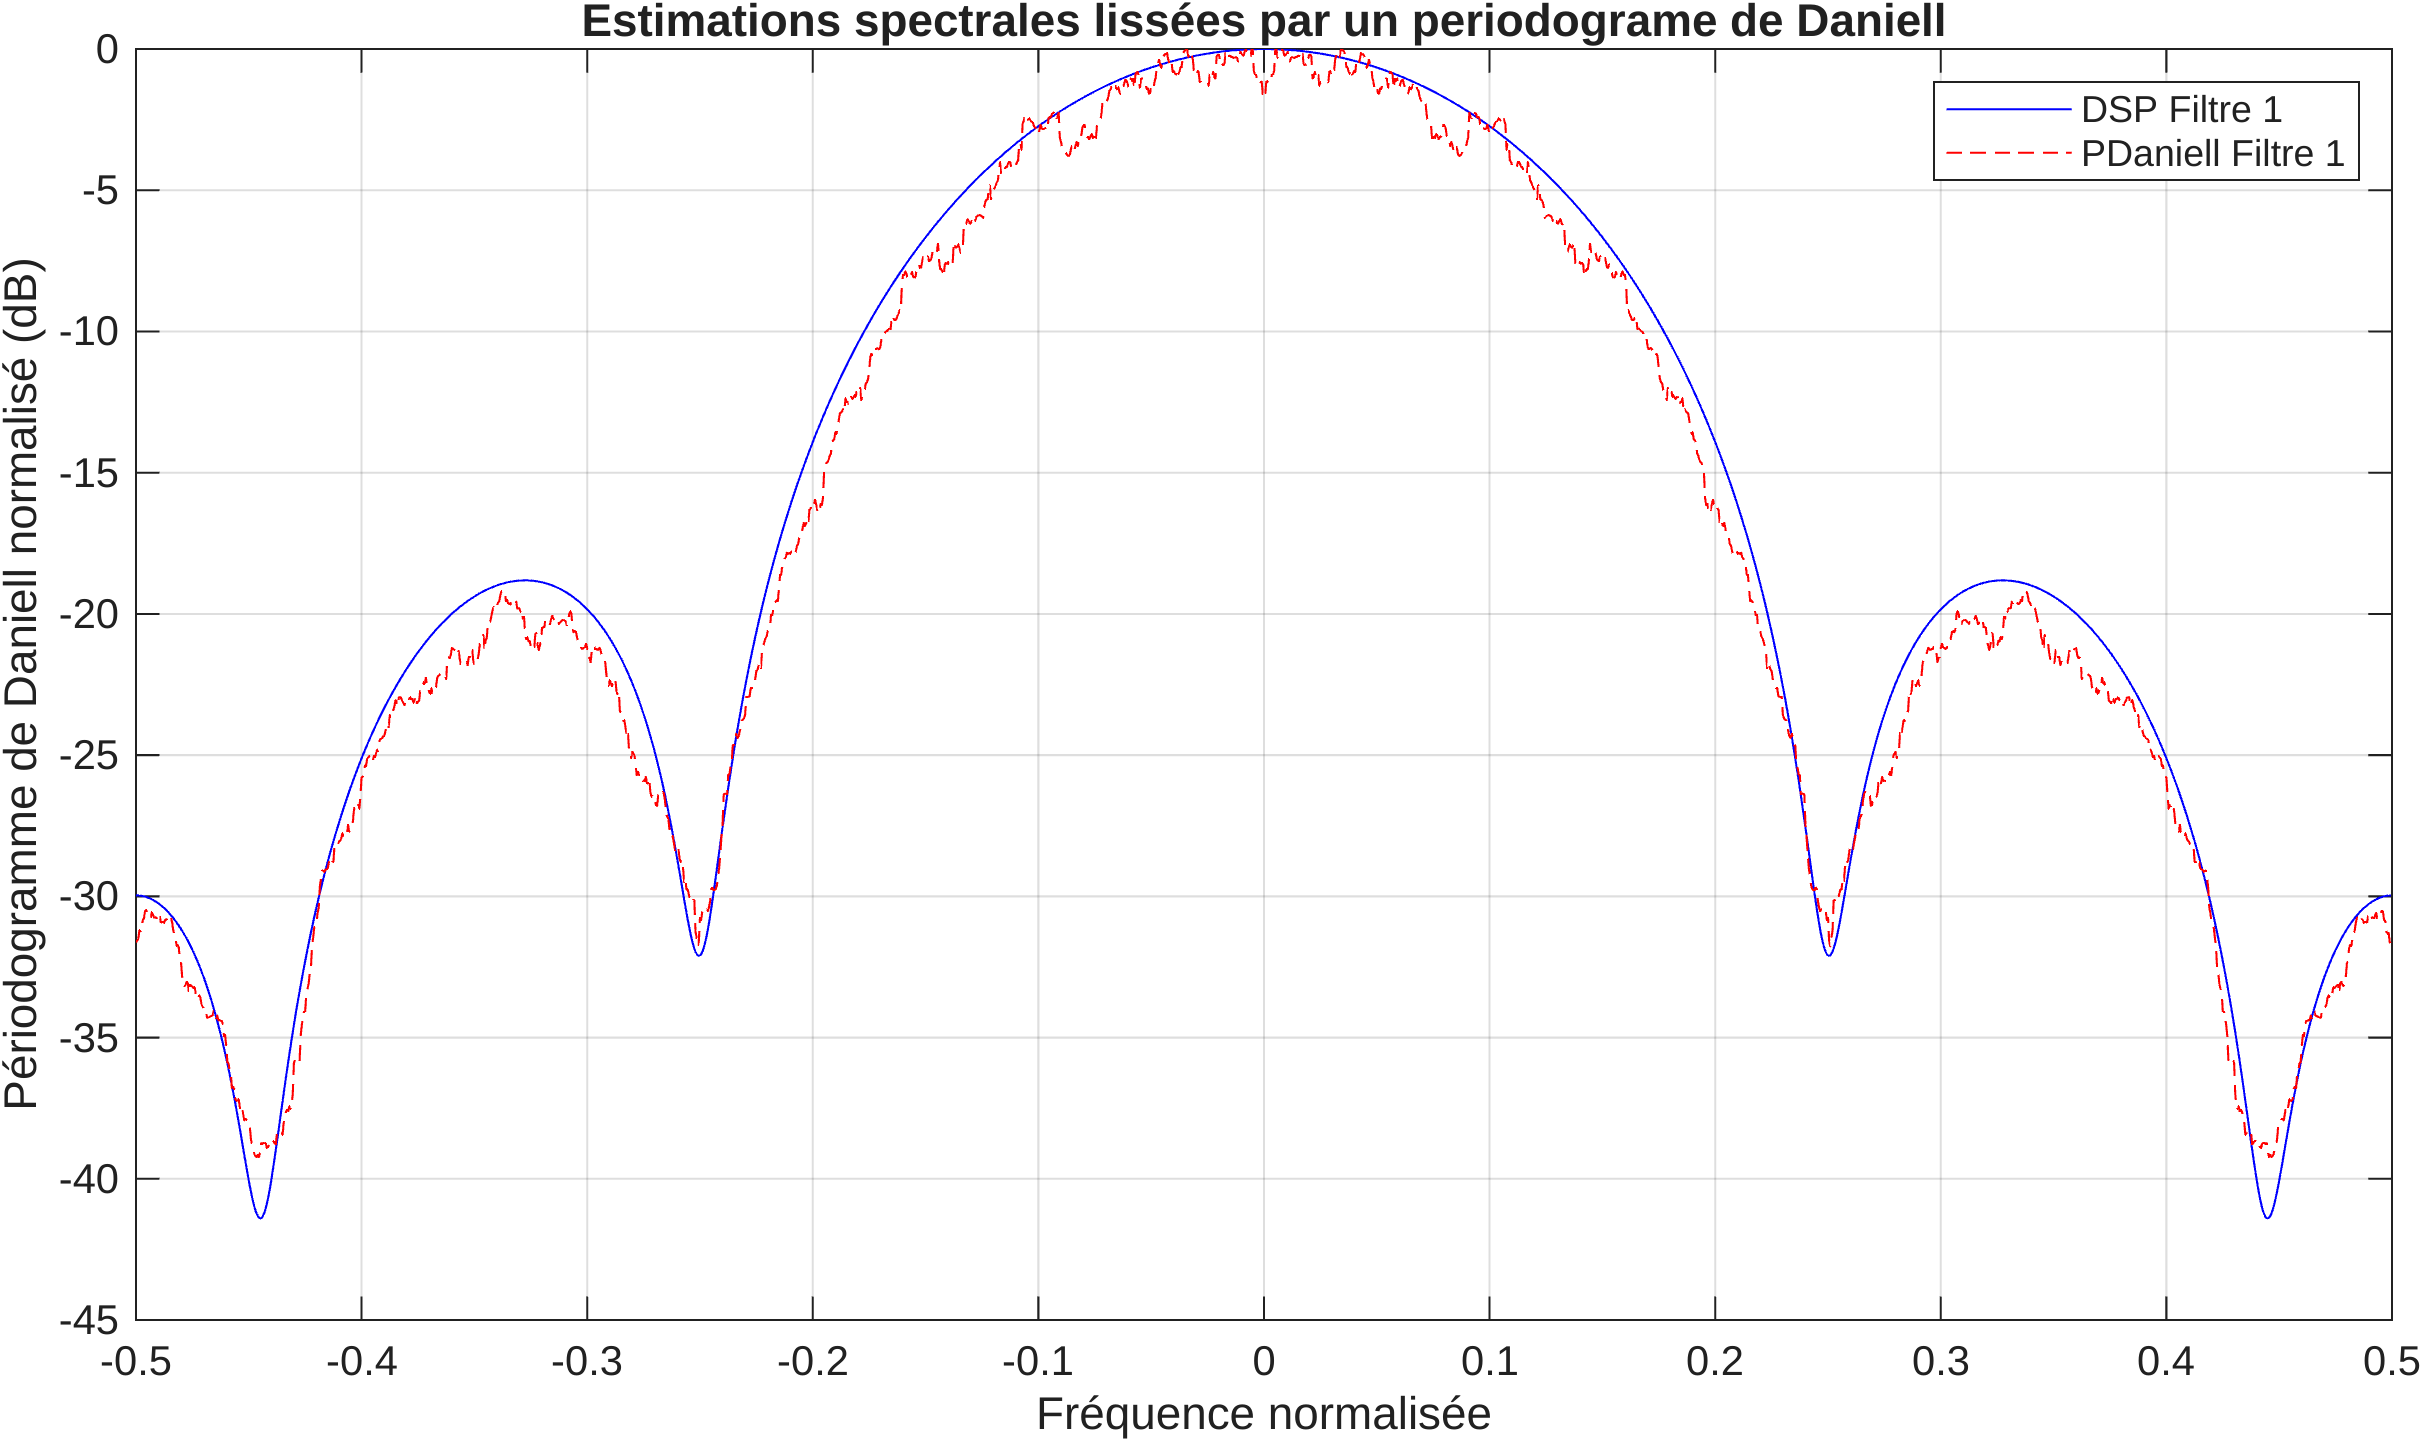
\includegraphics[width=\linewidth]{fig07.png}
    \caption{Processus MA ($m_{\text{MA}} = 16$)}
    \label{fig:daniell_ma}
  \end{subfigure}
  \hfill
  \begin{subfigure}{0.49\linewidth}
    \centering
    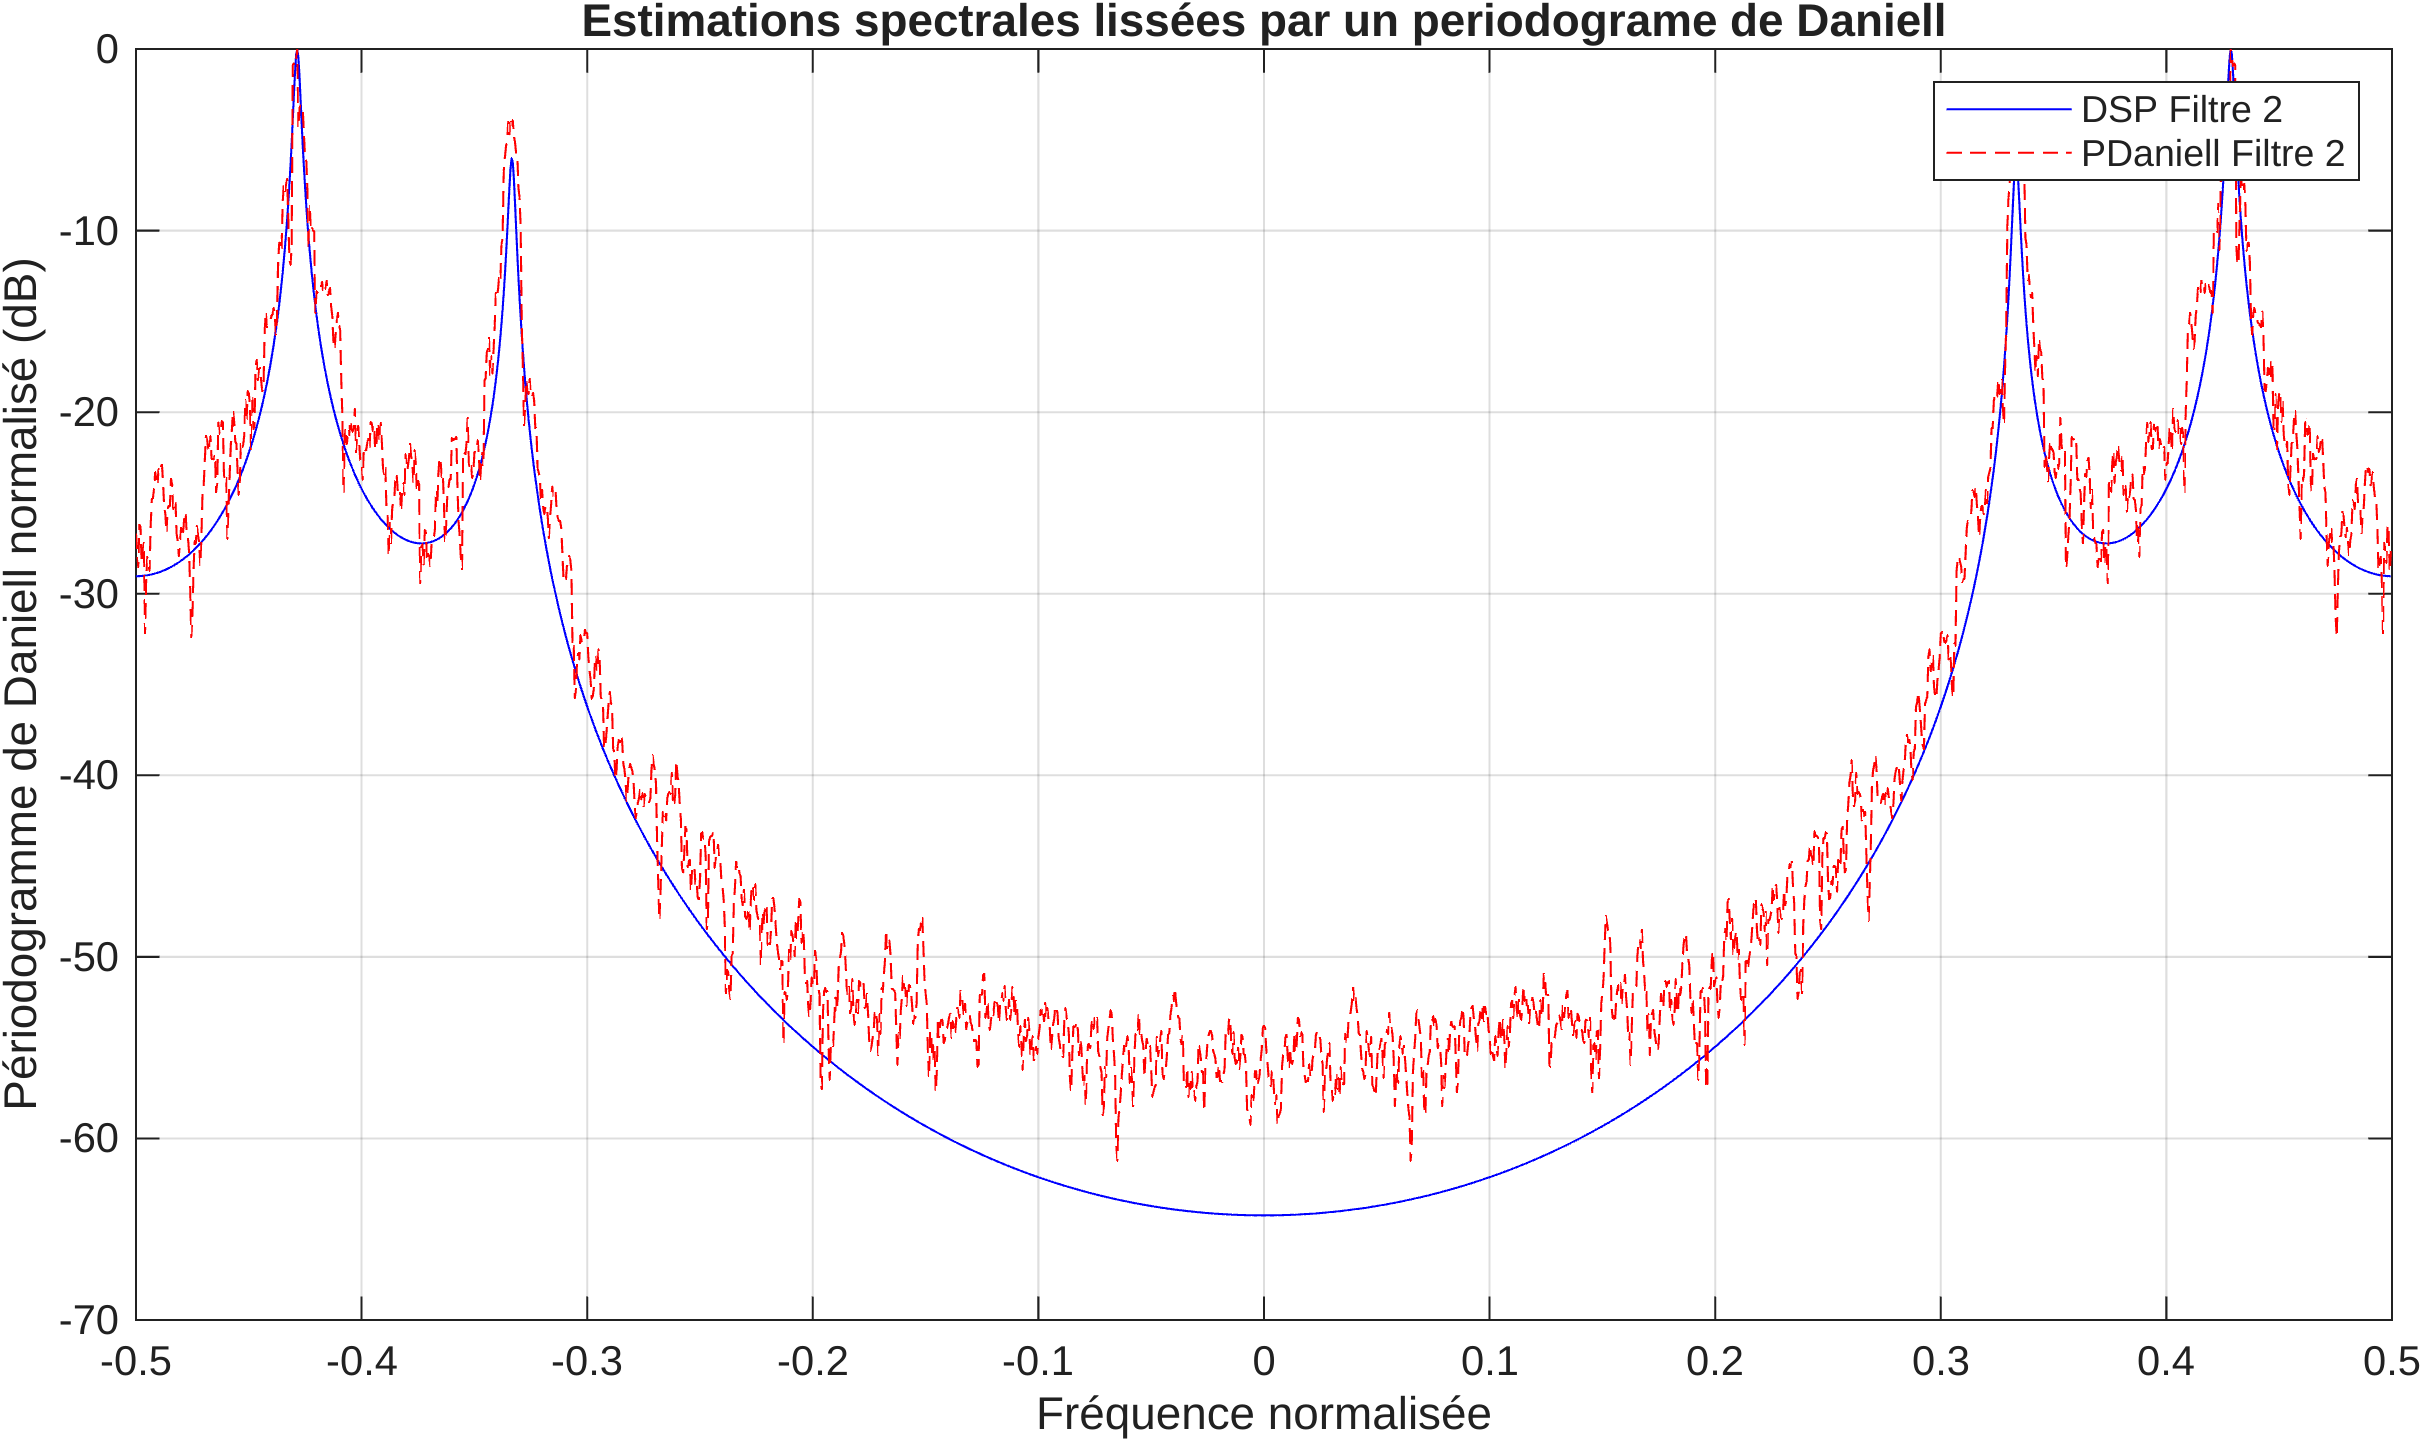
\includegraphics[width=\linewidth]{fig08.png}
    \caption{Processus AR ($m_{\text{AR}} = 2$)}
    \label{fig:daniell_ar}
  \end{subfigure}
  \caption{Périodogrammes de Daniell pour les processus MA et AR.}
  \label{fig:daniell}
\end{figure}

Ce calcul met en évidence la limite intrinsèque du périodogramme de Daniell (figure~\ref{fig:daniell}) :\\
\begin{equation}
    \operatorname{Var}(\hat{S}_{\text{Daniell}}) \approx \frac{1}{2m+1} S_x^2
\end{equation}

    - Pour le processus à variations spectrales lentes (figure~\ref{fig:daniell_ma}), la fenêtre admissible ($m = 16$) permet un lissage efficace, la variance est divisée par 33 tout en respectant les conditions de non-distorsion.\\
    \indent - Pour le processus à variations spectrales rapides (figure~\ref{fig:daniell_ar}), la théorie bride la taille de fenêtre à une valeur très faible ($m = 2$). L'estimateur préserve la forme du pic mais ne peut réduire la variance que d'un facteur 5, laissant le tracé fortement impacté par le bruit.\\
    \indent - Daniell illustre donc parfaitement le dilemme : on ne peut pas lisser efficacement le bruit sur un spectre très résonant sans en détruire les extrema.\\

Périodogramme de Bartlett :
\\
Le principe de ce périodogramme consiste à découper le signal en $K$ blocs de longueur $M$, tels que $K = \frac{N}{M}$, de calculer le périodogramme $I$ défini en \eqref{eq:periodogramme_standard} sur chacun des blocs, puis de faire la moyenne arithmétique sur les $K$ périodogrammes, d'où les formules suivantes :

\begin{equation}
    I_i(f) = \frac{1}{M} \left| \sum_{n=0}^{M-1} x_i(n) e^{-j 2 \pi f n} \right|^2
\end{equation}
\begin{equation}
    \hat{S}_{\text{Bartlett}}(f) = \frac{1}{K} \sum_{i=1}^{K} I_i(f)
\end{equation}

D'une manière similaire, pour le choix de la longueur des $K$ blocs, la condition de non-distorsion spectrale pour un périodogramme de Bartlett impose :
\begin{equation}
    \Delta f < {\Delta}_{FWHM}
    \iff M > \frac{1}{{\Delta}_{FWHM}}
\end{equation}
Application numérique :
\begin{equation}
    M_{MA} \ge 60 \implies M_{MA,choisi} = 80
\end{equation}
\begin{equation}
    M_{AR} \ge 313 \implies M_{AR, choisi} = 400
\end{equation}
\\
Dans le cas du périodogramme de Bartlett on a :
\begin{equation}
    \operatorname{Var}(\hat{S}_{\text{Bartlett}}) \approx \frac{1}{K} S_x^2
\end{equation}

Ainsi on a :
$$K_{MA} = 25$$  $$K_{AR} = 5$$

\begin{figure}[htbp]
  \centering
  \begin{subfigure}{0.49\linewidth}
    \centering
    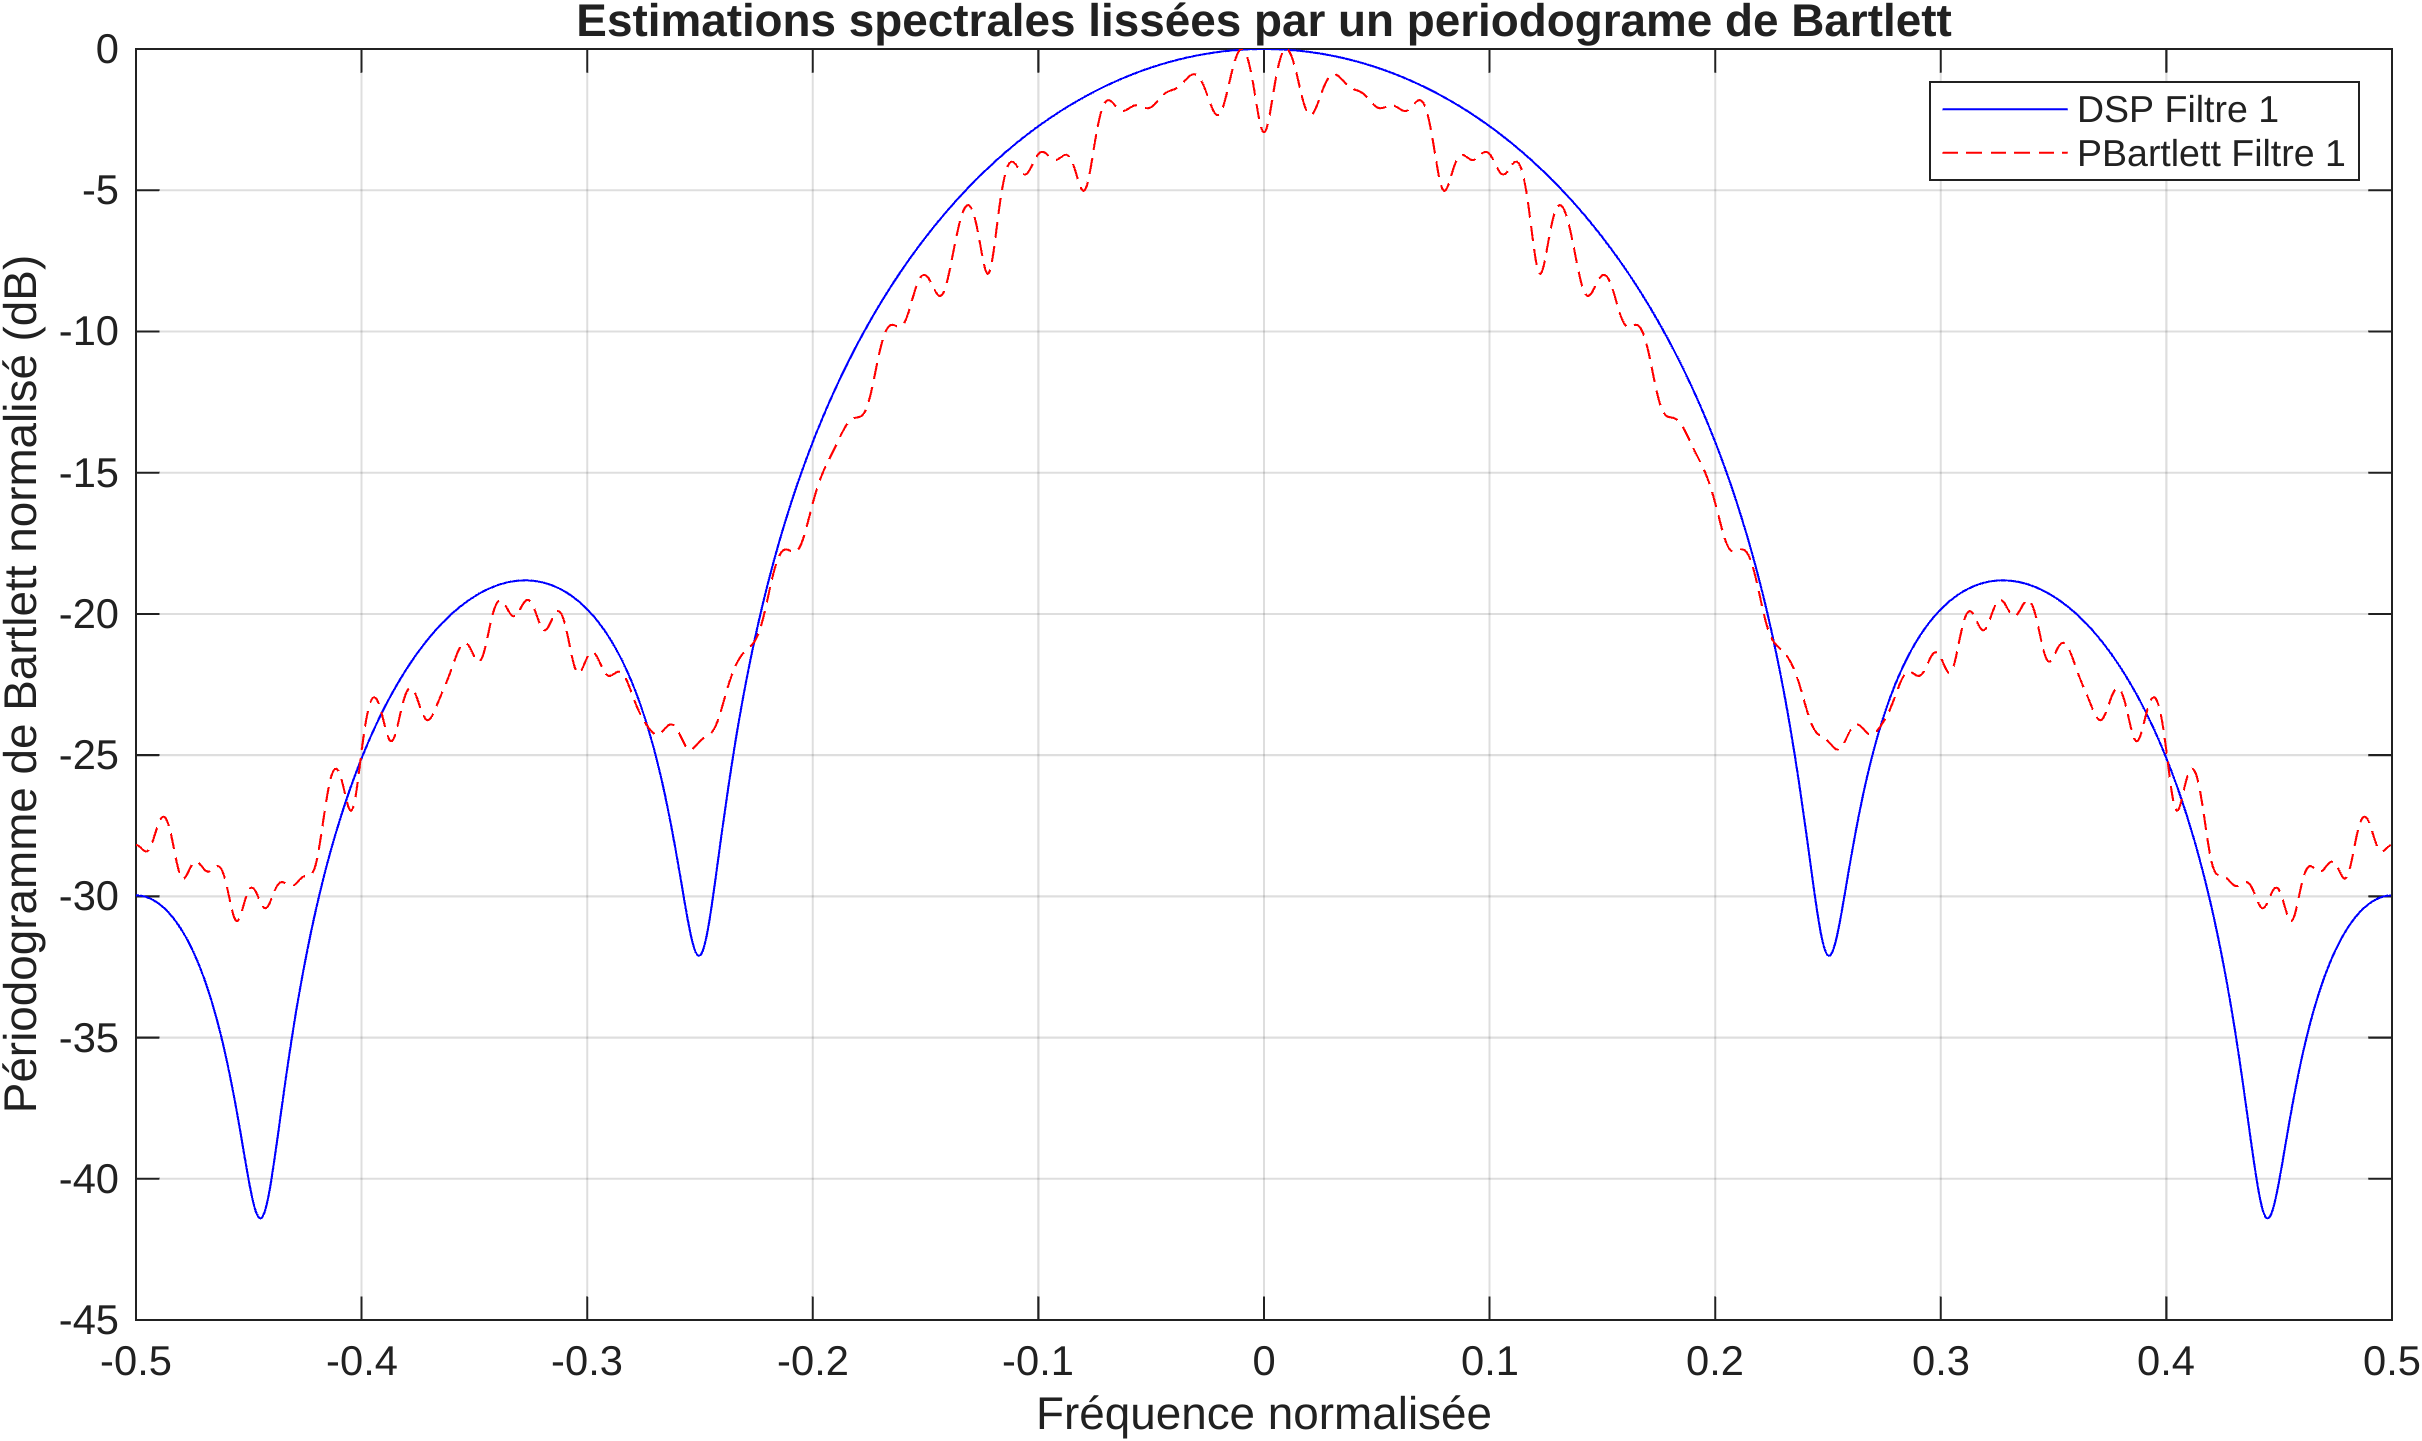
\includegraphics[width=\linewidth]{fig09.png}
    \caption{Processus MA ($M_{\text{MA}} = 80$, $K = 25$)}
    \label{fig:bartlett_ma}
  \end{subfigure}
  \hfill
  \begin{subfigure}{0.49\linewidth}
    \centering
    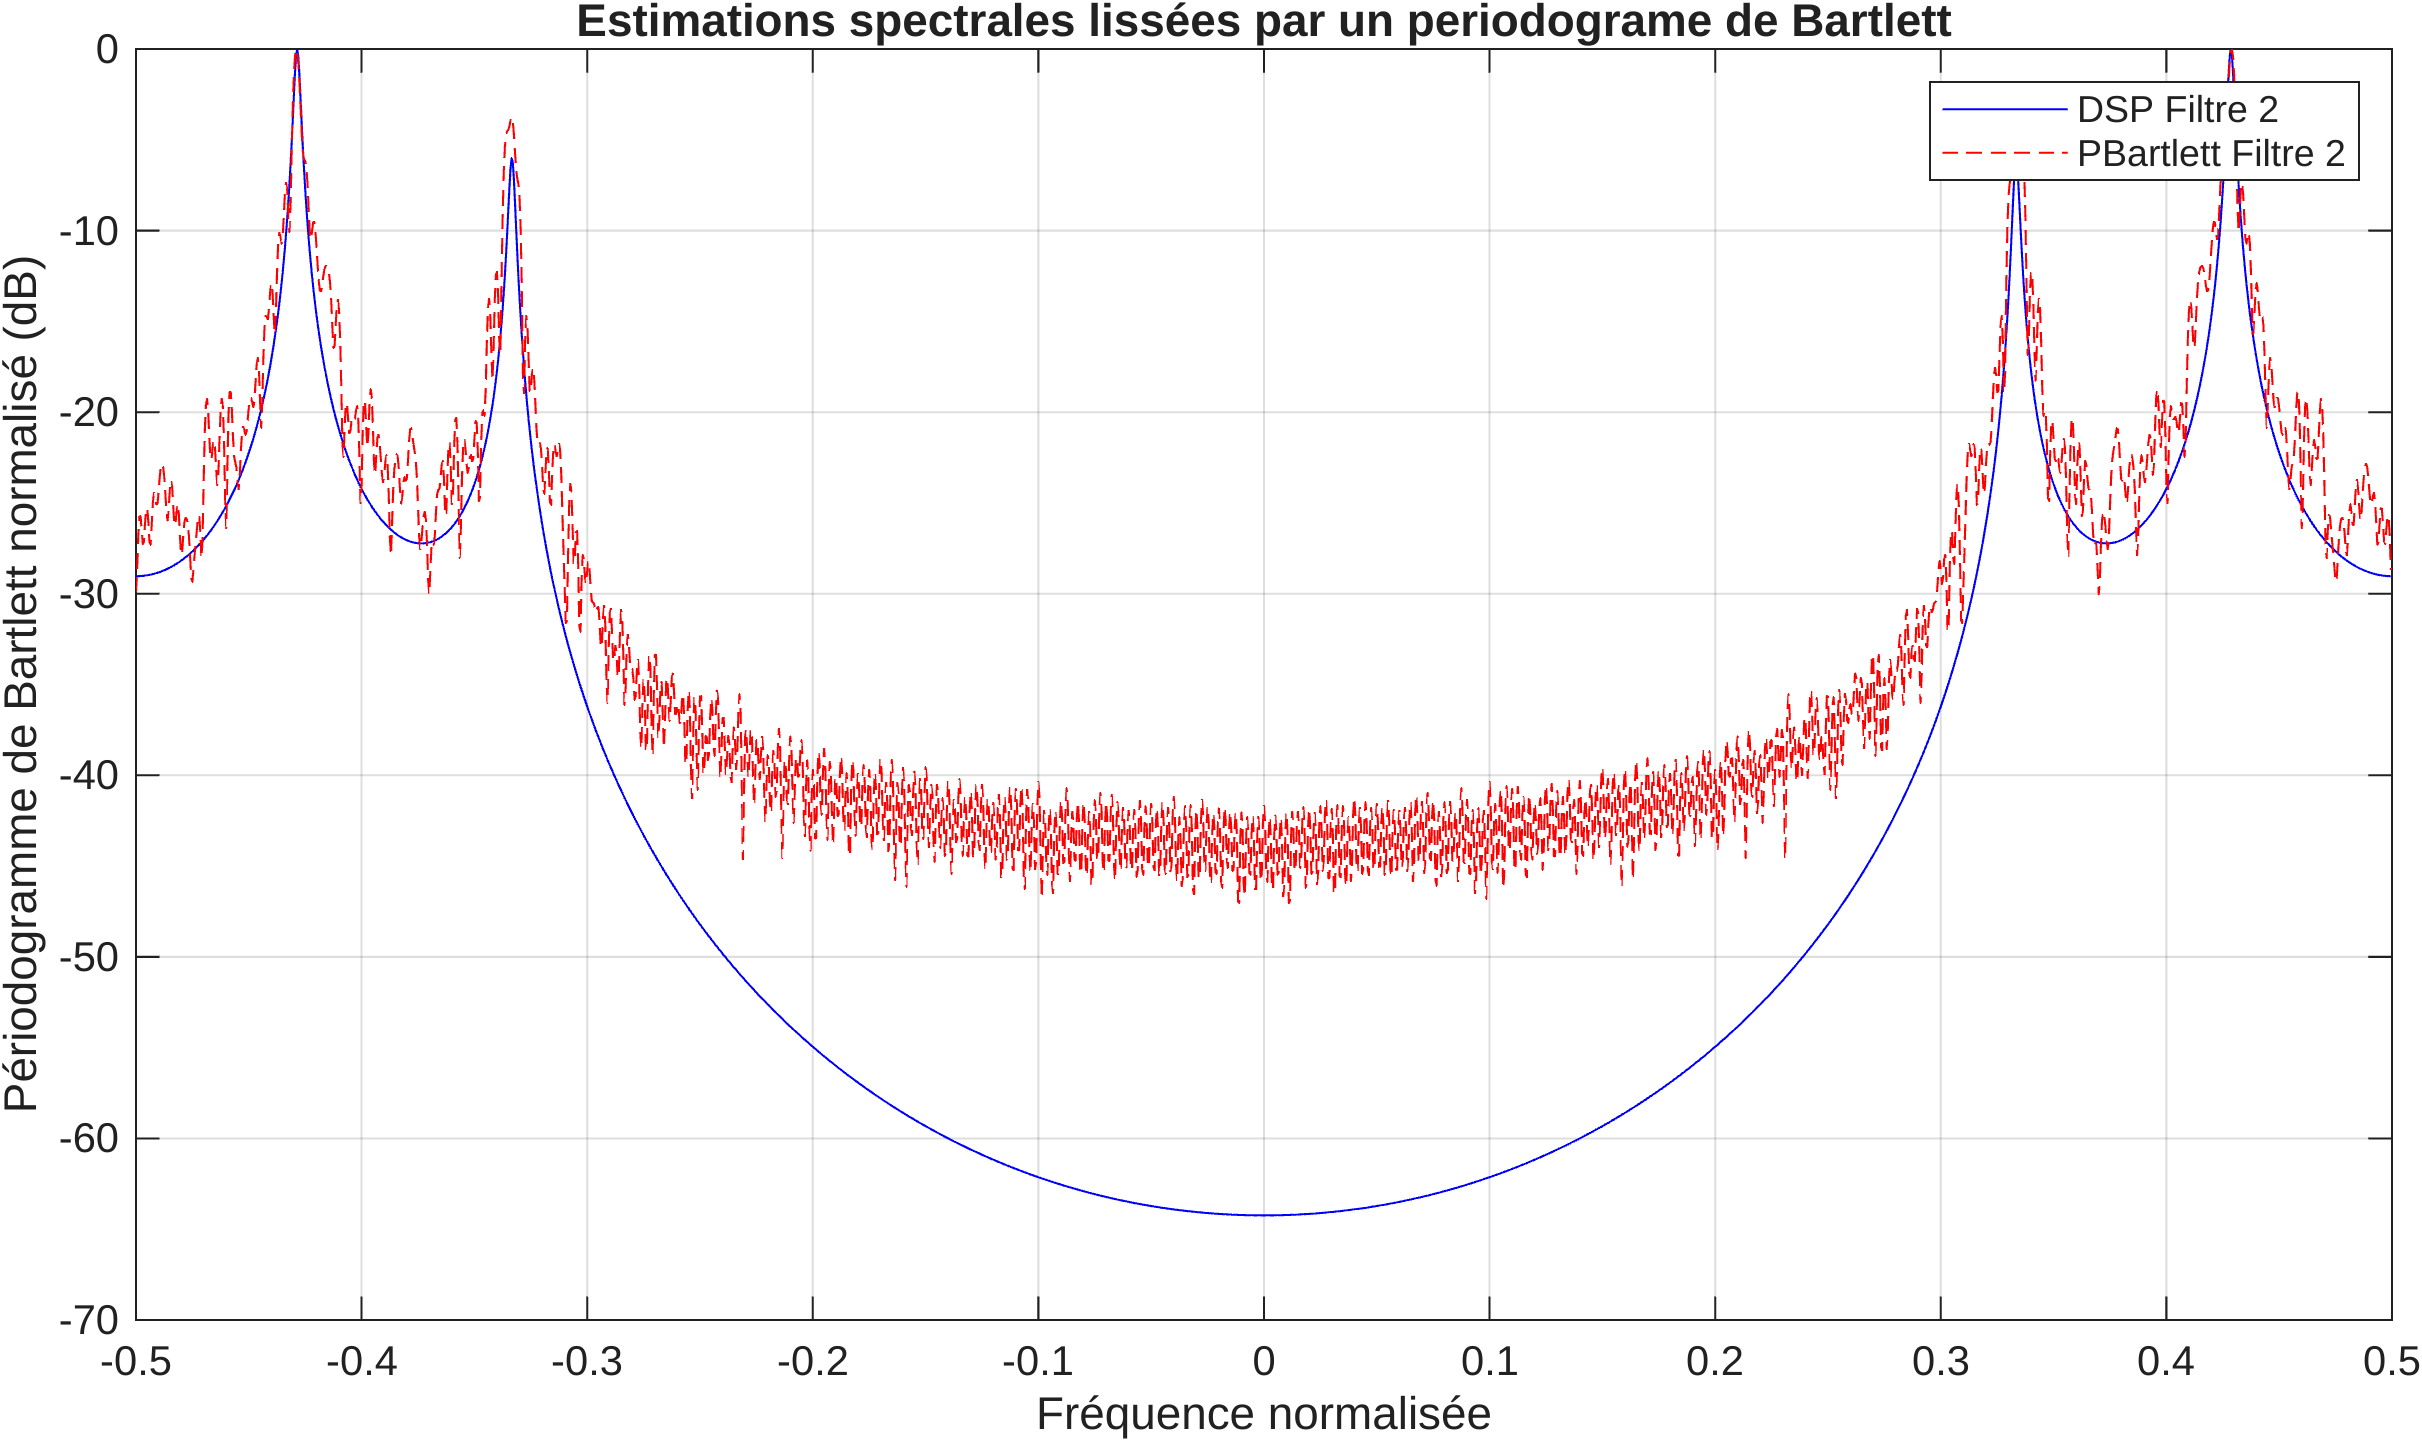
\includegraphics[width=\linewidth]{fig10.png}
    \caption{Processus AR ($M_{\text{AR}} = 400$, $K = 5$)}
    \label{fig:bartlett_ar}
  \end{subfigure}
  \caption{Périodogrammes de Bartlett pour les processus MA et AR.}
  \label{fig:bartlett}
\end{figure}

\indent On remarque qu'on retrouve des facteurs similaires pour les deux processus (figure~\ref{fig:bartlett}), mais surtout que le périodogramme de Bartlett se heurte au même problème que celui de Daniell, c'est-à-dire que pour le processus à variations spectrales rapides (figure~\ref{fig:bartlett_ar}), l'estimateur ne réduit la variance que d'un facteur 5, ce qui laisse le tracé fortement perturbé par le bruit.

De plus, le périodogramme de Bartlett entraîne deux problèmes supplémentaires :
\\- Une fuite spectrale, clairement observable sur le tracé du processus AR (figure~\ref{fig:bartlett_ar}), due au fenêtrage temporel par des portes, donc des convolutions fréquentielles par des sinus cardinaux.
\\- Une perte d'information aux extrémités de chacun des blocs causé par son découpage en $K$ blocs disjoints.
\newline
Périodogramme de Welch :\\
\indent Welch reprend le principe du périodogramme de Bartlett mais cherche à résoudre les deux problèmes cités ci-dessus. Premièrement, en fenêtrant par une fenêtre non rectangulaire, par exemple une fenêtre de Hann. Puis en considérant un taux de recouvrement entre les différentes fenêtres.

\begin{equation}
  I_i(f) = \frac{1}{M \cdot U} \left| \sum_{n=0}^{M-1} x_i(n) w(n) e^{-j 2 \pi f n} \right|^2
\end{equation}
  où $U$ est le facteur de normalisation de la puissance de la fenêtre :
\begin{equation}
  U = \frac{1}{M} \sum_{n=0}^{M-1} |w(n)|^2
\end{equation}
  L'estimateur de Welch est la moyenne de ces $K$ spectres :
\begin{equation}
  \hat{S}_{\text{Welch}}(f) = \frac{1}{K} \sum_{i=1}^{K} I_i(f)
\end{equation}
Pour optimiser le choix de la taille des fenêtres dans le cas de l'estimateur de Welch il faut prendre en compte la géométrie de la fenêtre considérée. Pour une fenêtre de Hann, la largeur de son lobe principal est 1,5 à 2 fois plus large que celui d'une fenêtre rectangulaire. Ainsi on a :

\begin{equation}
    \Delta f \approx \frac{1{,}5}{M}
\end{equation}
\begin{equation}
    \Delta f < \Delta_{FWHM} \iff M > \frac{1{,}5}{\Delta_{FWHM}}
\end{equation}

Dans la suite on considère un recouvrement de 50\,\%, ainsi le nombre $K$ de blocs est quasiment doublé par rapport à l'estimateur Bartlett.

\begin{equation}
    K_{Welch} \approx \frac{2N}{M} - 1 \approx 2K_{Bartlett}
    \label{K Welch}
\end{equation}

Application numérique :
$$
    M_{MA} > 90 \implies M_{MA} = 100
$$
$$
    M_{AR} > 469 \implies M_{AR} = 470
$$

\begin{figure}[htbp]
  \centering
  \begin{subfigure}{0.49\linewidth}
    \centering
    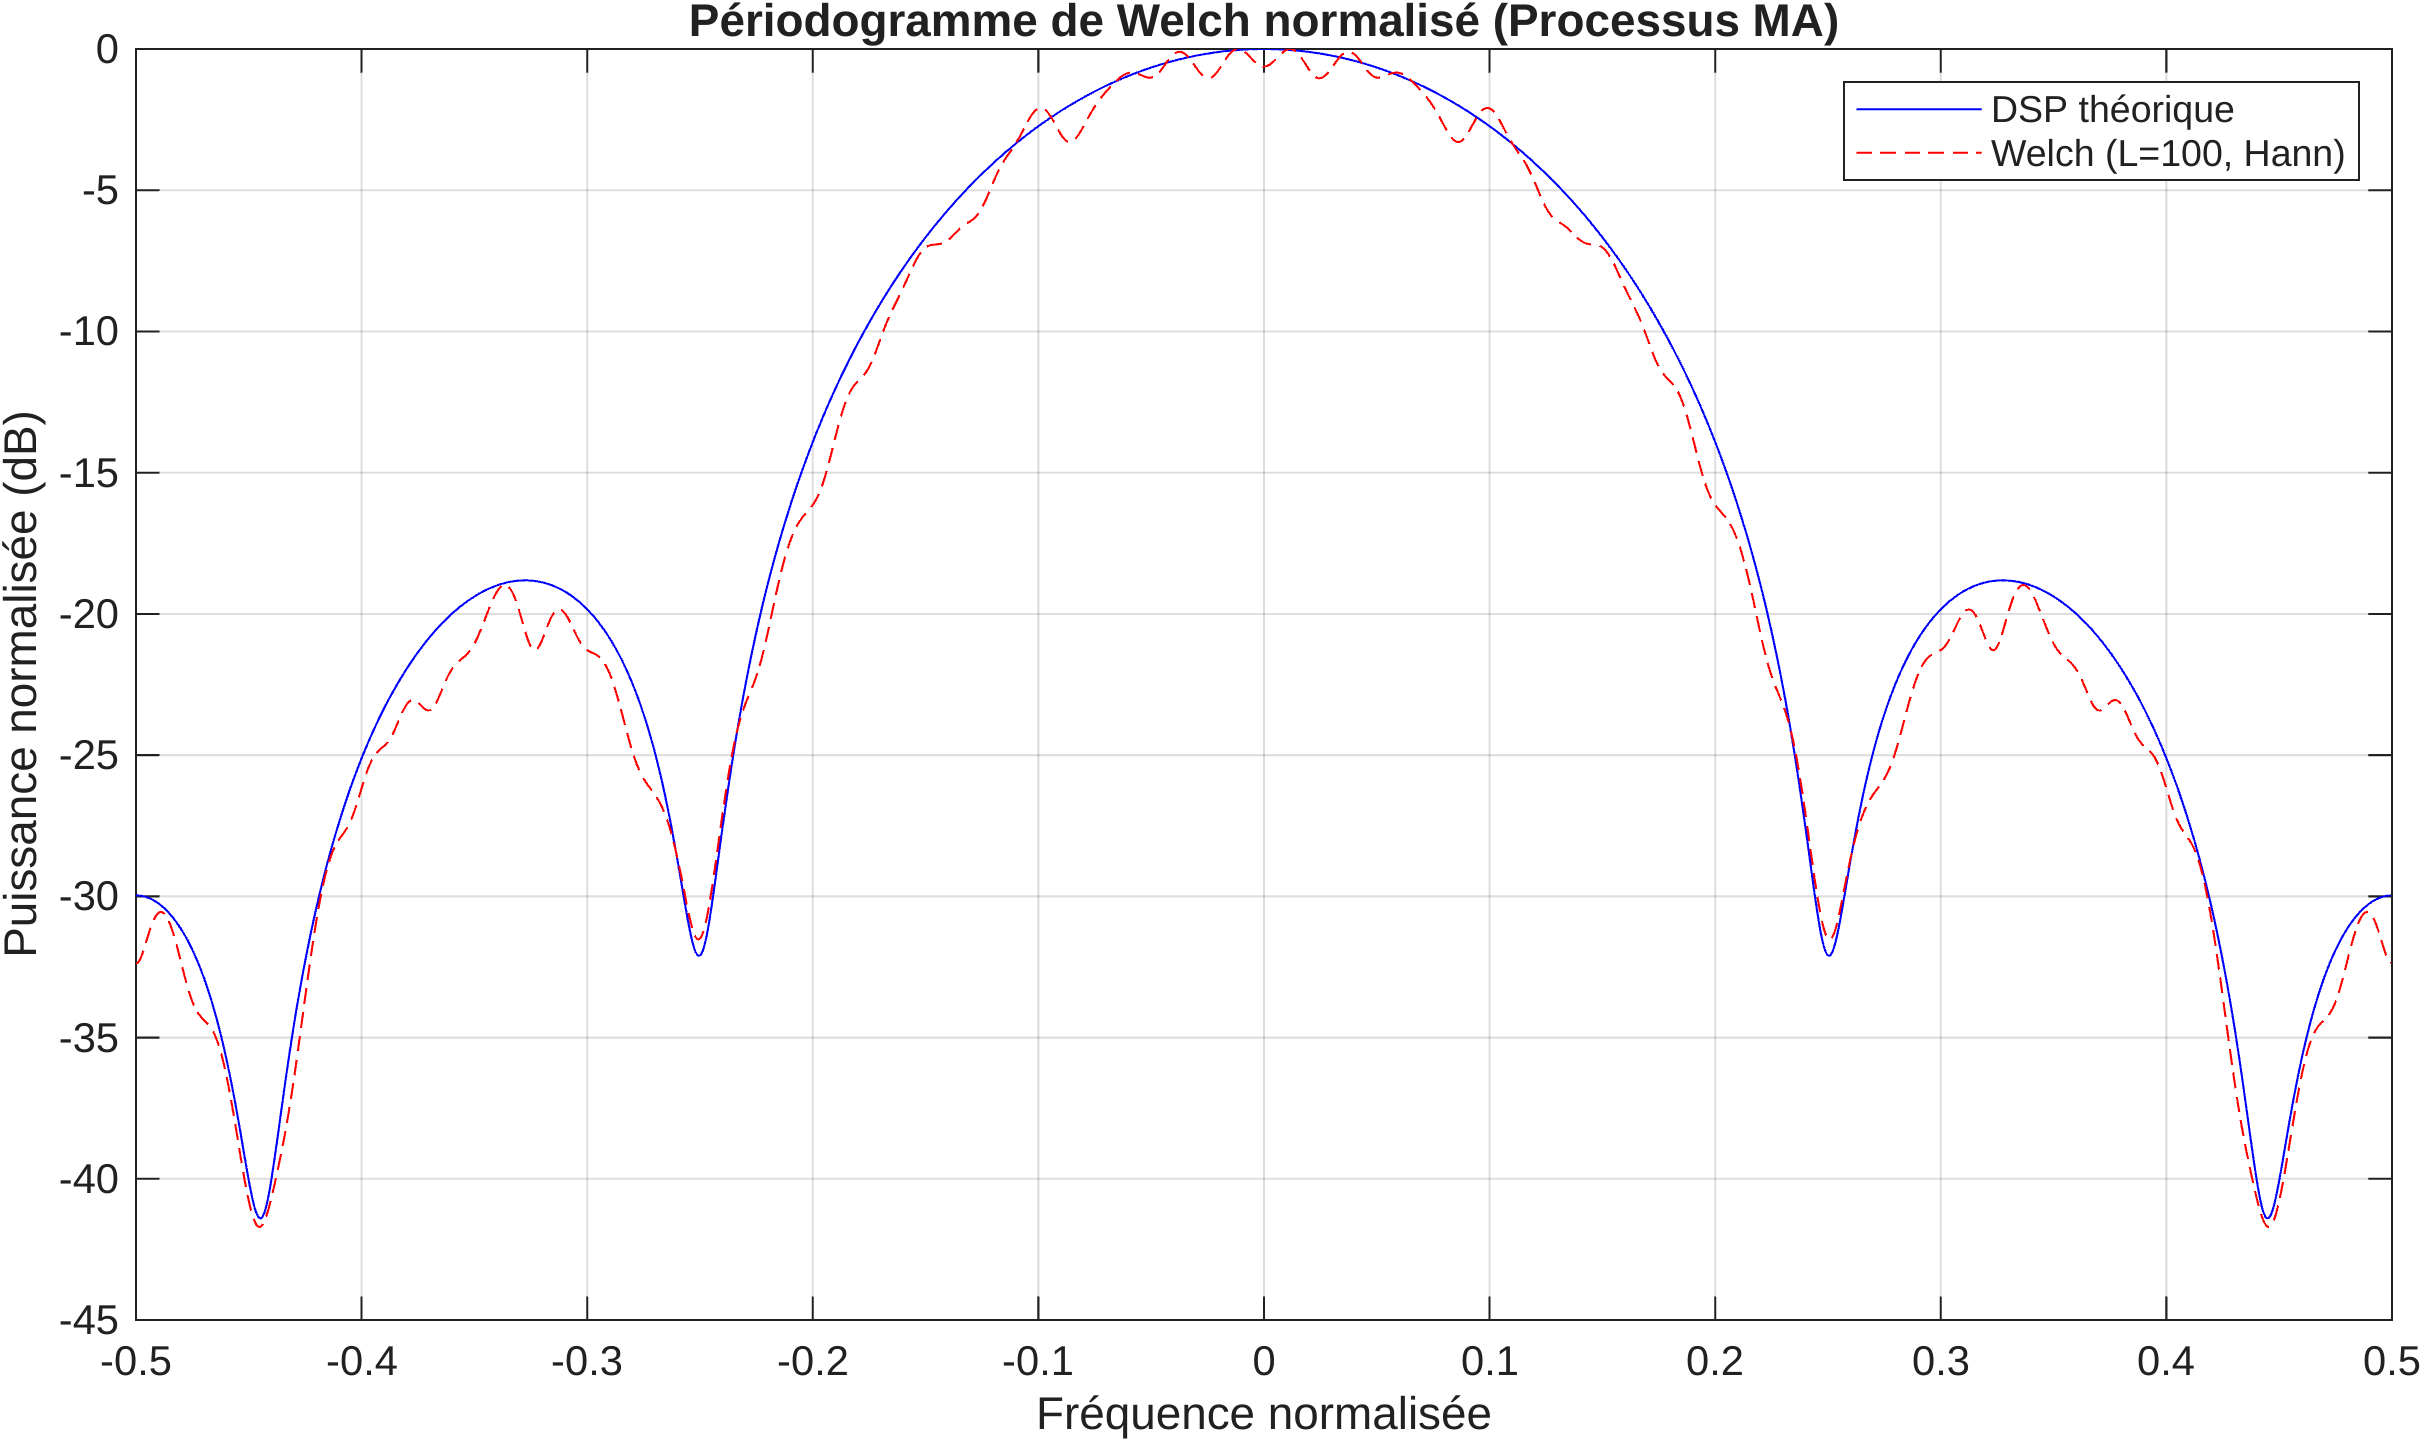
\includegraphics[width=\linewidth]{fig11.png}
    \caption{Processus MA ($M = 100$)}
    \label{fig:welch_ma}
  \end{subfigure}
  \hfill
  \begin{subfigure}{0.49\linewidth}
    \centering
    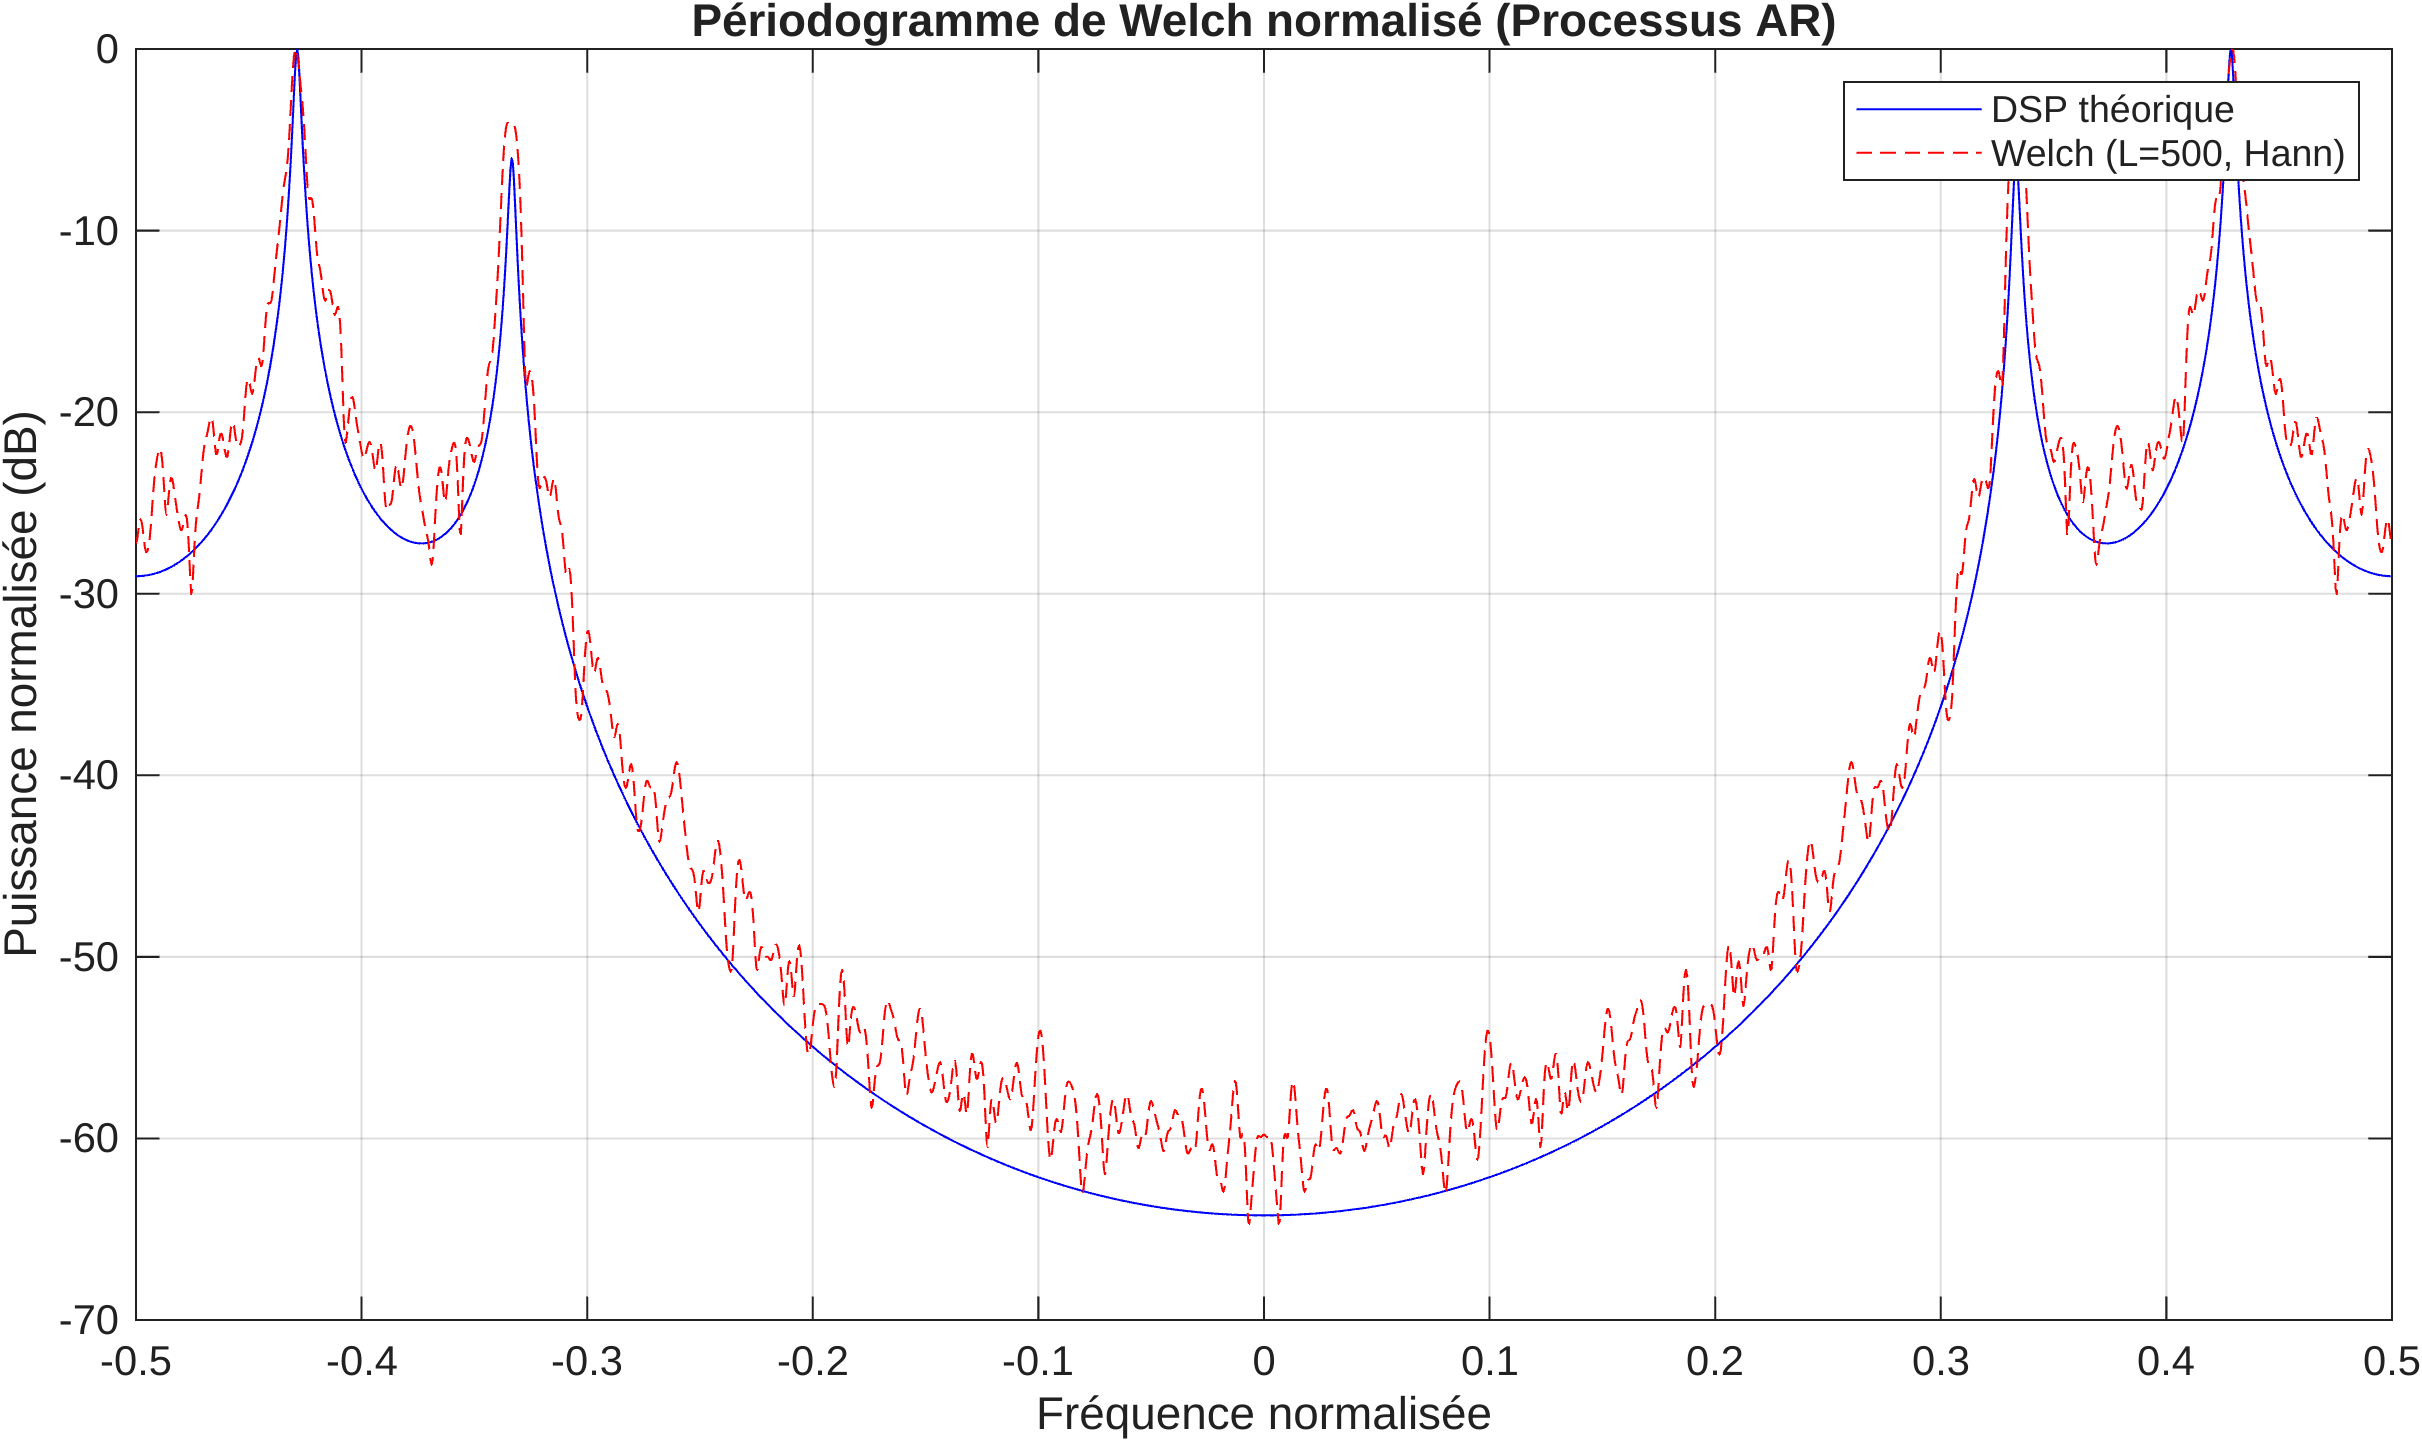
\includegraphics[width=\linewidth]{fig12.png}
    \caption{Processus AR ($M = 470$)}
    \label{fig:welch_ar}
  \end{subfigure}
  \caption{Périodogrammes de Welch pour les processus MA et AR (recouvrement de 50\,\%).}
  \label{fig:welch}
\end{figure}

Donc pour cet estimateur selon \eqref{K Welch} on a :
\begin{equation}
    \operatorname{Var}(\hat{S}_{\text{Welch}}) \approx \frac{1}{2K_{Bartlett}} S_x^2
\end{equation}

Visiblement, l'estimateur de Welch (figure~\ref{fig:welch}) corrige bien les problèmes du périodogramme de Bartlett causés par le fenêtrage rectangulaire. On remarque clairement la réduction des effets de bords qui sur le tracé ne provoquent pas de remontées artificielles. De plus, pour le processus MA (figure~\ref{fig:welch_ma}) la variance est réduite d'un facteur 50 tandis que pour le processus AR (figure~\ref{fig:welch_ar}) d'un facteur 10 ce qui reste bien mieux que le facteur 5 commun aux estimateurs de Daniell et de Bartlett.

Ainsi Welch combine le meilleur des deux estimateurs :
\\- Il évite les remontées artificielles de plancher de bruit (fuites de Bartlett) grâce au fenêtrage de Hann,
\\- Il compense la perte de résolution par le recouvrement qui maximise le nombre de sous-blocs moyennés $K$.

\bigskip
Corrélogramme (Blackman-Tukey) :\\
\indent Contrairement aux approches précédentes qui opèrent directement sur le périodogramme standard dans le domaine spectral, la méthode du corrélogramme (estimateur de Blackman-Tukey) repose sur le théorème de Wiener-Khintchine. Elle consiste à estimer d'abord la fonction d'autocorrélation du signal, puis à en calculer la transformée de Fourier après fenêtrage temporel.

L'autocorrélation est estimée par l'estimateur biaisé :
\begin{equation}
    \hat{r}_x(k) = \frac{1}{N} \sum_{n=0}^{N-1-|k|} x(n+|k|) x(n), \qquad |k| \leq K_{\max}
\end{equation}
Pour les retards $k$ élevés, l'estimation devient fortement bruitée car calculée sur peu d'échantillons. On tronque donc la séquence à un retard maximal $K_{\max} \ll N$ et on applique une fenêtre de pondération symétrique $w(k)$ :
\begin{equation}
    \hat{S}_{\text{BT}}(f) = \sum_{k=-K_{\max}}^{K_{\max}} w(k)\, \hat{r}_x(k)\, e^{-j 2 \pi f k}
\end{equation}
Dans le code Matlab, on choisit une fenêtre triangulaire (Bartlett) de taille $2 K_{\max} + 1$ avec $K_{\max} = 100$. L'intérêt de ce choix est qu'il garantit un spectre strictement positif ($\hat{S}_{\text{BT}}(f) \geq 0$) pour toute fréquence, la transformée de Fourier d'un triangle étant un sinus cardinal au carré.

La condition de non-distorsion spectrale impose une résolution fréquentielle suffisante :
\begin{equation}
    \Delta f \approx \frac{1}{K_{\max}} < \Delta_{FWHM} \iff K_{\max} > \frac{1}{\Delta_{FWHM}}
\end{equation}

Application numérique :
$$K_{MA} > 60 \implies K_{MA, choisi} = 100$$
$$K_{AR} > 313 \implies K_{AR} = 100 \text{ (valeur retenue dans le code)}$$

Dans le cas du corrélogramme avec fenêtre triangulaire, on a :
\begin{equation}
    \operatorname{Var}(\hat{S}_{\text{BT}}) \approx \frac{2}{3} \frac{K_{\max}}{N} S_x^2
\end{equation}

Ainsi, avec $K_{\max} = 100$ et $N = 2000$, la variance est réduite d'un facteur 30 par rapport au périodogramme standard.

\begin{figure}[htbp]
  \centering
  \begin{subfigure}{0.49\linewidth}
    \centering
    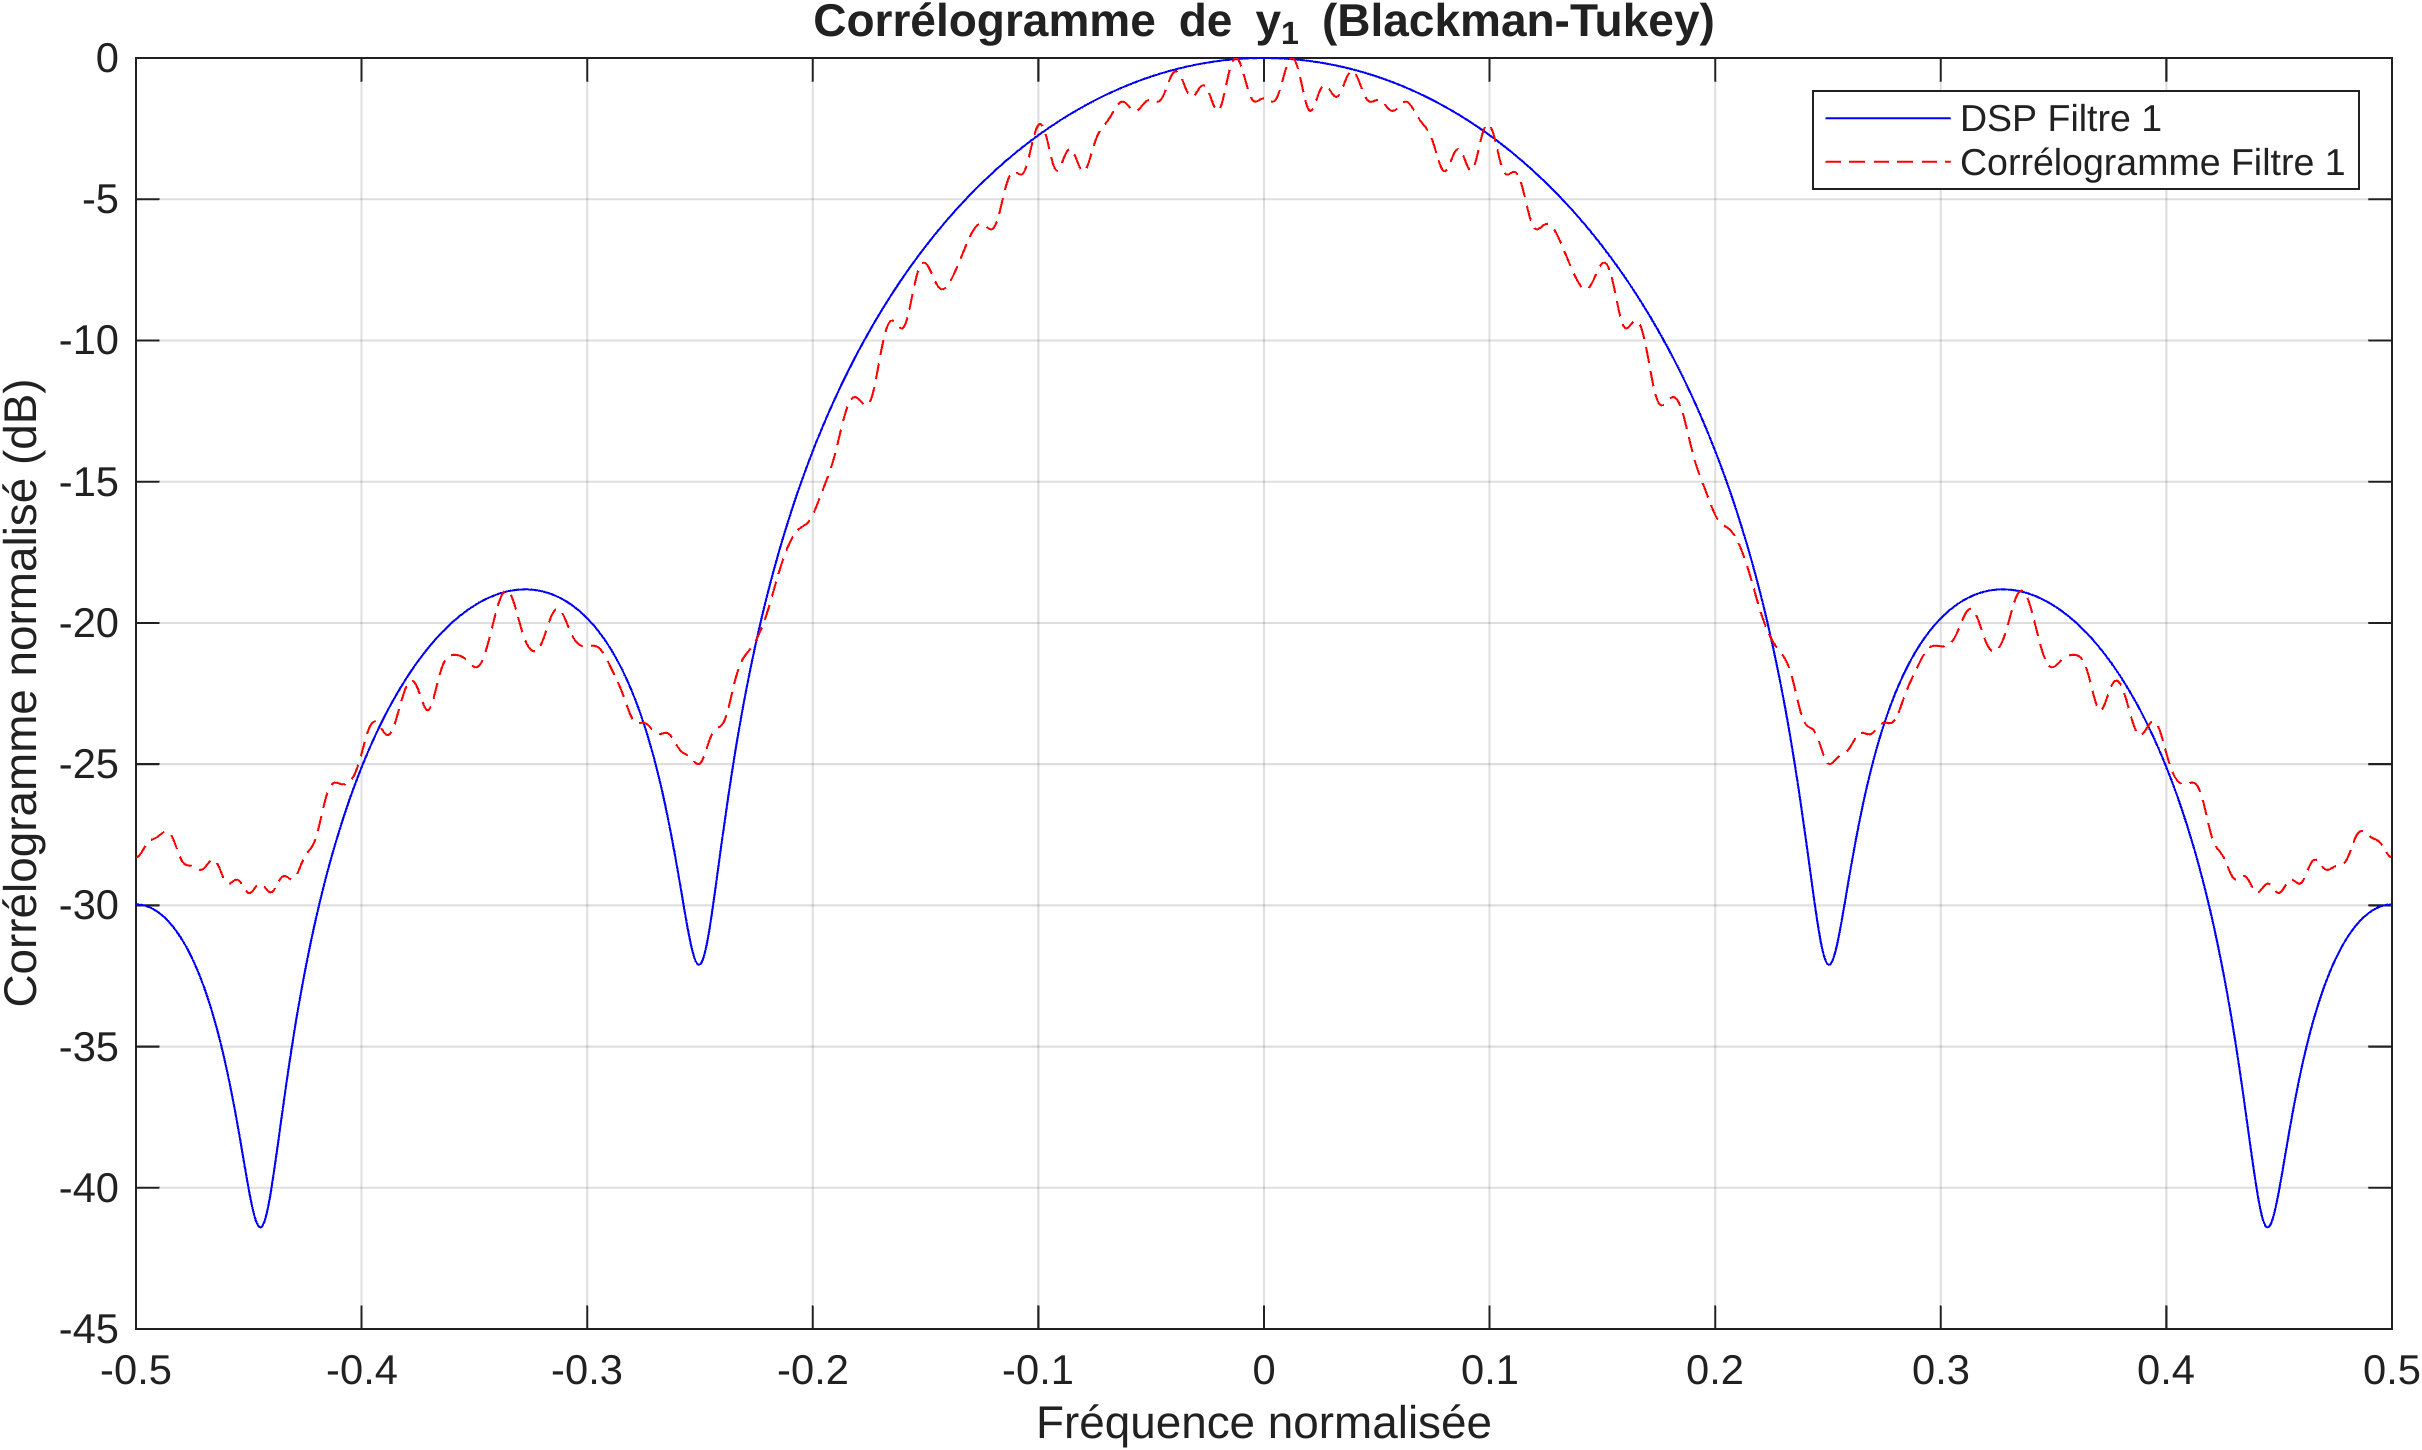
\includegraphics[width=\linewidth]{fig13.png}
    \caption{Processus MA ($K_{\max} = 100$)}
    \label{fig:correlogramme_ma}
  \end{subfigure}
  \hfill
  \begin{subfigure}{0.49\linewidth}
    \centering
    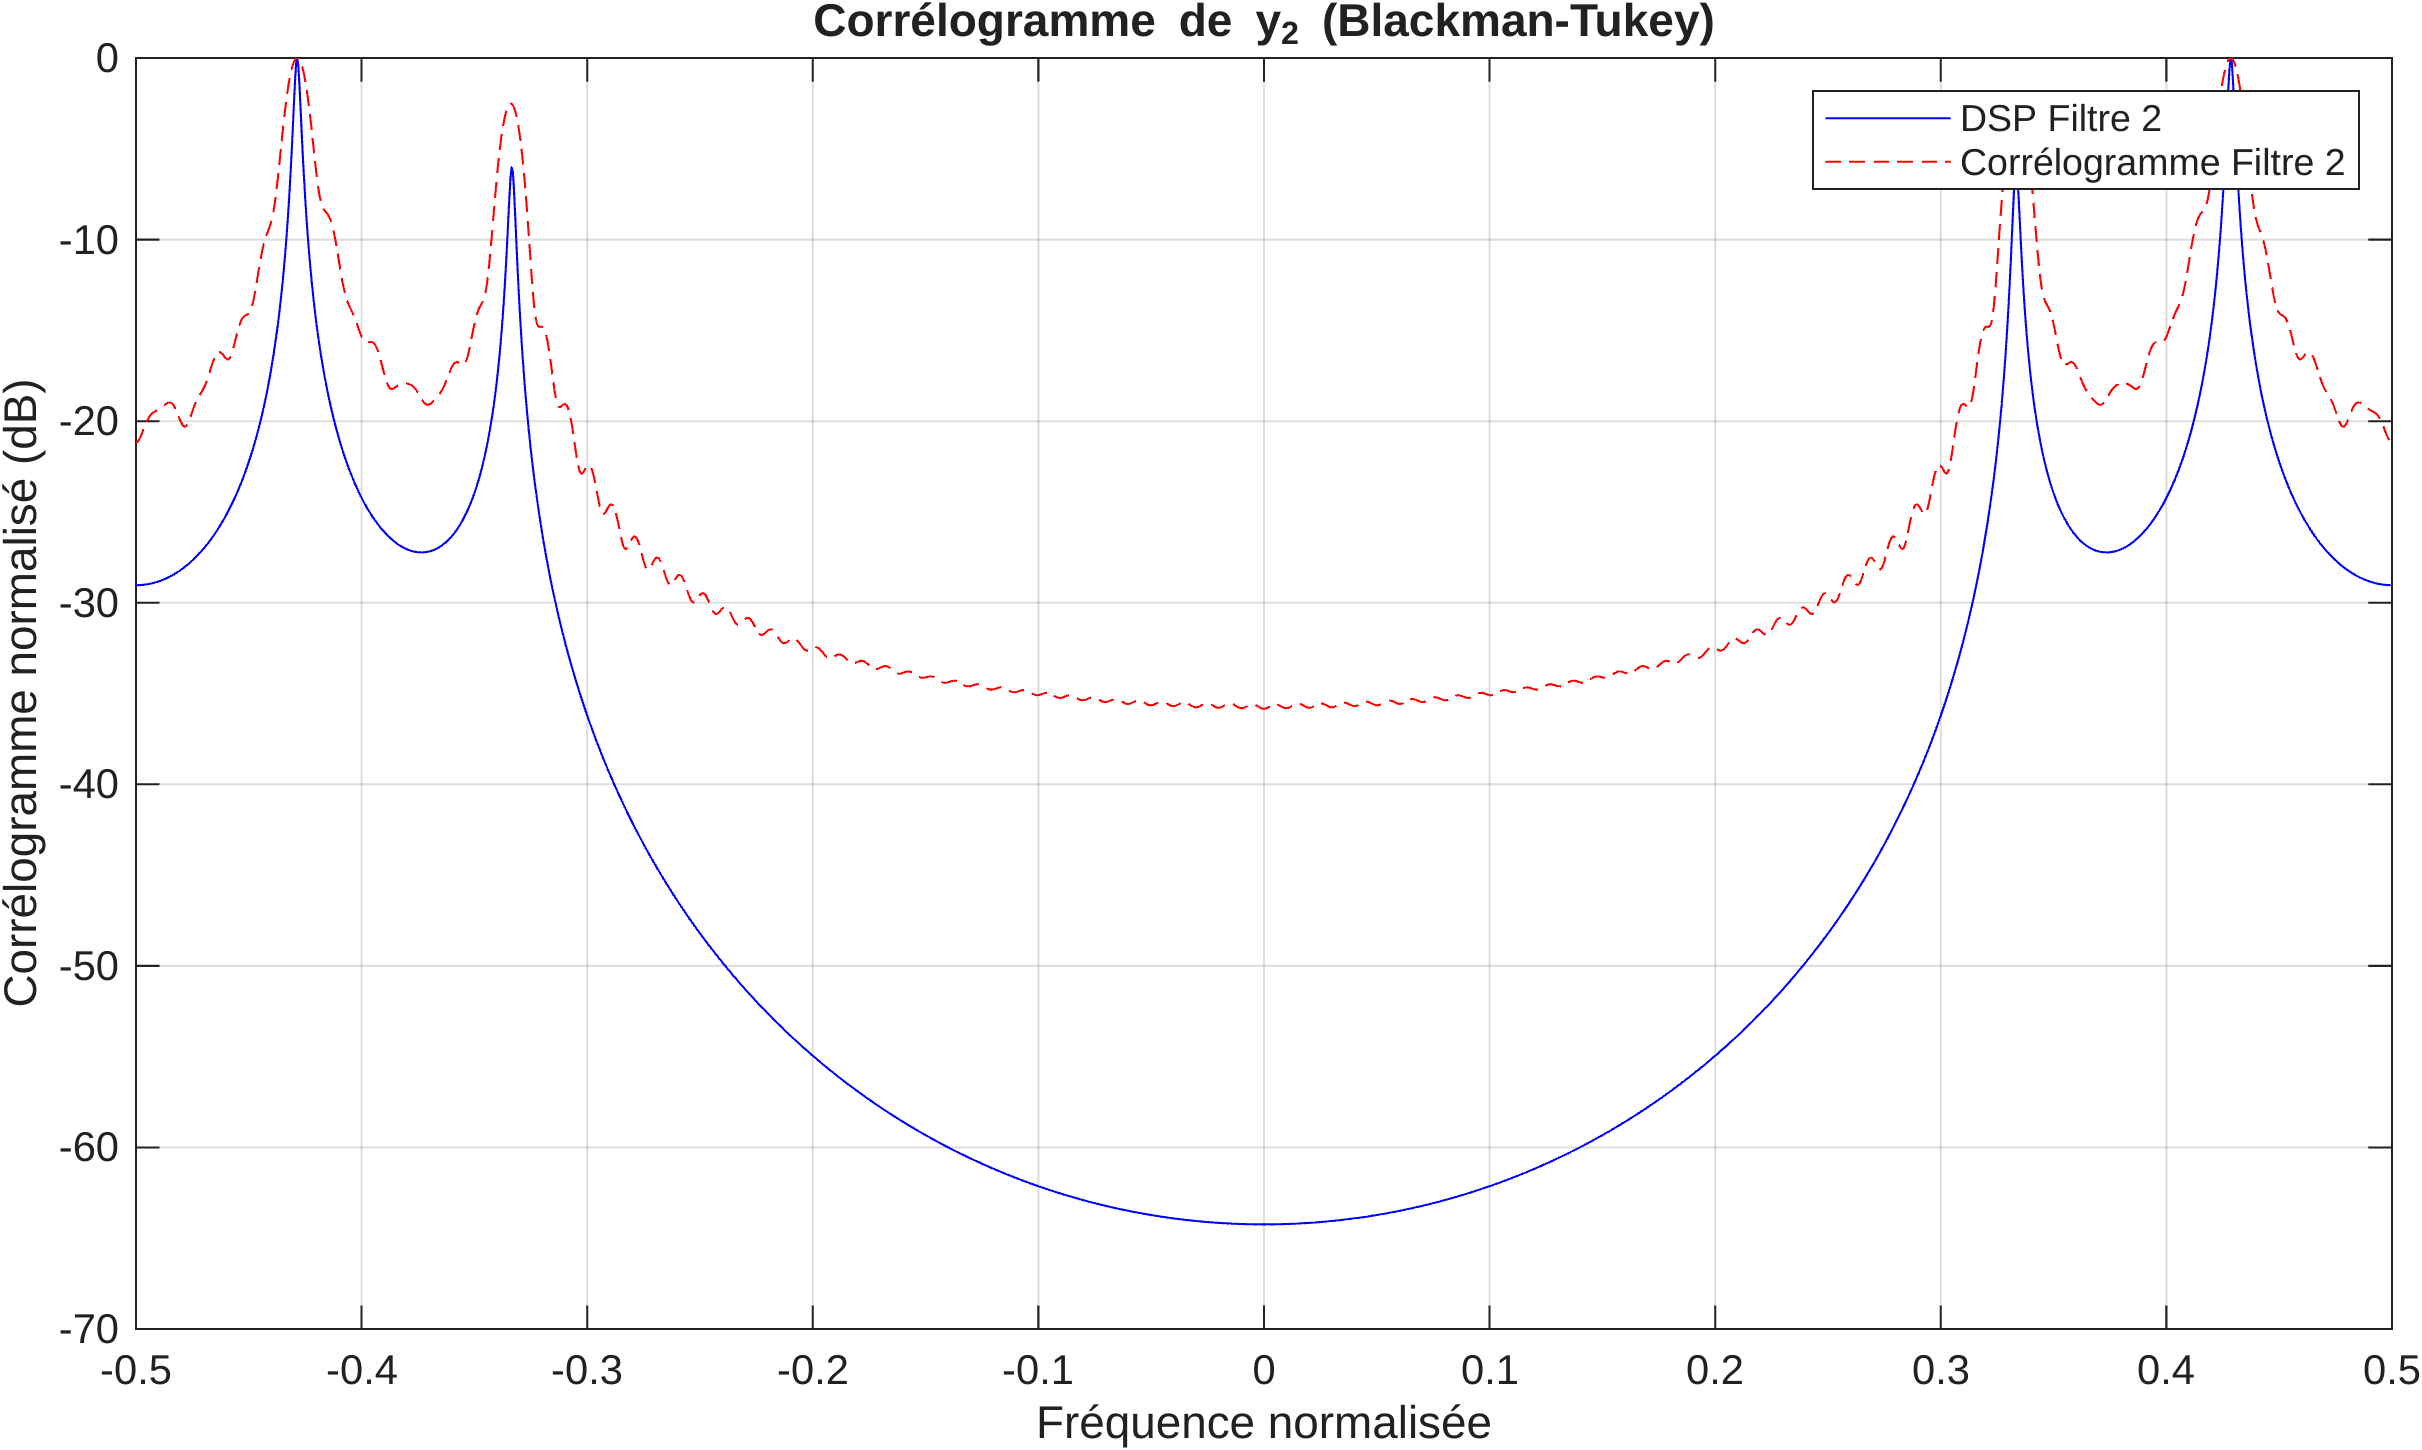
\includegraphics[width=\linewidth]{fig14.png}
    \caption{Processus AR ($K_{\max} = 100$)}
    \label{fig:correlogramme_ar}
  \end{subfigure}
  \caption{Corrélogrammes de Blackman-Tukey pour les processus MA et AR (fenêtre triangulaire).}
  \label{fig:correlogramme}
\end{figure}

\indent On remarque que sur la figure~\ref{fig:correlogramme} :
\\- Pour le processus MA (figure~\ref{fig:correlogramme_ma}), l'autocorrélation s'annule théoriquement au-delà de 4 retards. La valeur $K_{\max} = 100$ vérifie largement la condition de non-distorsion ($K_{MA} > 60$) : l'estimateur restitue parfaitement les creux en $\pm 1/4$ et $\pm 4/9$ tout en divisant la variance par 30.
\\- Pour le processus AR (figure~\ref{fig:correlogramme_ar}), la condition de non-distorsion nécessiterait $K_{max} > 313$ du fait des variations spectrales très rapides ($\Delta_{FWHM} \approx 0{,}0032$). Avec $K_{\max} = 100$, la résolution est limitée ($\Delta f = 0{,}01$), ce qui élargit et atténue légèrement les pics de résonance, mais le lissage est très net et supprime les fluctuations du périodogramme brut.


\subsection{Méthode à mettre en œuvre}

\subsubsection{Étape n°1 : centrage et intégration}

Dans cette partie, on reprend les notations du sujet : le signal étudié $x(n)$ contient
$M$ échantillons, et $N$ désigne désormais la taille des blocs utilisée à l'étape 2.

Le signal $x(n)$ est d'abord centré en lui retirant sa moyenne empirique :
\begin{equation}
  x_c(n) = x(n) - \bar{x}, \qquad \bar{x} = \frac{1}{M}\sum_{k=1}^{M} x(k).
  \label{eq:centrage}
\end{equation}
Il est ensuite intégré, c'est-à-dire que l'on fait la somme cumulée des échantillons centrés :
\begin{equation}
  y(n) = \sum_{k=1}^{n} x_c(k)
  \quad \iff \quad
  y(n) = y(n-1) + x_c(n), \quad y(0) = 0.
  \label{eq:integration}
\end{equation}
C'est la forme récursive de \eqref{eq:integration} qui est utilisée dans le code Matlab.

L'intégration peut être vue comme un filtrage de $x_c(n)$ par le filtre de fonction de transfert :
\begin{equation}
  H_{int}(z) = \frac{1}{1 - z^{-1}},
  \qquad
  \left|H_{int}(\nu)\right| = \frac{1}{2\left|\sin(\pi\nu)\right|}.
  \label{eq:Hint}
\end{equation}
Ce filtre est un RII dont le pôle $z = 1$ est situé sur le cercle unité : il n'est donc pas
stable au sens EBSB. Son gain tend vers l'infini quand $\nu \to 0$ : l'intégration amplifie
fortement les basses fréquences et atténue les hautes fréquences. Le signal $y(n)$ varie donc
beaucoup plus lentement que $x(n)$.

\subsubsection{Étape n°2 : estimation de la tendance}

On cherche à estimer la tendance $t(n)$ de $y(n)$. Les
figures sont obtenues pour un bruit blanc de $M = 2000$ échantillons et $N = 200$.

\paragraph{2a : régression par blocs}

Le signal est découpé en $L = \lfloor M/N \rfloor$ blocs de $N$ échantillons. Sur chaque
bloc $\mathbf{y}_l$, la tendance est modélisée par un polynôme de degré $d$ : la moyenne
pour $d = 0$, une droite pour $d = 1$, un polynôme pour $d \geq 2$. Sous forme matricielle :
\begin{equation}
  \mathbf{y}_l = \mathbf{A}\boldsymbol{\theta}_l + \mathbf{e}_l,
  \qquad
  \mathbf{A} =
  \begin{pmatrix}
    1 & 1 & \cdots & 1^d \\
    \vdots & \vdots & & \vdots \\
    1 & N & \cdots & N^d
  \end{pmatrix},
\end{equation}
où $\boldsymbol{\theta}_l$ contient les coefficients du polynôme et $\mathbf{e}_l$ l'erreur
de modélisation. On estime $\boldsymbol{\theta}_l$ par les moindres carrés, en minimisant
$\|\mathbf{y}_l - \mathbf{A}\boldsymbol{\theta}\|^2$. En annulant le gradient, on obtient :
\begin{equation}
  \hat{\boldsymbol{\theta}}_l = \left(\mathbf{A}^T\mathbf{A}\right)^{-1}\mathbf{A}^T\mathbf{y}_l .
  \label{eq:mc}
\end{equation}
La tendance globale est ensuite obtenue en concaténant les tendances
$\mathbf{A}\hat{\boldsymbol{\theta}}_l$ des $L$ blocs.

Sur la figure~\ref{fig:tendances}, la tendance est discontinue entre les blocs, puisque
chaque bloc est traité séparément. Plus $d$ est grand, plus le polynôme colle au signal :
il absorbe alors une partie des fluctuations que l'on veut mesurer.

\begin{figure}[htbp]
  \centering
  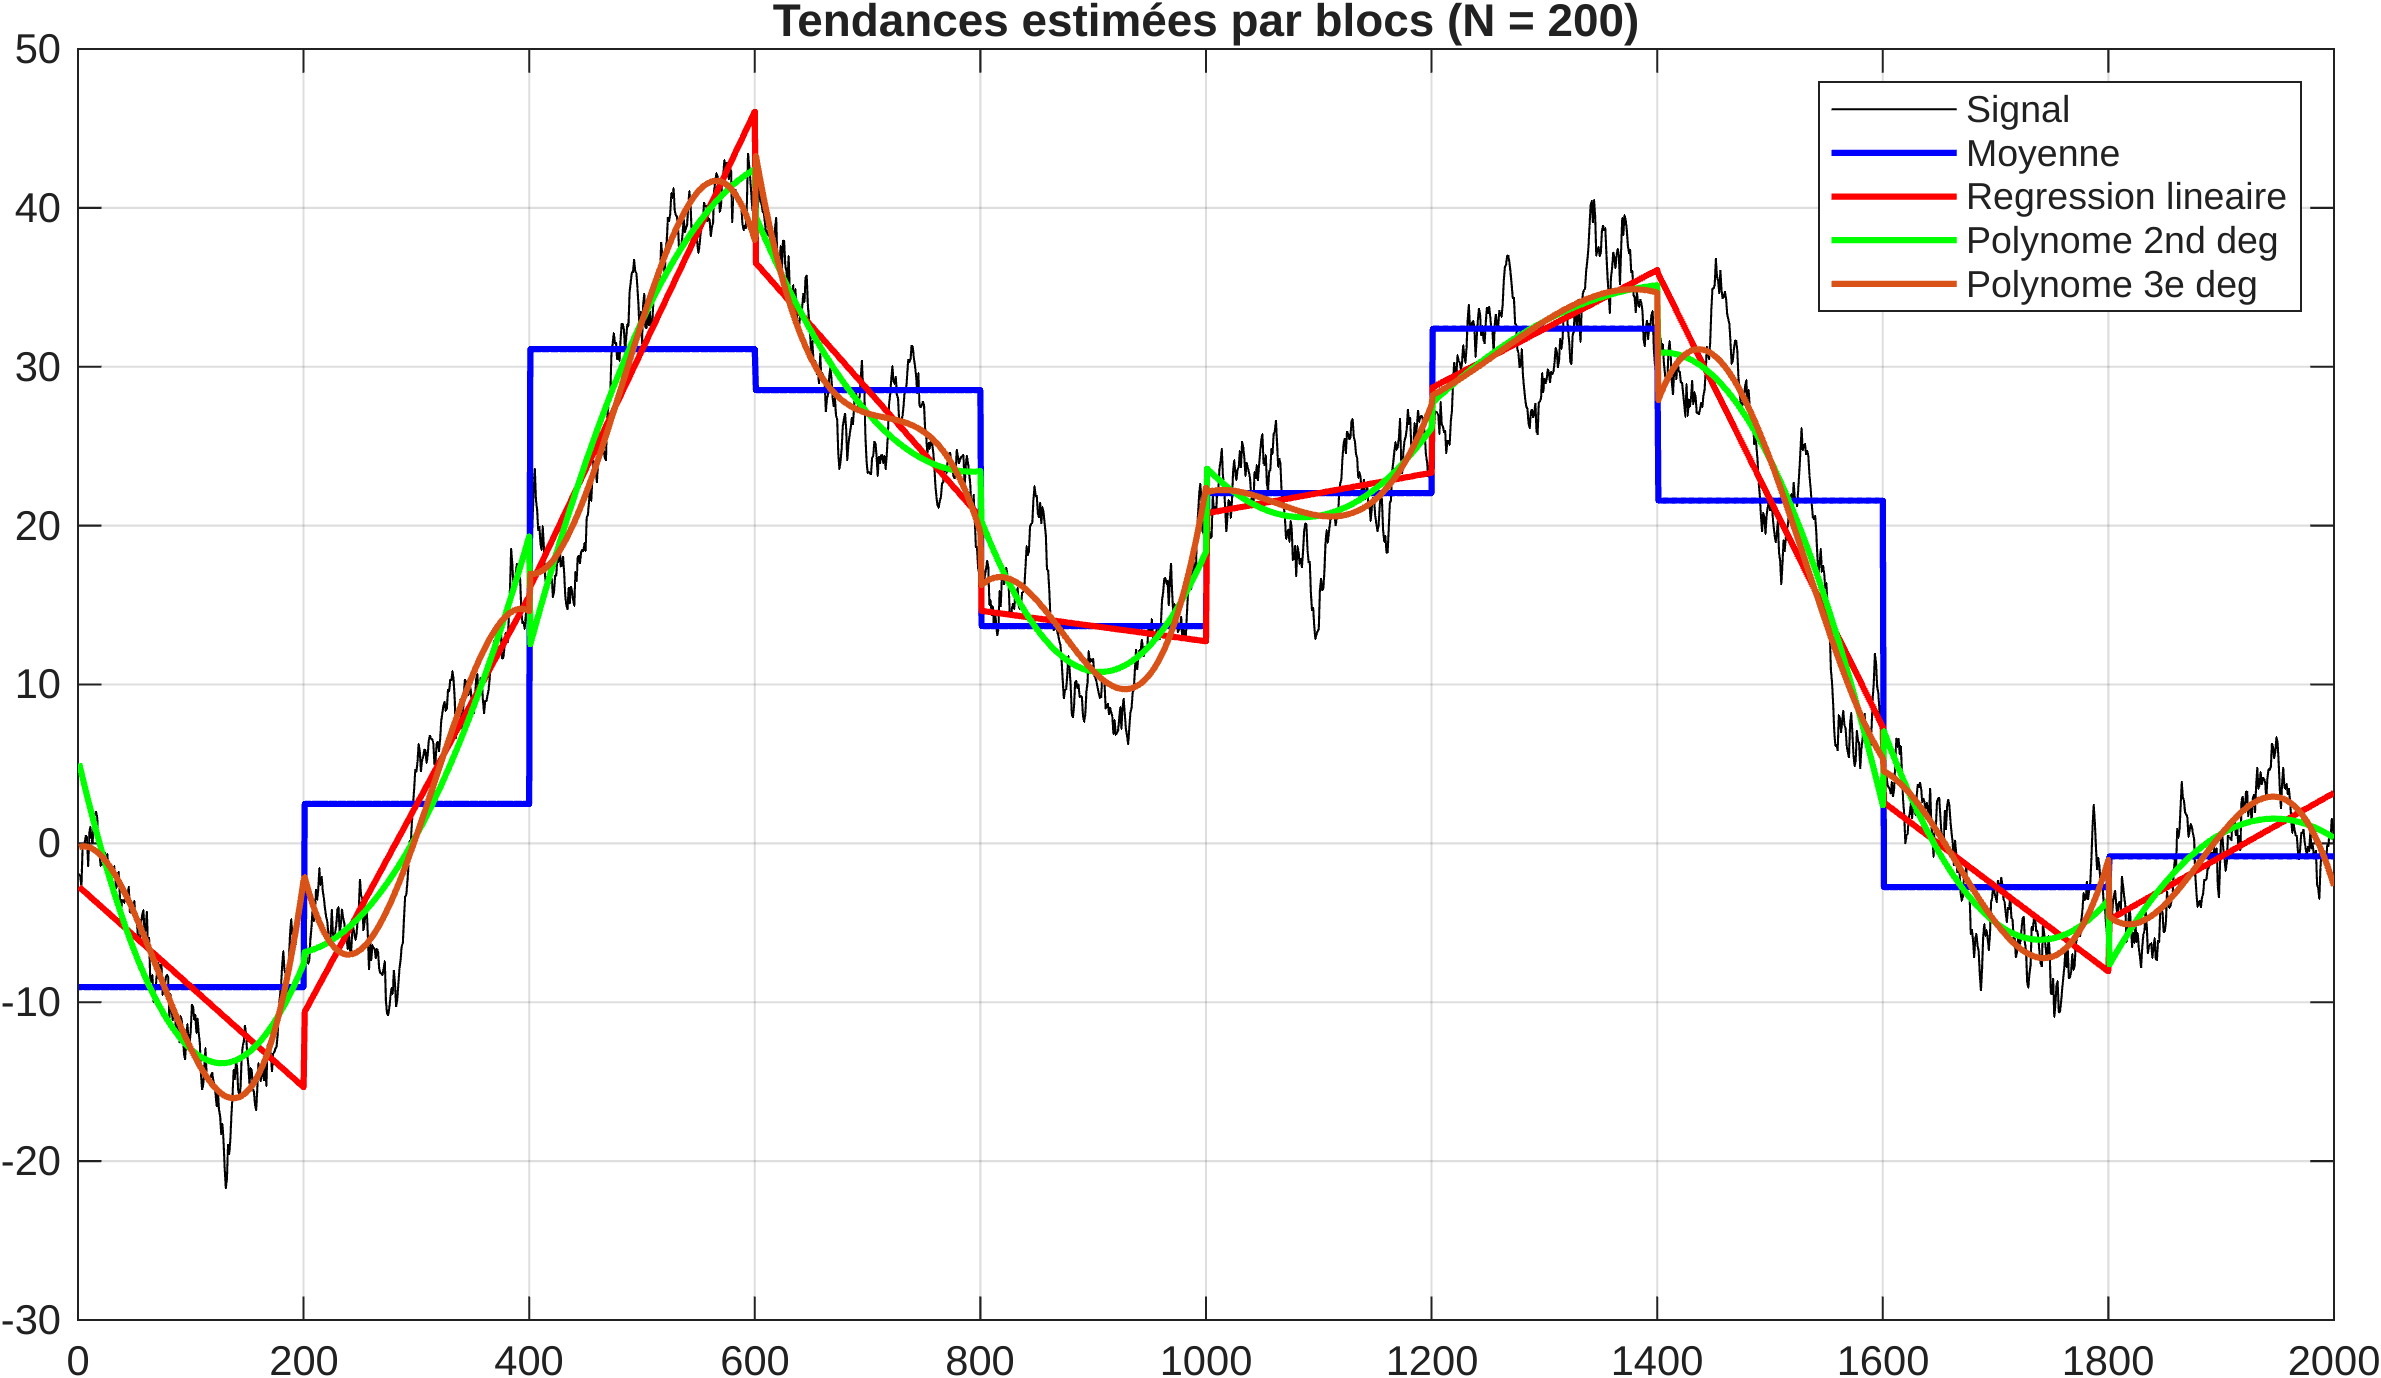
\includegraphics[width=0.7\linewidth]{fig15.png}
  \caption{Tendances estimées par blocs ($N = 200$), pour $d = 0$ à $3$.}
  \label{fig:tendances}
\end{figure}

\paragraph{2b : moyenne glissante}

La tendance est estimée par la moyenne des $N$ derniers échantillons, ce qui revient à
filtrer $y(n)$ :
\begin{equation}
  t(n) = \frac{1}{N}\sum_{k=0}^{N-1} y(n-k),
  \qquad
  H(\nu) = e^{-j\pi\nu(N-1)}\, \frac{\sin(\pi\nu N)}{N\sin(\pi\nu)}.
  \label{eq:H_mg}
\end{equation}
Ce filtre est un passe-bas \textbf{RIF}, \textbf{causal} et \textbf{stable}. Sa réponse
impulsionnelle est symétrique, il est donc à \textbf{phase linéaire} et introduit un
\textbf{retard} de $(N-1)/2$ échantillons. Il n'est \textbf{pas à minimum de phase}, car
ses zéros sont sur le cercle unité.

Ce retard se voit nettement sur la figure~\ref{fig:mg} : la tendance est décalée vers la
droite par rapport au signal. C'est un défaut pour l'étape 3, d'où l'intérêt d'un filtre à
phase nulle.

\begin{figure}[htbp]
  \centering
  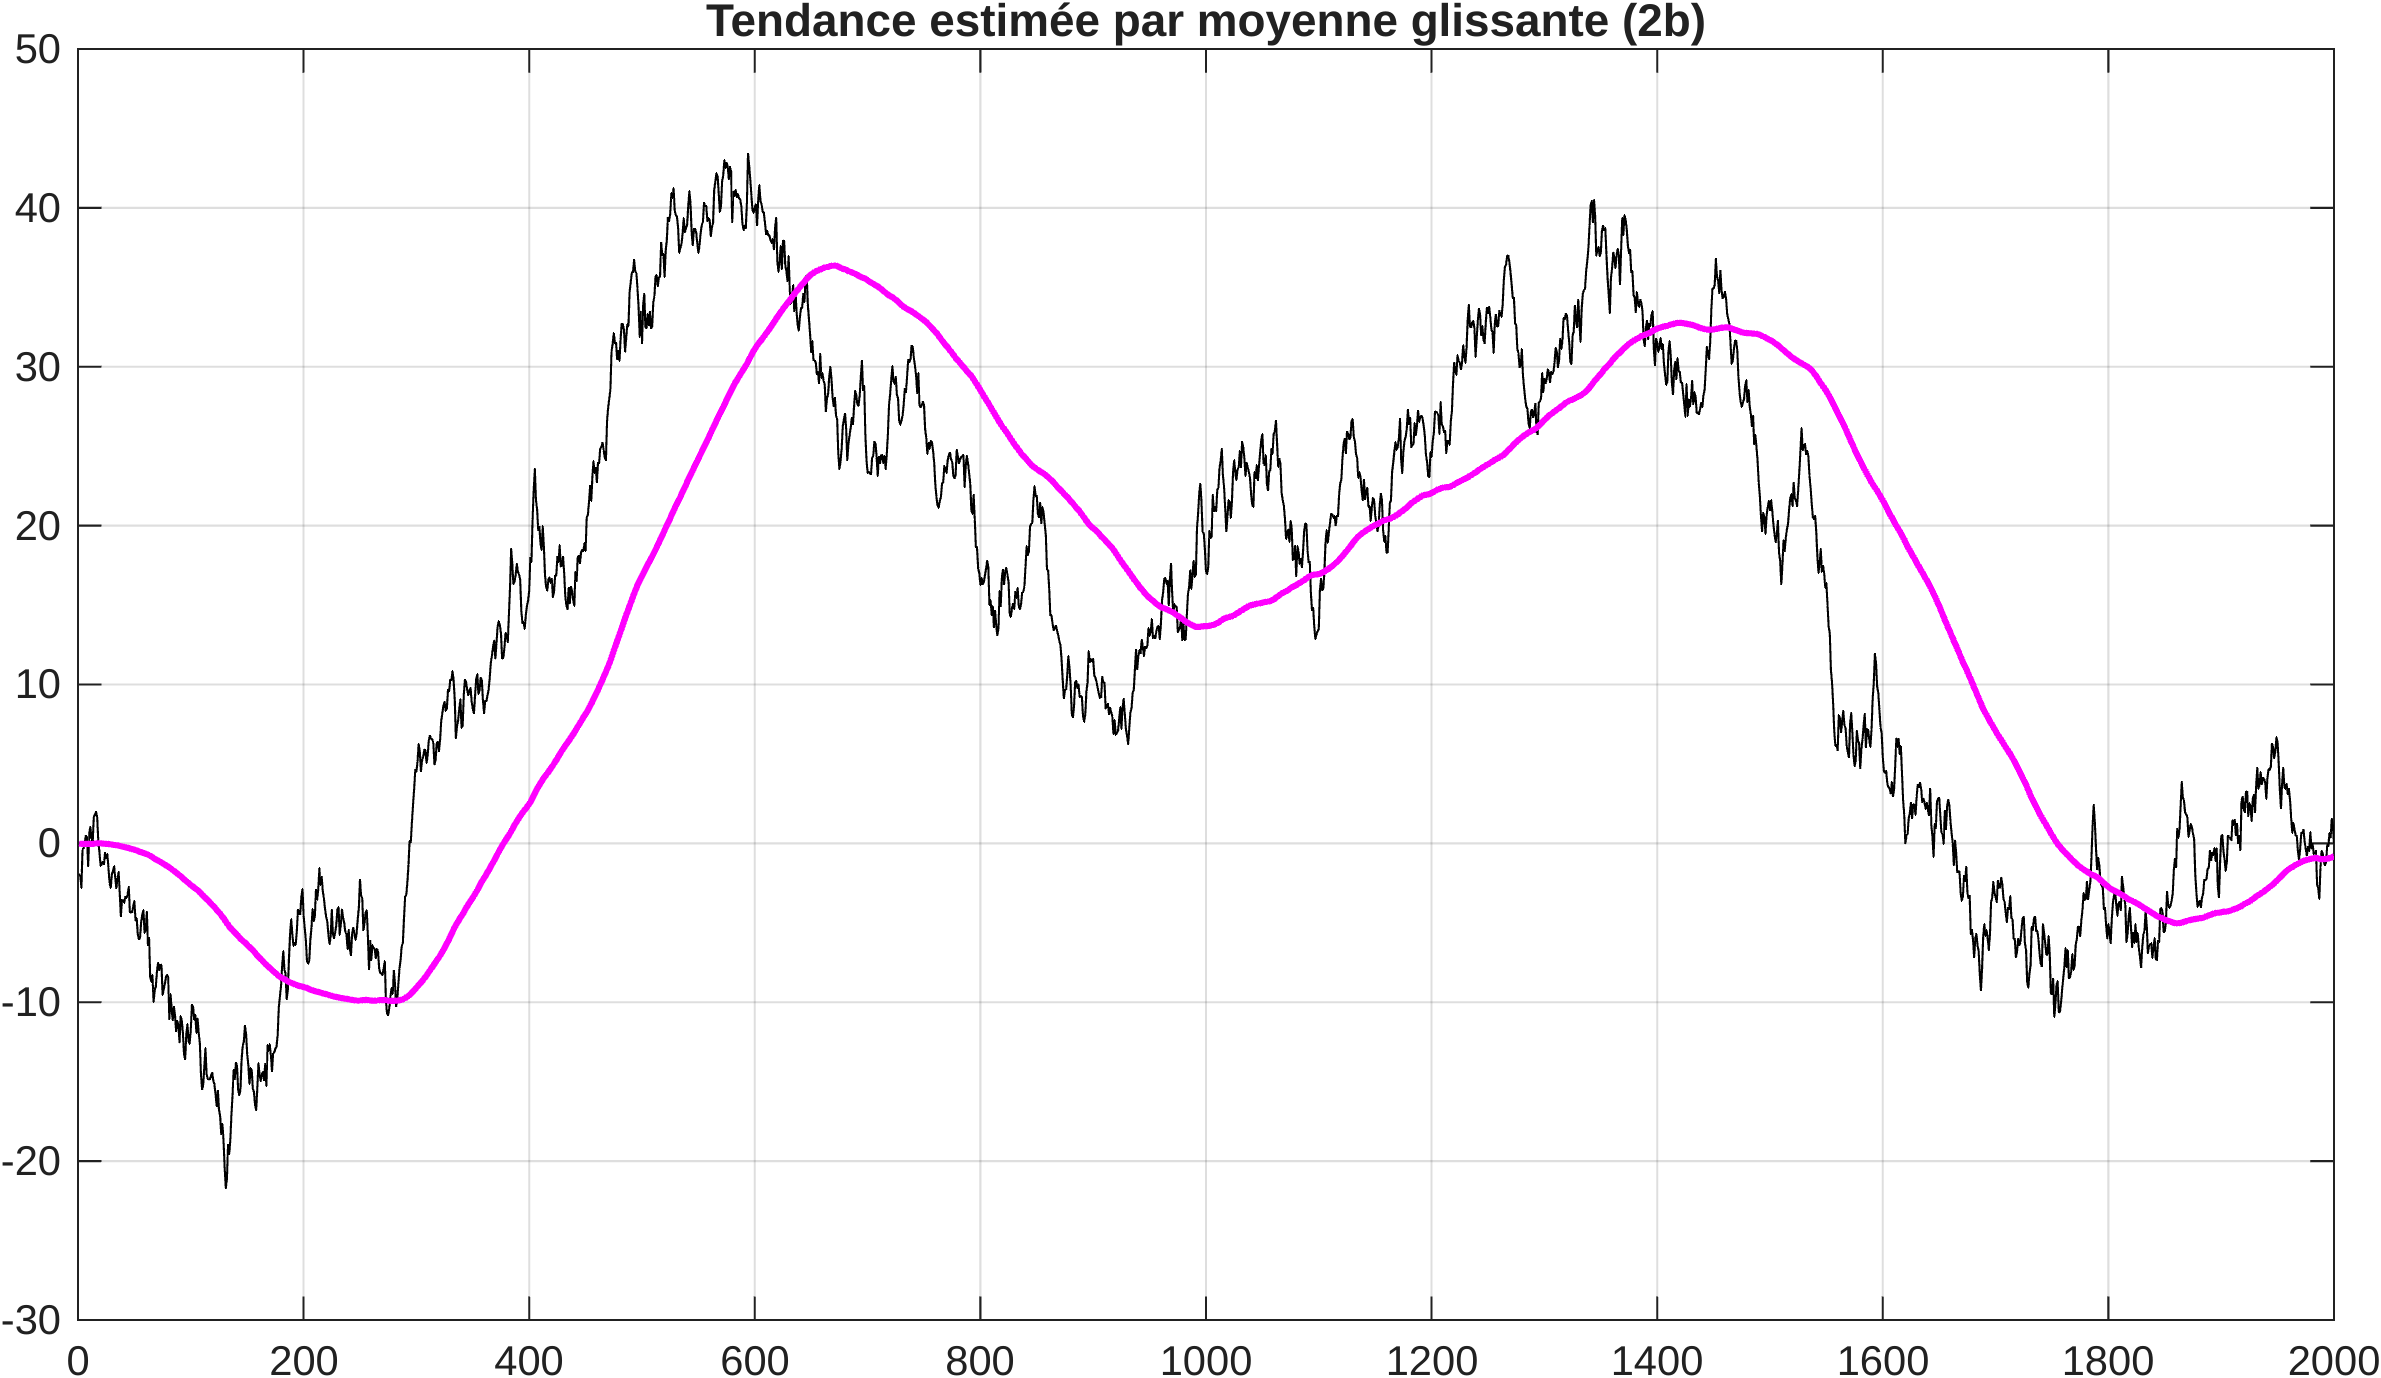
\includegraphics[width=0.7\linewidth]{fig16.png}
  \caption{Tendance estimée par moyenne glissante ($N = 200$).}
  \label{fig:mg}
\end{figure}

\paragraph{2c : filtrage à phase nulle}

Pour $h$ et $y$ réels, retourner le temps revient à conjuguer la transformée de Fourier :
$y(-n) \leftrightarrow Y^*(\nu)$.

\subparagraph{Stratégie 1.} On a $g(n) \leftrightarrow HY$, puis $r(n) \leftrightarrow H H^* Y^*$,
donc la sortie vérifie :
\begin{equation}
  r(-n) \;\longleftrightarrow\; |H(\nu)|^2\, Y(\nu).
\end{equation}
Le filtre équivalent $|H(\nu)|^2$ est réel et positif : la stratégie 1 est à phase nulle
pour tout filtre $h$ réel.

\subparagraph{Stratégie 2.} On a $g(n) \leftrightarrow HY$ et $r(-n) \leftrightarrow H^*Y$. En
divisant la somme par 2 pour garder un gain unité :
\begin{equation}
  \tfrac{1}{2}\big(g(n) + r(-n)\big) \;\longleftrightarrow\; \mathrm{Re}\{H(\nu)\}\, Y(\nu).
\end{equation}
Le filtre équivalent est réel, mais pas forcément positif : il n'est à phase nulle que si
$\mathrm{Re}\{H(\nu)\} \geq 0$. Ce n'est pas le cas de la moyenne glissante, dont la partie
reelle change de signe avant $1/N$.

\subparagraph{Choix de $h$.} La tendance correspond aux basses fréquences : $h$ doit être un
passe-bas. On a choisi la moyenne glissante de 2b, et on l'a comparée à des filtres
passe-haut, passe-bande et coupe-bande (figure~\ref{fig:strategies}). Seul le passe-bas
donne une vraie tendance, lisse et sans retard. Le passe-haut et le passe-bande oscillent
autour de 0, et le coupe-bande reste bruité. Avec la stratégie 2, la tendance est plus
aplatie, ce qui est cohérent avec la remarque précédente.

\begin{figure}[htbp]
  \centering
  \begin{subfigure}{0.49\linewidth}
    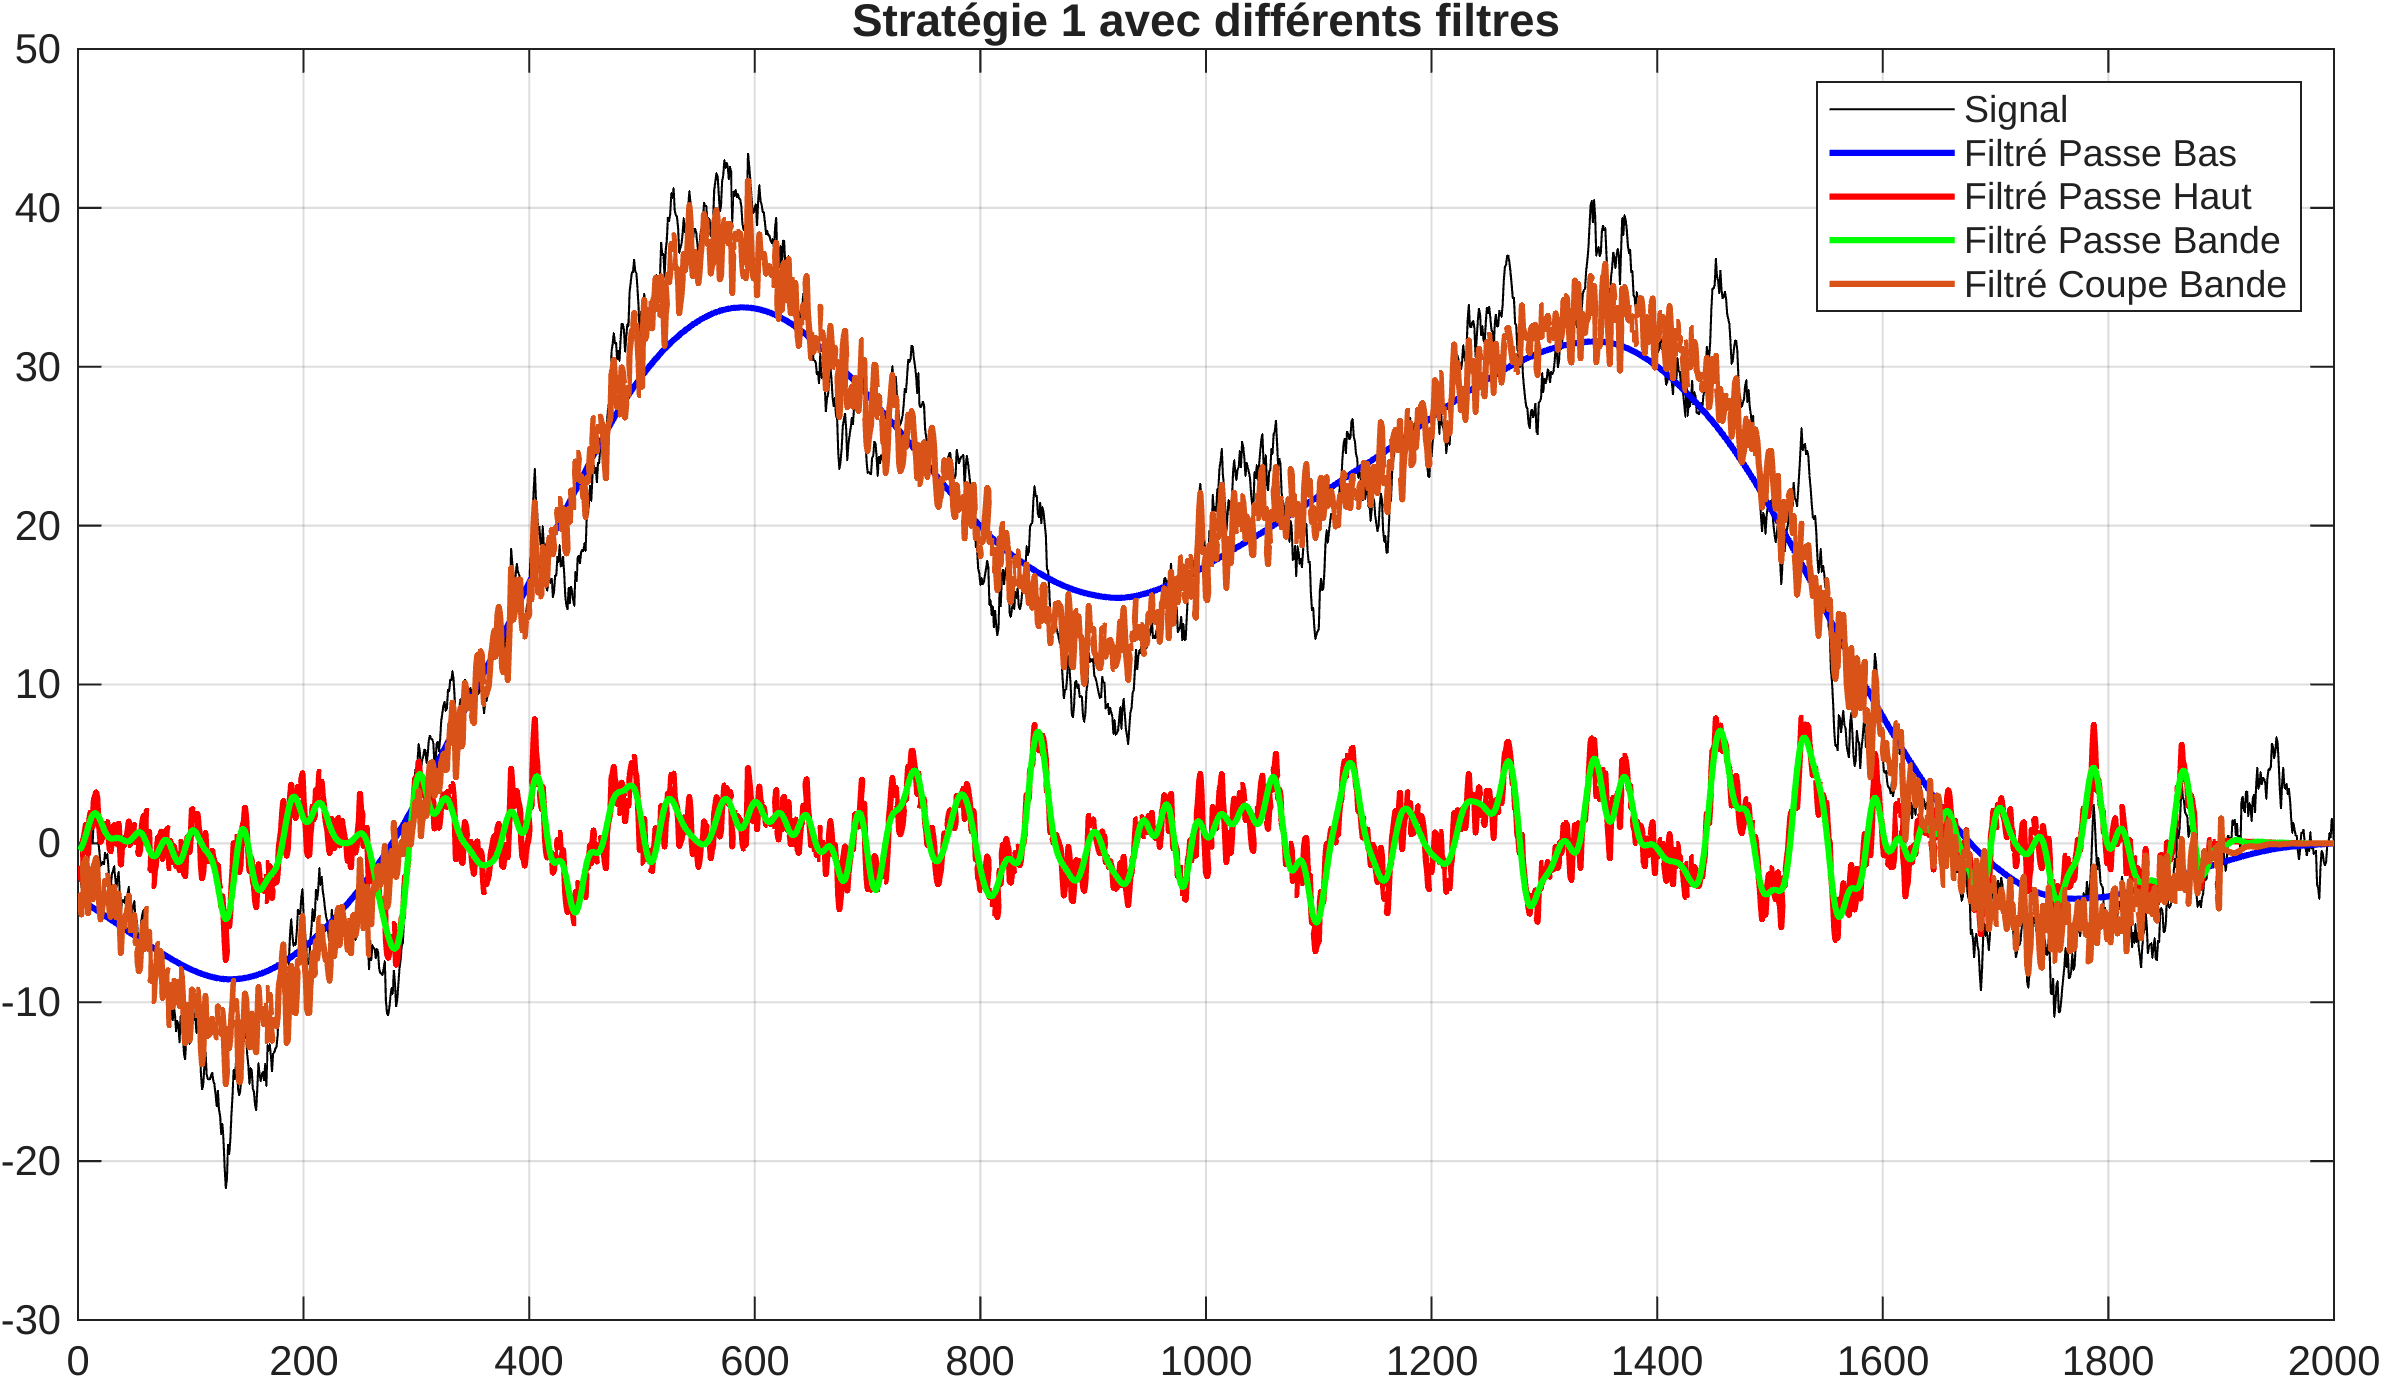
\includegraphics[width=\linewidth]{fig17.png}
    \caption{Stratégie 1}
  \end{subfigure}
  \begin{subfigure}{0.49\linewidth}
    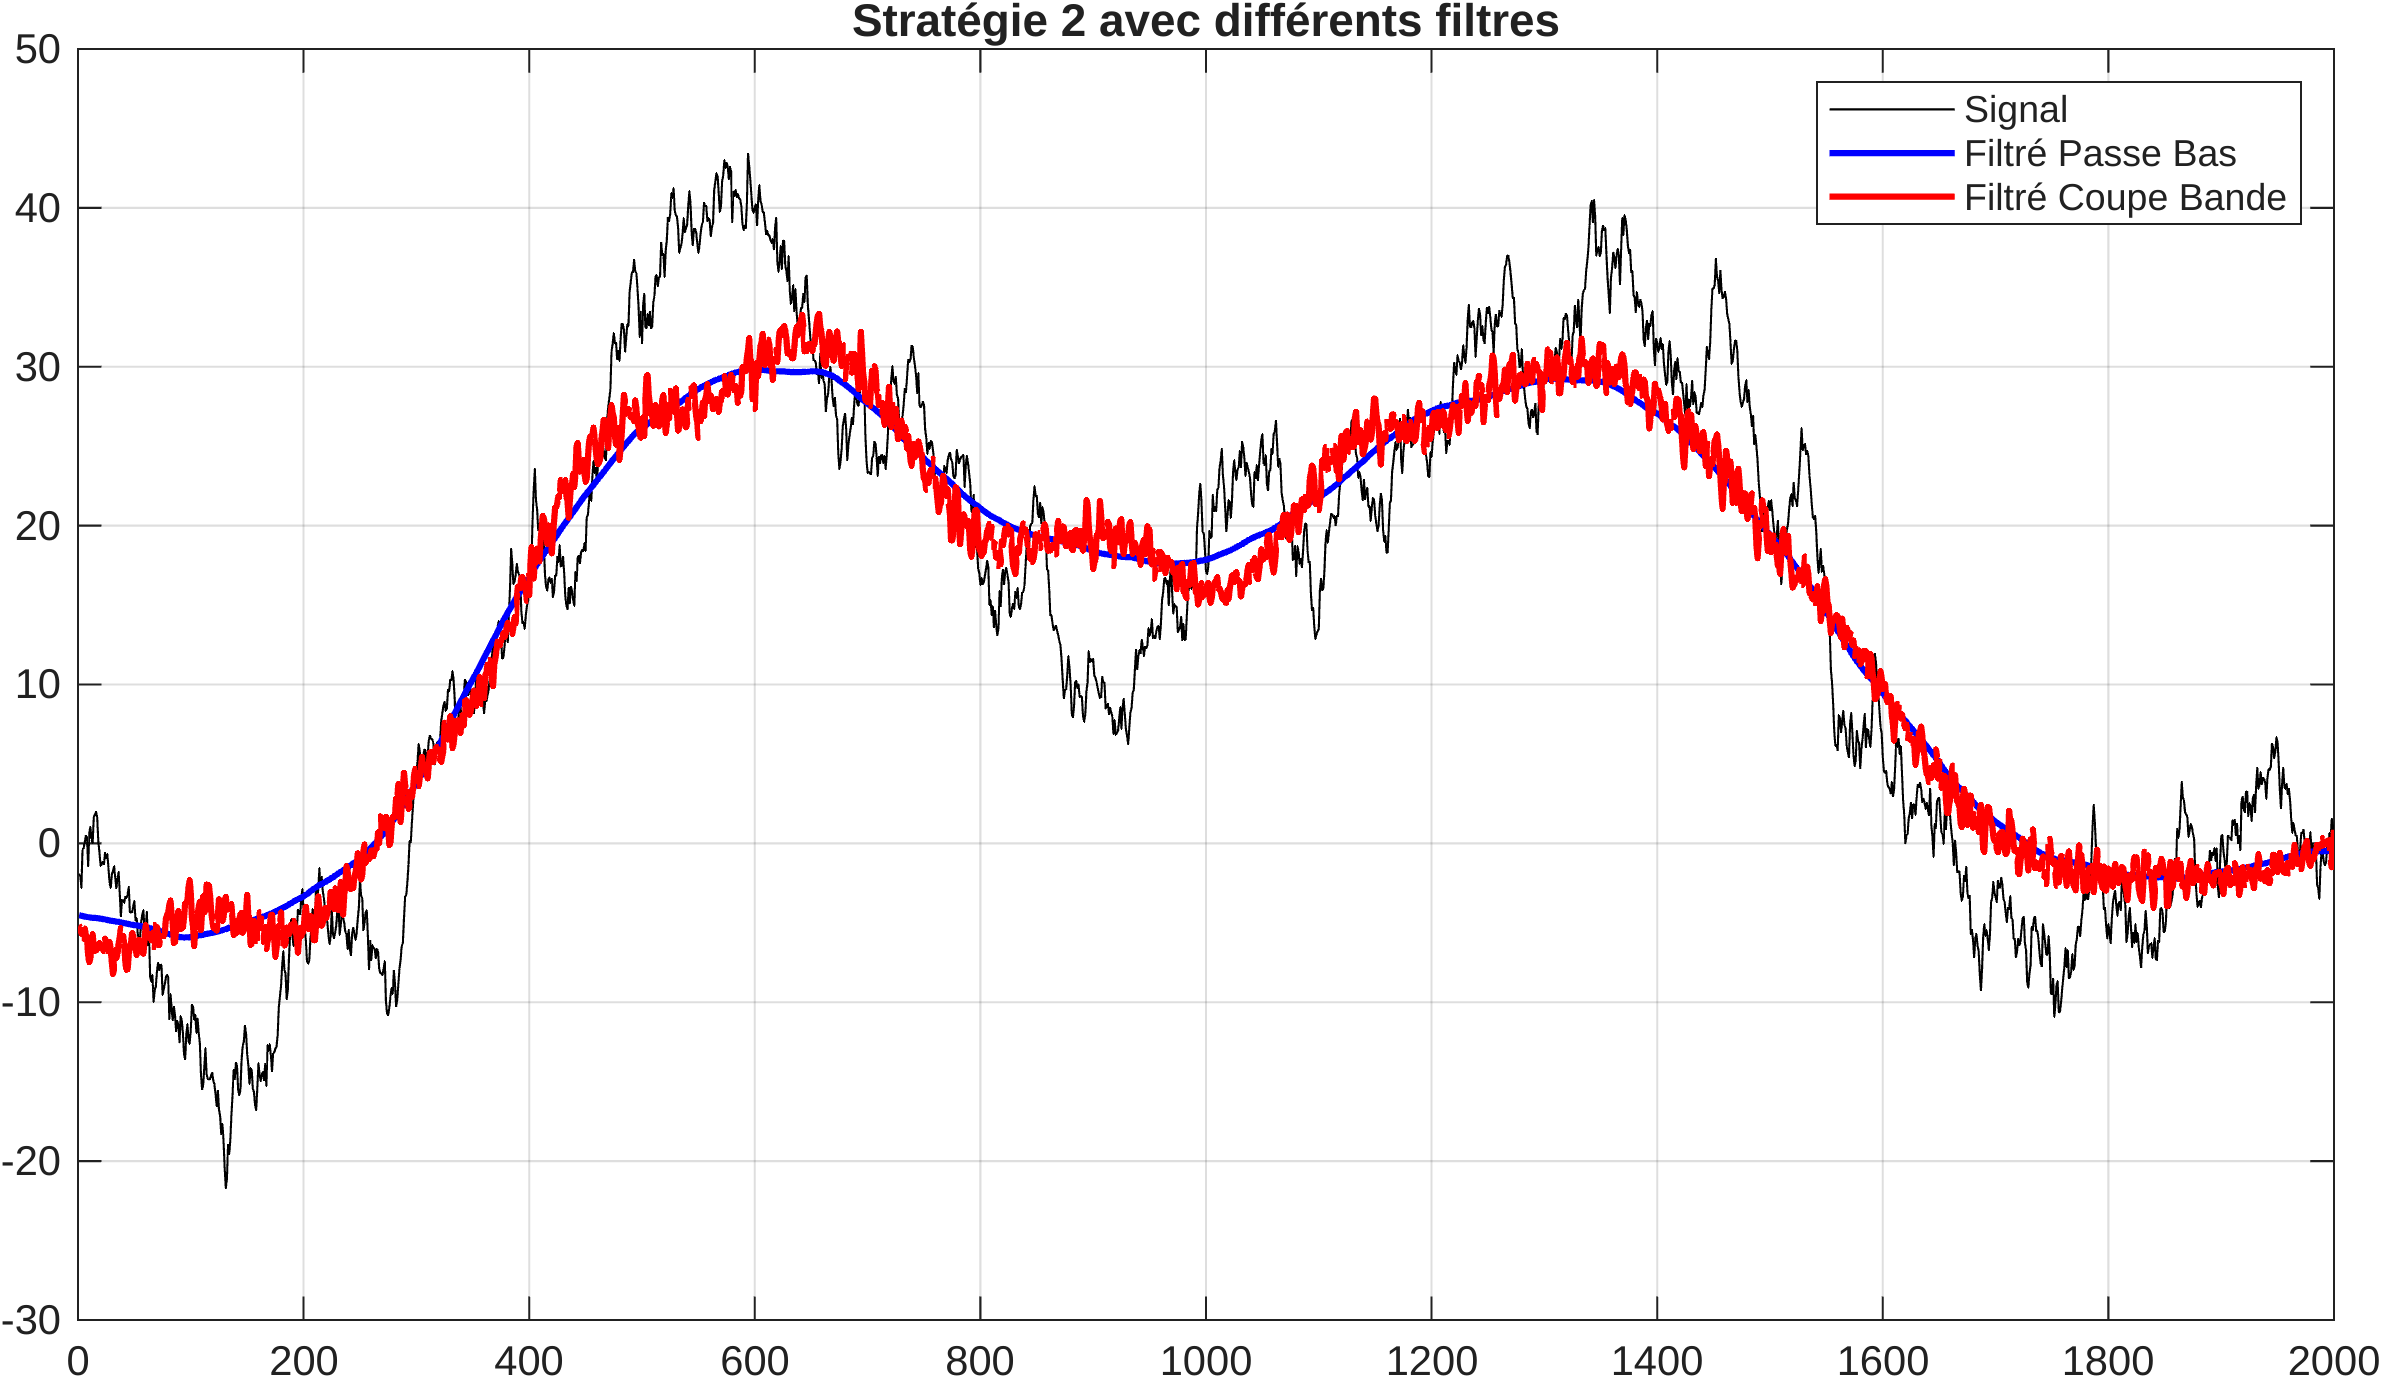
\includegraphics[width=\linewidth]{fig18.png}
    \caption{Stratégie 2}
  \end{subfigure}
  \caption{Filtrage à phase nulle de $y(n)$ avec différents filtres ($N = 200$).}
  \label{fig:strategies}
\end{figure}

\subsubsection{Étape n°3 : résidu et puissance}

Une fois la tendance estimée, on la retire au signal intégré pour obtenir le résidu :
\begin{equation}
  r(n) = y(n) - t(n).
\end{equation}
Ce résidu contient les fluctuations de $y(n)$ autour de sa tendance. Sa puissance moyenne
s'écrit, pour la méthode par blocs :
\begin{equation}
  P(N) = \frac{1}{LN} \sum_{n=1}^{LN} r^2(n)
       = \frac{1}{L} \sum_{l=1}^{L} \left( \frac{1}{N} \sum_{n=1}^{N} r_l^2(n) \right),
  \label{eq:PN}
\end{equation}
c'est-à-dire la moyenne des puissances du résidu calculées sur chaque bloc. Comme la matrice
$\mathbf{A}$ contient une colonne de 1, le résidu des moindres carrés est de moyenne nulle
sur chaque bloc : $P(N)$ correspond donc aussi à la variance moyenne du résidu.

Pour les méthodes par filtrage (2b et 2c), la somme porte sur les $M$ échantillons du
signal. Il vaut mieux cependant écarter les échantillons touchés par les régimes transitoires
des filtres, au début du signal et, pour les stratégies à phase nulle, aussi à la fin.

La puissance $P(N)$ dépend de la taille $N$ choisie. Pour $N$ petit, la tendance suit de
près le signal et le résidu est faible. Quand $N$ augmente, la tendance devient plus
grossière, et le résidu contient des fluctuations de plus en plus lentes, donc de plus en
plus grandes : $P(N)$ augmente avec $N$. C'est cette évolution que l'on étudie à
l'étape 4.

\subsubsection{Étape n°4 : représentation log-log et marqueur}

On calcule $P(N)$ pour toutes les valeurs de $N$ entre 3 et $M/2$, puis on trace
$\ln P(N)$ en fonction de $\ln N$. Pour les polynômes de degré $d \geq 2$, on commence à
$N = d+2$, sinon le polynôme passe par tous les points du bloc et $P(N) = 0$.

Les points obtenus sont ensuite approchés par une droite, toujours au sens des moindres
carrés : c'est le même calcul que \eqref{eq:mc} avec $d = 1$, appliqué aux couples
$(\ln N, \ln P(N))$. La pente $a$ de cette droite est le marqueur recherché.

Cette représentation a un intérêt : si $P(N)$ évolue comme une puissance de $N$,
$P(N) \propto N^{2\alpha}$, alors $\ln P(N) = 2\alpha \ln N + \text{cste}$, et les points
sont alignés sur une droite de pente $a = 2\alpha$. Pour un bruit blanc intégré, $y(n)$ est
une marche aléatoire, dont la variance croît linéairement avec le temps : on s'attend à
$P(N) \propto N$, donc à une pente $a = 1$.

\begin{figure}[H]
  \centering
  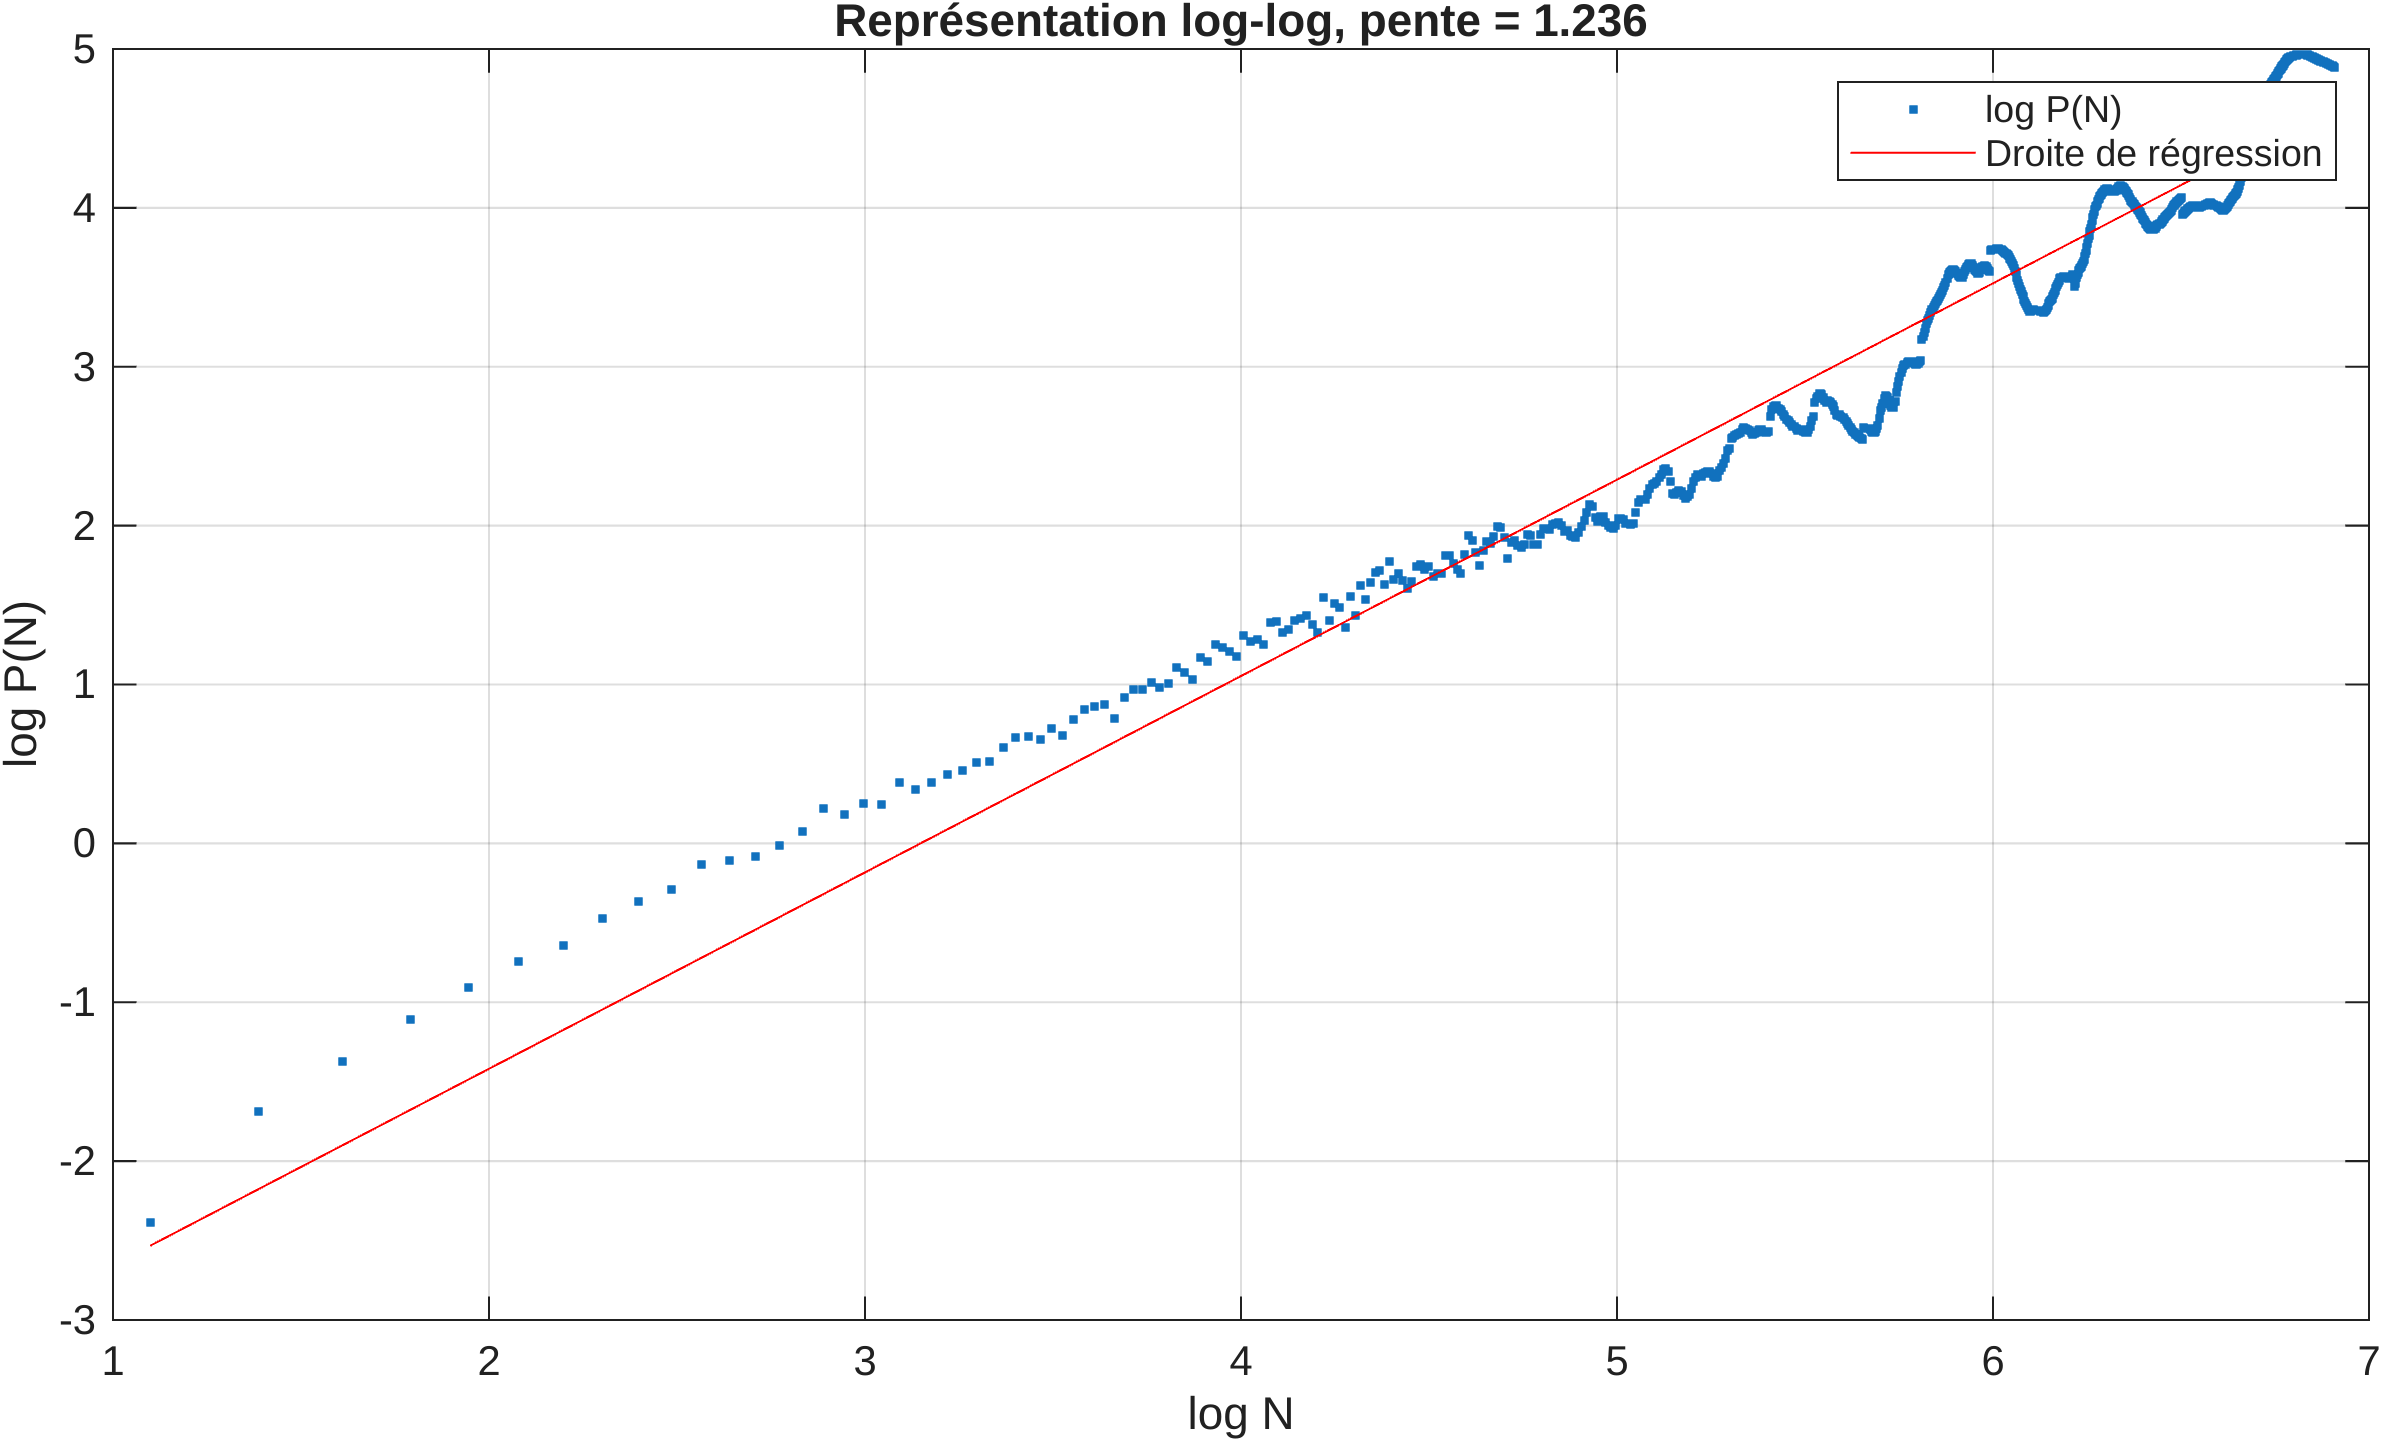
\includegraphics[width=0.65\linewidth]{fig19.png}
  \caption{Représentation log-log de $P(N)$ pour un bruit blanc intégré (tendance par
  droite, $M = 2000$) et droite de régression.}
  \label{fig:loglog}
\end{figure}

Sur la figure~\ref{fig:loglog}, la pente obtenue vaut $1{,}24$, un peu plus que la valeur
attendue. En regardant le nuage de points, on distingue trois zones :
\begin{itemize}
  \item pour les tout petits $N$, les points montent plus vite : avec seulement 3 ou 4
  échantillons par bloc, la droite ajustée colle presque au signal, et $P(N)$ est
  sous-estimé ;
  \item pour $N$ entre 10 et 150 environ, les points sont bien alignés, avec une pente
  proche de 1 ;
  \item pour les grands $N$, les points oscillent beaucoup. En effet, $P(N)$ n'est alors
  calculé que sur quelques blocs : dès que $N > 500$, il n'y a plus que 2 ou 3 blocs dans
  le signal.
\end{itemize}
Comme les valeurs de $N$ sont prises de 1 en 1, la moitié des points de la régression
correspond à $N > 500$, c'est-à-dire à la petite zone à droite du graphique, où
l'estimation est la moins fiable. C'est elle qui tire la droite et fausse la pente. Prendre
des valeurs de $N$ espacées de manière logarithmique, ou s'arrêter à un $N$ plus petit que
$M/2$, rendrait le marqueur plus fiable.

\section{Applications}

\subsection{Signaux testés}

On applique la méthode à deux signaux de $M = 2000$ échantillons :
\begin{itemize}
  \item \textbf{cas n°1} : un bruit blanc gaussien centré, de variance 1 ;
  \item \textbf{cas n°2} : un processus AR(2), obtenu en filtrant un bruit blanc par
  $1/A(z)$ avec $A(z) = 1 - 1{,}5\,z^{-1} + 0{,}7\,z^{-2}$. Ses deux pôles ont un module de
  $\sqrt{0{,}7} \approx 0{,}84$ et sont placés en $\nu \approx \pm 0{,}07$ : ce processus
  présente donc une résonance à basse fréquence, et ses échantillons sont corrélés sur
  quelques échantillons seulement.
\end{itemize}
La tendance est estimée par blocs (méthode 2a), pour des degrés $d$ allant de 0 à 3. On
calcule aussi le marqueur sans l'intégration de l'étape 1. Pour chaque cas, c'est la même
réalisation qui est utilisée pour tous les degrés : les différences entre les lignes du
tableau~\ref{tab:pentes} viennent donc uniquement de la méthode d'estimation de la tendance.

\begin{table}[H]
  \centering
  \begin{tabular}{|c|c|c|c|c|}
    \hline
     & \multicolumn{2}{c|}{Avec intégration} & \multicolumn{2}{c|}{Sans intégration} \\
    \hline
    Degré $d$ & Bruit blanc & AR(2) & Bruit blanc & AR(2) \\
    \hline
    0 & 0,58 & 0,77 & 0,02 & 0,05 \\
    1 & 0,84 & 0,83 & 0,03 & 0,14 \\
    2 & 0,93 & 0,79 & 0,05 & 0,21 \\
    3 & 0,93 & 0,93 & 0,06 & 0,26 \\
    \hline
  \end{tabular}
  \caption{Marqueur obtenu selon le degré de la tendance, avec et sans intégration
  ($M = 2000$, $N$ de 3 à $M/2$).}
  \label{tab:pentes}
\end{table}

\subsection{Avec l'intégration}

Pour le bruit blanc, les pentes sont comprises entre 0,58 et 0,93, alors que l'on attend
1. Ces écarts restent du même ordre que les variations d'une réalisation à l'autre : pour
$d = 1$, on obtient ici 0,84, contre 1,24 pour la réalisation de la
figure~\ref{fig:loglog}. Le marqueur est donc assez dispersé, pour les raisons vues à
l'étape 4.

Pour l'AR(2), on obtient des pentes très proches de celles du bruit blanc. Cela s'explique
par la mémoire courte de ce processus : ses échantillons ne sont corrélés que sur quelques
échantillons. Dès que $N$ est grand devant cette durée, le signal intégré se comporte comme
une marche aléatoire, exactement comme pour un bruit blanc. La différence entre les deux
processus n'apparaît que pour les très petites valeurs de $N$, qui ne représentent que
quelques points sur près de 1000 dans la régression. Avec la méthode telle qu'elle est
définie, le marqueur ne permet donc pas de distinguer ces deux signaux.

\subsection{Sans l'intégration}

Si l'on enlève l'intégration, les pentes deviennent beaucoup plus faibles :
\begin{itemize}
  \item pour le bruit blanc, elles sont presque nulles (0,02 à 0,06). Les échantillons étant
  indépendants, retirer une tendance ne change presque rien : la puissance du résidu reste à
  peu près égale à la variance du bruit, quelle que soit la valeur de $N$. La pente augmente
  légèrement avec $d$, car un polynôme de degré élevé retire un peu plus de puissance sur
  les petits blocs ;
  \item pour l'AR(2), les pentes sont plus grandes et augmentent nettement avec $d$ (de 0,05
  à 0,26). Sur les petits blocs, le polynôme arrive à suivre les oscillations lentes du
  processus et en retire une partie de la puissance : $P(N)$ est donc plus petit pour les
  petits $N$, ce qui augmente la pente.
\end{itemize}
Sans intégration, le marqueur sépare donc mieux les deux signaux qu'avec intégration. En
revanche, il perd son interprétation simple : la pente de 1 attendue pour un bruit blanc
intégré n'a plus d'équivalent.

\subsection{Réponses aux questions}

\paragraph{Le marqueur dépend-il de la manière d'estimer la tendance ?} Oui. Avec
intégration, la pente du bruit blanc passe de 0,58 pour $d = 0$ à 0,93 pour $d = 3$, sur la
même réalisation. La moyenne ($d = 0$) est la moins adaptée, car elle ne retire pas la
pente du signal à l'intérieur de chaque bloc. Entre $d = 1$ et $d = 3$, les écarts sont plus
faibles, du même ordre que la dispersion entre réalisations. Sans intégration, la
dépendance au degré est encore plus nette pour l'AR(2). Pour comparer des signaux entre
eux, il faut donc toujours utiliser la même méthode d'estimation. Les méthodes par filtrage
(2b et 2c) n'ont pas été testées ici : leurs régimes transitoires obligeraient à retirer
beaucoup d'échantillons pour les grandes valeurs de $N$.

\paragraph{Le marqueur dépend-il du nombre d'échantillons et des valeurs de $N$ ?} Pour le
bruit blanc intégré et $d = 1$, on obtient :
\begin{center}
  \begin{tabular}{|c|c|c|c|c|}
    \hline
    $M$ & 500 & 1000 & 2000 & 5000 \\
    \hline
    Pente & 0,91 & 1,18 & 0,74 & 1,19 \\
    \hline
  \end{tabular}
\end{center}
Les valeurs varient autour de 1, mais ne s'en rapprochent pas quand $M$ augmente. On
aurait pu penser qu'avec plus d'échantillons, le marqueur serait plus précis. Ce n'est pas
le cas, parce que $N$ va toujours jusqu'à $M/2$ : il reste toujours des valeurs de $N$ pour
lesquelles $P(N)$ n'est calculé que sur 2 ou 3 blocs, et ce sont elles qui faussent la
pente, comme on l'a vu à l'étape 4. Le marqueur dépend donc beaucoup des valeurs de $N$
choisies. Il serait plus fiable de limiter $N$ (par exemple à $M/10$), d'espacer les
valeurs de $N$ de manière logarithmique, ou de faire la moyenne du marqueur sur plusieurs
réalisations.

\section{Conclusion}

Ce projet a permis de mettre en pratique les concepts fondamentaux d'estimation spectrale et de filtrage numérique abordés en cours.

L'étude des périodogrammes a mis en évidence le compromis systématique entre résolution fréquentielle et variance de l'estimateur :
\begin{itemize}
    \item Le périodogramme standard présente une variance trop élevée qui ne diminue pas avec la taille de la séquence temporelle.
    \item L'estimateur de Daniell offre un lissage efficace sur des spectres à variations lentes (processus MA), mais montre rapidement ses limites face à des pics étroits (processus AR), où la taille de fenêtre admissible est trop faible pour réduire significativement le bruit sans déformer la résonance.
    \item L'estimateur de Bartlett permet de diviser la variance grâce au moyennage sur plusieurs blocs, mais il engendre d'importantes fuites spectrales à cause de sa fenêtre rectangulaire.
    \item L'estimateur de Welch s'avère être le plus performant : l'utilisation d'une fenêtre de Hann supprime les remontées spectrales et le recouvrement à 50\,\% maximise le nombre de blocs moyennés, assurant une forte diminution de la variance.
    \item Le corrélogramme de Blackman-Tukey constitue une alternative très efficace, particulièrement bien adaptée au processus MA où l'autocorrélation s'annule rapidement.
\end{itemize}

Concernant la méthode d'extraction du marqueur, nous avons constaté que le choix de la méthode d'estimation de tendance est déterminant. Si la moyenne glissante classique présente l'inconvénient d'introduire un retard de phase, la régression par blocs et le filtrage à phase nulle permettent d'isoler la composante lente de manière cohérente. La droite de régression en coordonnées log-log permet alors d'obtenir une pente stable, confirmant la validité de cette approche pour extraire un marqueur fiable en vue d'une classification de signaux.


\section{Organisation des Séances}

\section{Annexes}

L'ensemble des codes Matlab est fourni dans l'archive
\texttt{Cirou\_Paitard\_TSIG2.zip}, jointe au rapport. Le script principal
\texttt{main.m} permet de reproduire l'ensemble des figures présentées. Chaque fonction
précise en commentaire d'en-tête ses entrées, ses sorties et son objet.
La figure des spectres d'amplitude des deux processus n'a pas été jugé essentielle mais est présente dans les figure de l'archive.
\end{document}
